\input{fixos/pacotes}
\input{fixos/comandos}
\input{fixos/novosComandos}

% Dados pessoais
\autor{Macártur de Sousa Carvalho}
\curso{Engenharia de Software}

% Dados do trabalho
\titulo{Estudo de Métodos para redução do tempo de compilação em C++}
\data{2015}
\palavraChaveUm{redução do tempo de compilação}
\palavraChaveDois{c++}
\palavraChaveDois{llvm}
\palavraChaveDois{g++}
\palavraChaveDois{assembly}

% Dados da orientacao
\orientador{Prof. Dr. Edson Alves da Costa Júnior}
\coorientador{}

% Dados para a ficha catalográfica
\cdu{02:141:005.6}

% Dados da aprovação do trabalho
\dataDaAprovacao{01 de junho de 2013}
\membroConvidadoUm{Prof. Dr. Paulo Roberto Miranda Meirelles}
\membroConvidadoDois{Prof. Dr. Sérgio Antônio Andrade de Freitas  }

% Dados pessoais
\autor{Macártur de Sousa Carvalho}
\curso{Engenharia de Software}

% Dados do trabalho
\titulo{Estudo de Métodos para redução do tempo de compilação em C++}
\data{2015}
\palavraChaveUm{redução do tempo de compilação}
\palavraChaveDois{c++}
\palavraChaveDois{llvm}
\palavraChaveDois{g++}
\palavraChaveDois{assembly}

% Dados da orientacao
\orientador{Prof. Dr. Edson Alves da Costa Júnior}
\coorientador{}

% Dados para a ficha catalográfica
\cdu{02:141:005.6}

% Dados da aprovação do trabalho
\dataDaAprovacao{01 de junho de 2013}
\membroConvidadoUm{Prof. Dr. Paulo Roberto Miranda Meirelles}
\membroConvidadoDois{Prof. Dr. Sérgio Antônio Andrade de Freitas  }

\input{fixos/setup}

\usepackage{booktabs}
\usepackage{tabularx}
\usepackage[table,xcdraw]{xcolor}

% Setup
\lstset{numbers=left,
stepnumber=1,
firstnumber=1,
numberstyle=\tiny,
extendedchars=true,
breaklines=true,
frame=tb,
tabsize=2,
basicstyle=\footnotesize\ttfamily,
stringstyle=\ttfamily,
showstringspaces=false
}

\begin{document}

\frenchspacing 
\imprimircapa
\imprimirfolhaderosto*

\input{fixos/fichaCatalografica}
\input{editaveis/errata}
\input{fixos/folhaDeAprovacao}
%\input{editaveis/dedicatoria}
%\input{editaveis/agradecimentos}
\input{editaveis/epigrafe}
\begin{resumo}
Neste trabalho serão analisados métodos e ferramentas
 que proporcionem redução do tempo de compilação
 de programas escritos em C++, a fim de obter respostas mais
 rápidas às modificações no código e reduzir os gastos com recursos
 (humanos, de hardware e de tempo) utilizados no processo
 de compilação. Assim este trabalho consiste em uma
 análise preliminar de métodos e ferramentas que possam
 ser utilizadas em conjunto com o compilador g++ 
 nesta redução do tempo de compilação. Os métodos utilizados
 neste trabalho preliminar foram as guardas de inclusão,
 a declaração implícita de estruturas (\textit{forward declaration}),
 e processamento paralelo através do comando make.
 Os métodos analisados resultaram em uma redução média 
 do tempo de compilação em torno de 20\% e 40\%.

 \vspace{\onelineskip}
    
 \noindent
 \textbf{Palavras-chaves}: gcc. g++. c++. c. hpp. h.hxx. compilador. montador. gerador de código intermediário. forward declaration. declaração implícita.  guardas de inclusão externa. guardas de inclusão externa. redundância de guardas de inclusão. include. preprocessador. projeto. programa. pragma once. desenvolvedor. minutos. segundos. horas. semanas. compilação. código intermediário. desenvolvimento. equipes. empresas. fases da compilação. just in time. máquina virtual. ferramentas. metodologia. cronograma.

\end{resumo}

\begin{resumo}[Abstract]
 \begin{otherlanguage*}{english}

   This work will be analyzed methods and tools
 that provide reduced time of compiling C ++ programs,
 in order to obtain faster responses to changes in the code,
 deallocate resources (human, hardware and time) used in the
 build process. Thus, this work consists of a preliminary
 analysis of methods and tools that can be used along with
 the g ++ compiler in order to provide a reduction in compile
 time. Some methods used in this preliminary study were:
 inclusion guards, implicit declaration of structures
 (Forward Declaration), and parallel processing with makefile.
  These analysis methods have produced an average reduction of
 compilation time between 20 \% and 40 \%,.
   \vspace{\onelineskip}
 
   \noindent 
   \textbf{Key-words}: assembler. assembly. gcc. g++. c++. c. hpp. h.hxx. compiler. intermadiate code generator. forward declaration. external inclusion guards. internal inclusion guards. redundante inclusion guards. include. pre-processor. project. design. program. software. pragma once. developer. minutes. seconds. hours. weeks. compilation. development. team. busniss. compilation phases. just in time. virtual machine. tools. methodology. shedule.
 \end{otherlanguage*}
\end{resumo}

\input{fixos/listasAutomaticas}
\begin{siglas}
  \item[MV]   Máquina Virtual 
  \item[STL]  Standard Template Library 
\end{siglas}

\input{fixos/indiceAutomatico}

\textual

\part{Introdução}

\chapter*[Introdução]{Introdução}

Na computação, os primeiros computadores eletrônicos foram \lq\lq engenhocas monstruosas\rq\rq,
 que consumiam tanta energia quanto
 uma fábrica, e custavam, em 1940, milhares de dólares, com o poder
 computacional de uma calculadora moderna. Para os
 programadores que usavam estas máquinas a hora do computador era
 mais valiosas que a dele. E eles programavam em linguagem de
 máquina \cite[pág.5]{ref6}.

Programadores ou desenvolvedores são pessoas capazes de criar instruções
 que podem ser executadas por um computador, escrevendo o código-fonte em
 alguma linguagem de programação. Finalizado o código-fonte, a construção
 de um programa que será executado em um computador pode ser feita por um
 compilador, programa capaz de fazer a transformação de
 código-fonte escrito na linguagem de programação escolhida para uma linguagem
 entendível pelo computador, que é o código de máquina \cite[pág.5]{ref6}, a qual
 se trata de uma sequência de instruções binárias.
 Esta transformação recebe o nome de compilação \cite[pág.1]{ref5}.

Projetos de médio e grande porte gastam recursos e tempo a cada compilação,
 com perdas que dependem do hardware utilizado e do tamanho
 do projeto, sendo que a duração de um ciclo de compilação pode variar de
 alguns minutos até semanas \cite[pág.5]{ref6}. Neste contexto, este trabalho
 realizar um levantamento de métodos e ferramentas para redução do
 tempo de compilação, uma vez que esta redução pode significar ganhos
 significativos de recursos humanos, financeiros e no cronograma de
 desenvolvimento de equipes e empresas. 

\section*{Objetivos do Trabalho}

\subsection*{Objetivo Geral}

Analisar um conjunto de boas práticas e métodos para a redução do
 tempo de compilação de projetos escritos em C++ em diferentes ambientes,
 avaliando o impacto de cada estratégia.
 Serão selecionadas as melhores abordagens
 para os diferentes ambientes de desenvolvimento, tendo como meta conseguir uma
 redução mínima de 30\% no tempo de compilação dos projetos analisados. 

\subsection*{Objetivos Específicos}

Para conseguir atingir o objetivo geral do trabalho foram listados
 alguns objetivos específicos:

\begin{enumerate}
	\item Levantamento de métodos que envolvem a alteração de código fonte;
	\item Levantamento de métodos que envolvem a parametrização de build;
    \item Levantamento de ferramentas que podem auxiliar na compilação
 de projetos escritos em linguagem C++;
    \item Elencar projetos de código livre para análise do tempo de
 compilação;
    \item Coletar dados utilizando exemplos de uso de cada método aqui trabalhado,
 e avaliar o impacto de cada estratégia (método, ferramenta ou ambos)
 no tempo de compilação de cada projeto.
    \item Elencar as melhores abordagems para cada método analisado.
\end{enumerate}


\subsection*{Delimitação do Escopo}

Para delimitar o escopo e abrangência deste trabalho, e tornar possível
 a análise de projetos reais, será utilizado como referência uma linguagem
 de programação compilada conhecida por ser utilizada em sistemas embarcados,
 sistemas operacionais, sistemas críticos e jogos, dentre outras aplicações,
 que é a C++, criada por Bjarne Stroustroup \cite{BjarneC++}.

\subsection*{Organização do Trabalho}

O Capítulo 1 tem por objetivo introduzir o leitor nos conceitos abordados
 neste trabalho, descrevendo a diferença entre uma linguagem compilada e
 interpretada, o modelo \textit{just-in-time}, máquinas virtuais, o processo de compilação
 e suas etapas e os métodos a serem trabalhados.

O Capítulo 2 descreve um fluxo de trabalho realizado para a primeira etapa
 deste trabalho, contendo projetos escolhidos, ferramentas utilizadas e
 condução dos método aplicado.

O Capítulo 3 apresenta os resultados alcançados depois da aplicação dos métodos, coleta de dados,
 bem como uma analise e seleção dos métodos que obtiveram melhores resultados em cada ambiente.
 
Por fim o Capítulo 4 aprensenta as considerações finais e quais os trabalhos futuros
 poderiam ser realizados e que não foram abordados neste trabalho.

\part{Fundamentação Teórica}

\chapter[Fundamentação Teórica]{Fundamentação Teórica}

\section{Linguagens compiladas vs interpretadas}

Uma linguagem de programação é um método padronizado que possui
 um conjunto de instruções para realizar a comunicação entre o homem
 e o computador \cite{ref1} , através de um conjunto de regras
 definidas sintaticamente e sematicamente \cite{ref2}.
 Com uma linguagem
 de programação é possível especificar precisamente um conjunto de regras
 sobre  as quais dados serão armazenados ou transmitidos e criar algoritmos
 que facilitem operações ou resolvam problemas.
    
Para que um algoritmo escrito em uma linguagem de programação seja executado 
por um computador é necessário a criação de um arquivo de texto contendo um 
conjunto de palavras ou símbolos escritas de forma ordenada  e de maneira 
lógica \cite{ref3}. Este arquivo é chamado de código fonte.
    
Antes da execução, a linguagem de programação escrita no código fonte deve
 ser convertida (através do processo de compilação), traduzida (através do 
processo de interpretação) ou convertida e traduzida (forma hibrida) em um 
código de máquina \cite{ref4}.

\subsection{Compilação}

No processo de compilação a linguagem de programação contida no código fonte
 deve ser transformada em uma linguagem de máquina, a qual será posteriormente
 executada pelo processador \cite{ref2}. 

O processo de compilação requer a utilização de um compilador, o qual consiste
 em um programa ou conjunto de programas  que tem como entrada o código fonte 
escrito em uma linguagem de programação e cria um programa sematicamente 
equivalente uma outra linguagem, chamado de código objeto \cite{ref4}.

Após a compilação, a execução do código objeto criado a partir do algoritmo do
 código fonte de entrada é requisitado pelo usuário para que o processador 
execute as instruções de máquina \cite{ref6}.

As linguagens que, em geral, são compiladas, lideram em performance em relação
 as linguagens que, em geral, são interpretadas. Isso porque as decisões que são
 tomadas em tempo de compilação não são necessários no tempo de execução \cite{ref7}.
Por exemplo, se um compilador garantir que uma variável x seja sempre alocada 
em uma  mesma posição na memória,  ele pode gerar instruções de maquina que 
acesse esta localização sempre que se referenciar a variável x. 
Por outro lado, um interpretador precisa procurar  por x em uma tabela a cada 
acesso, a fim de achar sua localização \cite{ref8}.

\begin{description}
    \item[Exemplos de Linguagem que, em geral,são compilada:]\
    \begin{itemize}
      \item  Ada
      \item  ALGOL
      \item  BASIC
      \item  C
      \item  C++
      \item  COBOL
      \item  Cobra
      \item  Common Lisp
      \item  D
      \item  Delphi
      \item  Eiffel
      \item  Fortran
      \item  Objective-C
      \item  Pascal
      \item  Visual Basic
      \item  Visual Prolog
    \end{itemize}
\end{description}

\subsection{Interpretação}

No processo de interpretação, o código fonte é passado para um programa chamado
 interpretador, o qual é responsável pela leitura do código e pela tradução, 
em tempo real, deste código em instruções a serem executadas pelo sistema 
operacional ou  pelo processador \cite{ref8}. No caso de linguagens que são, em geral, 
interpretadas, costuma-se nomear os códigos-fonte como scripts, embora não seja 
uma regra geral.

Ao contrário do compilador, o interpretador faz a leitura do código fonte e 
executa  as respectivas instruções em tempo real. Isso faz com que  códigos 
interpretados tenham maior flexibilidade e um melhor diagnóstico (exibição de 
mensagens de erros) do que  códigos compilados. A interpretação também pode lidar 
melhor com linguagens de programação nas quais características fundamentais, 
tais como  o tamanho e  o tipo das variáveis, podem depender dos dados de 
entrada \cite{ref6}.

Sem  o recurso da interpretação, seria uma tarefa deveras complexa implementar 
alguns recursos  presentes em linguagens Lisp e Prolog onde, por exemplo, 
um programa pode escrever novas peças de si mesmo e executá-las em tempo real
 \cite{ref6}.

\begin{description}
    \item[Exemplos de Linguagem que, em geral, são interpretadas:]\
    \begin{itemize}
        \item ActionScript
        \item APL
        \item ASP
        \item BASIC
        \item C\#
        \item CYBOL
        \item Java
        \item JavaScript
        \item Lisp
        \item Logo
        \item Lua
        \item PHP
        \item Python
        \item Ruby
        \item Scheme
        \item Smalltalk
        \item VBScript
    \end{itemize}
\end{description}

\subsection{VM}

Para algumas linguagens existe o caso em que o compilador tem o papel
 de converter o código fonte em um \textit{byte code}\cite{ref9}. 
O \textit{byte code}
é uma linguagem de baixo nível  similar a linguagem de máquina, que 
deve ser interpretada por um outro programa chamado Maquina Virtual. 

Esta estratégia mista de pré-compilar o código para uma linguagem 
intermediária e interpretá-la em uma máquina virtual é denominada 
estratégia hídriba. 

\begin{description}
    \item[Exemplos de linguagens que utilizam, em geral, 
          a estratégia híbrida, são:]\
    \begin{itemize}
        \item Java  
        \item Python
        \item JRuby
        \item Oxygene
        \item Rhino
        \item Nashorn
        \item JGNAT
        \item Jython
        \item Rakudo Perl 6
    \end{itemize}
\end{description}

\subsection{JIT}

O termo \textit{Just In Time} - JIT - veio de um novo modelo de  negócio da
 indústria manufatureira : uma estratégia de negócio onde a produção 
ou compra era feita sobre demanda, ao invés da utilização de estoques
 \cite{ref10}. 
Este modelo tem como vantagens menores custos com armazenamento, 
menos desperdícios, resposta mais rápida aos clientes e maior 
produção potencial.

Na compilação, esta analogia se adapta bem por que um compilador JIT 
não armazena os binários do programa no disco (o estoque), mas começa 
a compilação apenas de partes do programa necessárias durante a execução
 \cite{ref11}.

Foram desenvolvidas, principalmente para linguagens que são, em geral, 
interpretadas, ferramentas que se valem do JIT para acelerar a interpretação
 e execução dos códigos-fonte (scripts) como, 
por exemplo, o PyPy para a linguagem Python.\footnote{http://pypy.org/}


\section{Compilação}

\subsection{Pré-processadores}


Antes de um código-fonte passar pelo processo de compilação, pode ser
 necessária a execução de um programa, denominado pré-processador, que
 tem como responsabilidade preparar o código-fonte para a compilação. 

Dentre as possíveis tarefas e caracerísticas comuns a um pré-processador,
 podemos citar:

\begin{itemize}

\item \textit{Processamento de macros}: um pré-processador pode permitir que um usuário 
    defina macros que sejam abreviações para construções mais longas\cite{ref11};

\item \textit{Inclusão de arquivos}: um pré-processador pode incluir arquivos cabeçalho no
     texto do programa. Por exemplo, o pré-processador faz com que o conteúdo de
     um arquivo externo seja transcrito no código-fonte no ponto onde existe a 
    marcação para sua inclusão\cite{ref11};

\item \textit{Pré-processadores “racionais”}: este tipo de pré-processador é responsável 
    por permitir a construção de macros utilizando condicionais while ou if mesmo
     em linguagens que não suportem tais estruturas\cite{ref11};

\item \textit{Extensões de linguagens}: são formas de conferir maior poder as linguagens
     através de macros embutidas. Por exemplo, 
    Equel \footnote{Equel:  http://www.eecs.berkeley.edu/~wong/wong\_pubs/wong46.pdf
     acessado 11/junho p.6} é uma linguagem de 
    interrogação embutida em C que permite a manipulação de banco de dados. 
    Os enunciados começados com \#\# são considerados pelo pré-processador como
     comandos de acesso ao banco de dados, os quais não fazem parte da 
    linguagem C e, quando traduzidos, são convertidos em rotinas que tratam 
    este acesso ao banco de dados\cite{ref11}.

\end{itemize}

\subsection{Compilação}

No processo de compilação tradicional, o compilador atua em duas fases 
principais: análise e síntase\cite{ref12}\cite{ref13}. A Figura \ref{fig01}
 ilustra estas fases. 

\begin{figure}[h]
    \centering
        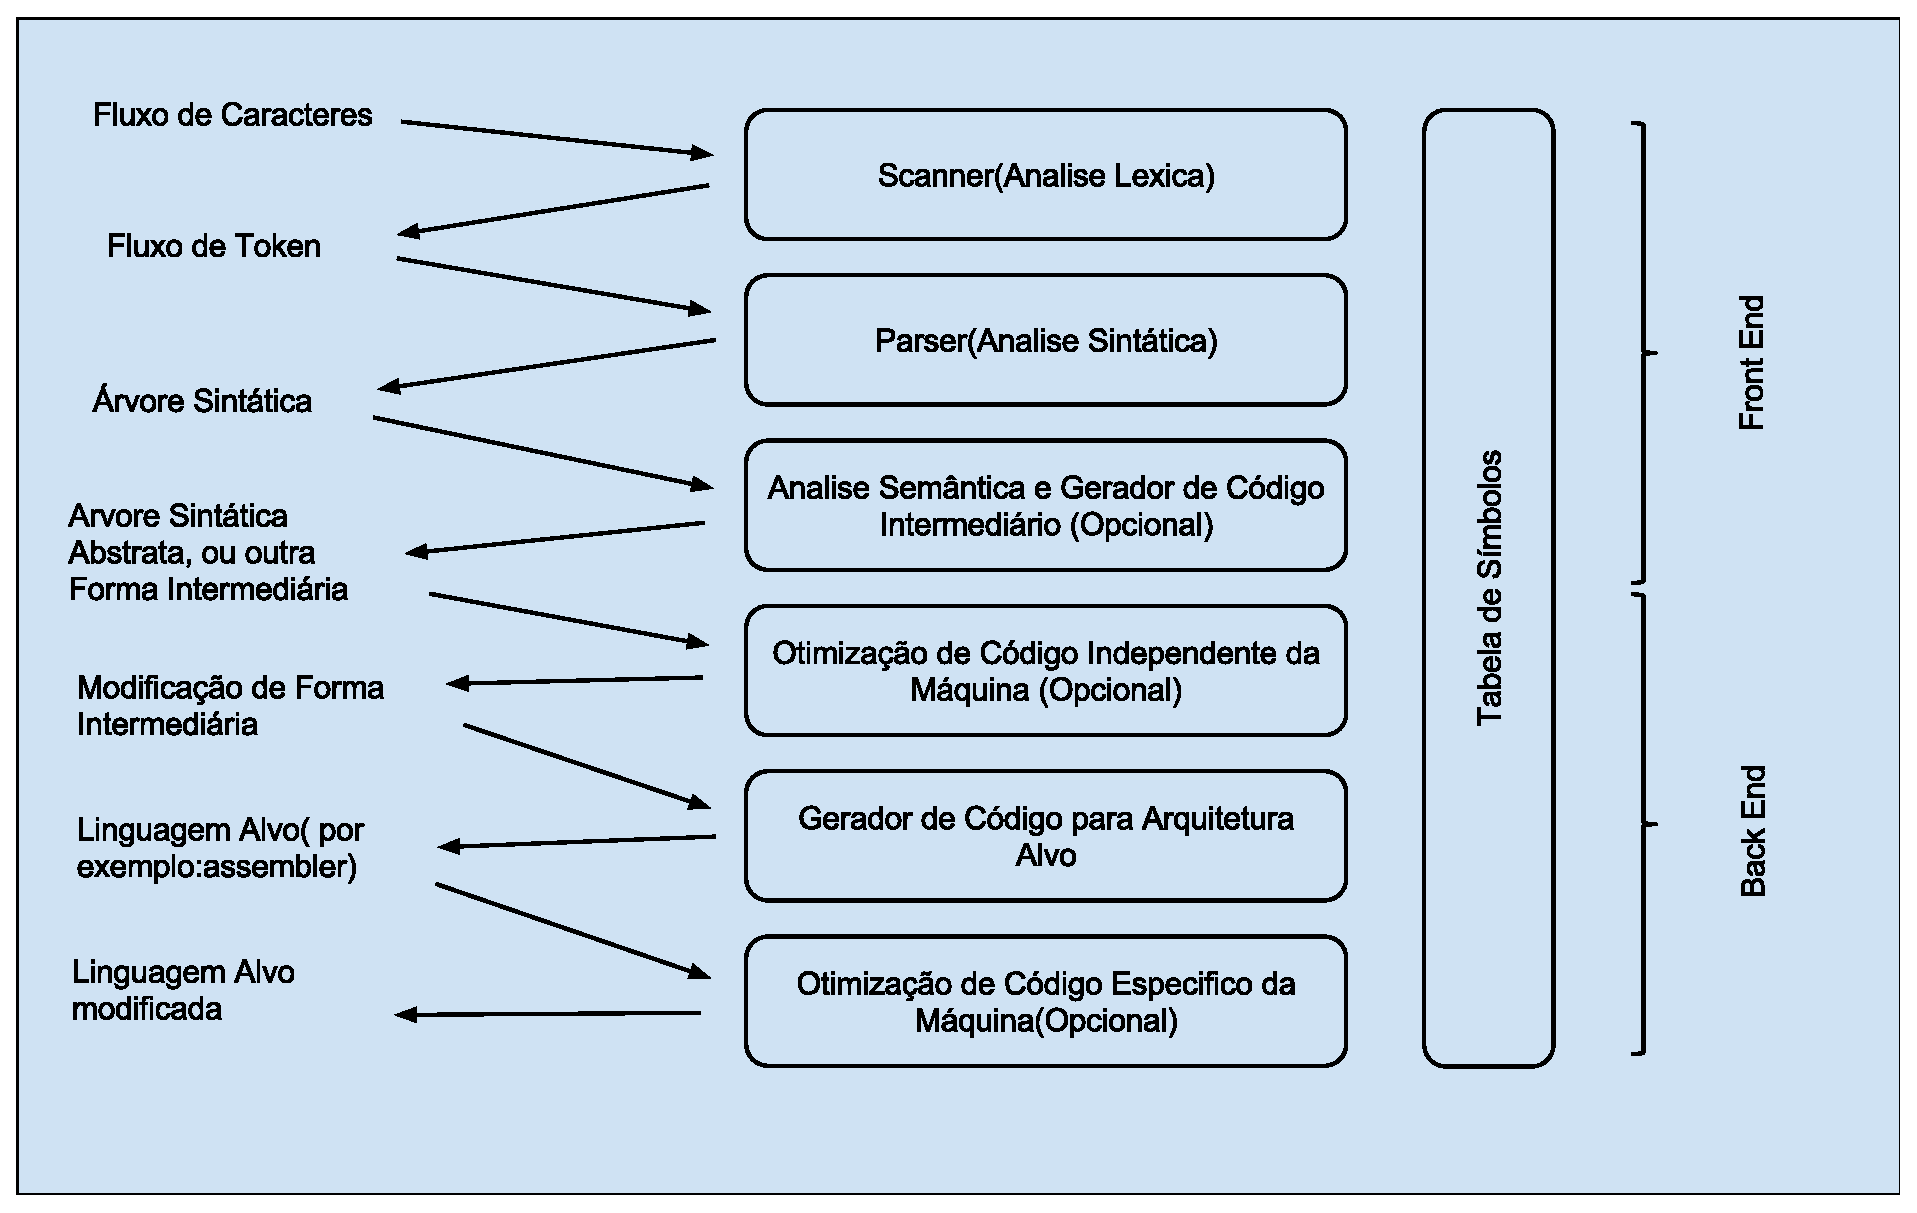
\includegraphics[keepaspectratio=true,scale=0.5]{figuras/fases_da_compilacao.eps}
    \caption{Fases da Compilação, (Scott, Michael L.,2008)  com adaptações.}
    \label{fig01}
\end{figure}

A fase de analise (ou \textit{front-end}) de um compilador é a fase que 
tem como objetivo entender o código fonte e  representá-lo em uma 
estrutura intermediária que facilite sua manipulação posterior. 
Esta fase é subdividida em analise léxica, analise sintática, 
analise semântica e geração de código intermediário \cite{ref14}.

A fase de síntese (ou \textit{back-end}) de um compilador é a fase que tem 
como objetivo realizar a geração de código final otimizando o código 
analisado na fase de sintase, gerando um código sematicamente igual ao 
código fonte e com melhorias de performance e espaço. Esta fase é 
subdividida em otimização de código independente do alvo, geração de 
código alvo, otimização de código  para o alvo específico \cite{ref14}.


\subsection{Analise Léxica}
    
A analise léxica é a primeira fase a ser executada pelo compilador \cite{ref15}. 
A função do analisador léxico, também denominado scanner, é ler o código fonte, 
caracter a caracter, buscando a separação e  a identificação dos elementos do 
programa, denominados símbolos léxicos ou tokens \cite{ref16}. Assim, é 
produzida uma sequência de tokens que será utilizada na análise sintática \cite{ref17}. 

Esta fase também tem a importância de realizar a remoção de elementos 
“decorativos” do programa, tais como espaços, tabulações, caracteres de 
avanço e comentários \cite{ref15}. Para auxiliar a construção deste analisador,
 estão disponíveis uma série de geradores automáticos de analisadores léxicos, 
cujo objetivo é reduzir o esforço de programação deste tipo de ferramenta, 
especificando-se apenas os tokens a serem reconhecidos \cite{ref18}.

\subsection{Analise Sintática}

A analise sintática, ou analise gramatical, é o processo de se determinar 
se uma cadeia de símbolos léxicos pode ser gerada por uma gramática pré-definida
 \cite{ref19}. O analisador sintático é o responsável por verificar se os 
símbolos contidos no código fonte formam um programa válido ou não \cite{ref20}.

A maioria dos métodos de analise sintática são de dois tipos, denominados 
\textit{top-down} ou \textit{bottom-up} \cite{ref21}. Como indicado por 
seus nomes, os analisadores sintáticos \textit{top-down} constroem árvores 
do topo para as folhas, enquanto o analisadores \textit{bottom-up} começam das 
folhas e constroem a árvore de baixo para cima até chegar na raiz. Em ambos os
 casos  estas árvores  elas são percorridas da esquerda para a direita, 
simbolo a simbolo. Estes dois tipos são utilizados devido seu potencial 
expressivo para descrever a maioria das construções sintáticas das linguagens 
de programação \cite{ref20}. Para auxiliar na criação de analisadores sintáticos 
existem disponíveis uma série de geradores automáticos, como por exemplo, 
o \textit{Flex} 
\footnote{Flex: encontrado em http://dinosaur.compilertools.net/ acessado dia 
20/06/2015}, 
o \textit{Bison} 
\footnote{Bison: econtrado em http://www.gnu.org/software/bison/ acessdo dia 
20/06/2015}
 e o \textit{JavaCC} 
\footnote{JavaCC: encontrado em https://javacc.java.net/ acessado dia 20/06/2015}
 \cite{ref22}.

\subsection{Analise Semântica}

O analisador semântico tem como função prover métodos para que as estruturas 
construídas pelo analisador sintático possam ser avaliadas ou executadas \cite{ref23}. 
Estas validações são feitas para assegurar que certos tipos de erros de 
programação sejam detectados e reportados. Os  exemplos de verificação incluem 
declaração de tipo, declaração de funções, sobrecarga de funções, sobrecarga de 
operadores, verificação de fluxo de controle, verificação de operações logicas e 
aritméticas válidas entre variáveis e a verificação de unicidade de variáveis em 
determinados escopos da linguagem \cite{ref24}.

\subsection{Gerador de Código Intermediário}

Após produzir uma árvore sintática sematicamente correta, o compilador é capaz de
 produzir uma linguagem de representação intermediária do código fonte. Uma linguagem 
intermediária está mais próxima de uma linguagem de objeto do que do código fonte. 
No entanto, a linguagem  intermediária permite uma manipulação mais fácil do que o 
código de maquina ou o \textit{Assembly} \cite{ref25}. 

Um tipo bem conhecido de linguagem intermediara é o código (ou sentença) de três 
endereços\cite{ref26}. Este código é uma sequência de enunciados na forma geral, apresentada 
 no Código \ref{codigo01}.


\begin{lstlisting}[language=C++,frame=single,captionpos=b,caption={
								Código de três endereços},
											label=codigo01]
   x:=y op z
\end{lstlisting}


onde \textbf{x}, \textbf{y}, \textbf{z} são nomes, constantes ou objetos de dados 
temporários criados pelo compilador e \textbf{op} representa um operador qualquer,
 tal como um operador de ponto fixo, flutuante ou um operador lógico sobre dados
 booleanos \cite{ref27}. Uma forma prática de representar sentenças de três endereços é o uso
 de quádrupla (operador, argumento 1, argumento 2 e resultado). 
Este esquema de representação de código intermediário é o preferido por diversos
 compiladores, principalmente por aqueles que executam extensivas otimizações de
 código, uma vez que o código intermediário pode ser manipulado mais 
facilmente \cite{ref28}. Além destas representações existem outras como as 
árvores, grafos acíclicos dirigidos (DAG) e a notação polonesa \cite{ref29}.

Para garantir que um código tenha o seu desempenho ampliado e utilize menos 
espaço em disco, a fase de otimização de código busca examinar 
estrategicamente o código intermediário produzido na fase anterior e, com o 
uso de técnicas de otimização, produzir um código mais eficiente \cite{ref30}
. A otimização de código pode ocorrer em duas etapas: uma após a geração de 
código intermediário e a outra depois da geração do código para a máquina 
alvo \cite{ref31}. 
Para a execução desta etapa são utilizadas técnicas para detectar 
padrões dentro de um código produzido e substituí-los por códigos mais
 eficientes \cite{ref28}. Entre as técnicas usadas realizadas estão a 
substituição de expressões que podem ser calculadas durante o tempo 
de compilação, movimentação de código, eliminação de sub-expressões 
redundantes, desmembramento de laços, eliminação de variáveis de indução, 
substituição de multiplicação pelo \textit{shift} binário, redução da 
quantidade de laços, entre outras \cite{ref30}.

\subsection{Geração de Código}

Gerador de código é a parte ou componente do compilador responsável por 
realizar a o mapeamento da linguagem intermediária otimizada para a linguagem 
alvo. Caso a linguagem alvo seja um código de máquina,  registradores ou 
localização de memoria são selecionados para armazenar valores das 
variáveis usadas no programa. Então, o código intermediário é traduzido em 
sequência para instruções de máquina que realizarão as operações \cite{ref32}.
Mesmo que o código traduzido seja otimizado, após a tradução para a 
linguagem alvo é  possível que novas otimizações possam ser feitas, de modo 
que é possível a otimização especifica apresentada nas Figura \ref{fig02}.

\begin{figure}[h]
    \centering
        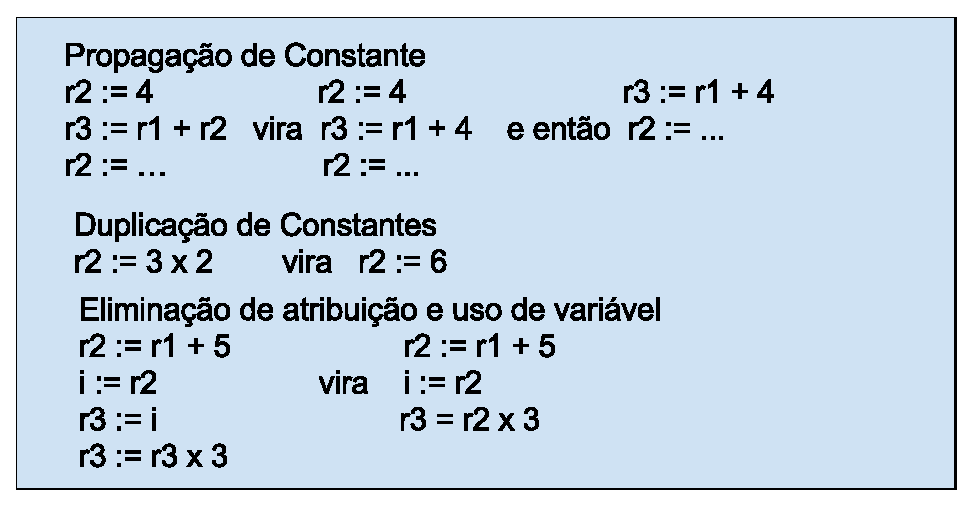
\includegraphics[keepaspectratio=true,scale=0.7]{figuras/otimizacao_especifica.eps}
    \caption{Exemplos de Otiminizações especificas,
             (Scott, Michael L.,2009) com adaptações }
    \label{fig02}
\end{figure}


\subsection{Assembly}

Segundo Michael L. Scott, um código de máquina é uma sequência de bits que
 corresponde a uma instrução executada por um processador, realizando 
operações de adições, comparações, movimento de informação de uma localização
 da memória, entre outros. Detalhar instruções de máquina a nível de bits é 
uma tarefa trabalhosa \cite{ref34}. 

Um programa capaz de realizar o cálculo do máximo divisor comum através do 
algoritmo de Euclides estendido pode ser representado  em código de máquina 
usando notação hexadecimal para a representação dos bits, conforme apresentado
 no Código \ref{codigo_02} \cite{ref34}.


\begin{lstlisting}[language=Pascal,frame=single,captionpos=b,
												caption={Algoritmo de 
									   Euclides estendido representado 
									   em código de máquina,com adaptações},
                                                            label=codigo_02]
 55 89 e5 53  83 ec 04 83  e4 f0 e8 31  00 00 00 89  c3 e8 a2 00
 00 00 39 c3  74 10 8d b6  00 00 00 00  39 c3 7e 13  29 c3 39 c3
 75 f6 89 c1  24 e8 6e 00  00 00 8b 5d  fc c9 c3 29  d8 eb eb 90
\end{lstlisting}

Para facilitar a comunicação entre uma linguagem composta apenas por bits e 
uma linguagem entendida por um desenvolvedor foi necessário a criação de uma
 linguagem que permitisse que as operações em bits fossem representadas por 
abreviações ou símbolos que facilitassem o entendimento por parte do programador.
 Assembly é a linguagem escolhida para estas representações, onde cada 
instrução do processador foi mapeada em um mnemônico, representados geralmente 
por acrônimos do inglês (por exemplo, ‘mov’ representa ‘mover’, ‘rep’ 
representa repetição e assim por diante)\cite{ref34}.

O mesmo programa mostrado no Código \ref{codigo_02} pode ser representado 
em assembly, conforme ilustrado no Código \ref{codigo_03} \cite{ref34}. 

\begin{lstlisting}[language=Pascal,frame=single,captionpos=b,caption={Algoritmo de 
                Euclides estendido representado em Assembly, com adaptações},
                                                            label=codigo_03]
    pushl %ebp              jle   D
    mov   %esp, %ebp        subl  %eax, %ebx
    pushl %ebx           B: cmpl  %eax, %ebx   
    subl  $4, %esp          jne   A
    andl  $-16, %esp     C: call  %ebx, (%esp)
    call  getint            call  putint
    movl  %eax, %ebx        movl  -4(%ebp), %ebx
    call  getint            leave
    cmpl  %eax, %ebx        ret
    je    C              D: subl  %eax, %eax
 A: cmpl  %eax, %ebx        jmp   B

\end{lstlisting}

Para converter um programa de assembly para um código de maquina é necessário
 um montador, denominado Assembler. O montador é um programa que realiza a 
parametrização das instruções da linguagem Assembly para os bits 
correspondentes da linguagem de máquina (também chamado de opcode)\cite{ref35}.

\subsection{Linking}


\begin{figure}[h]
    \centering
        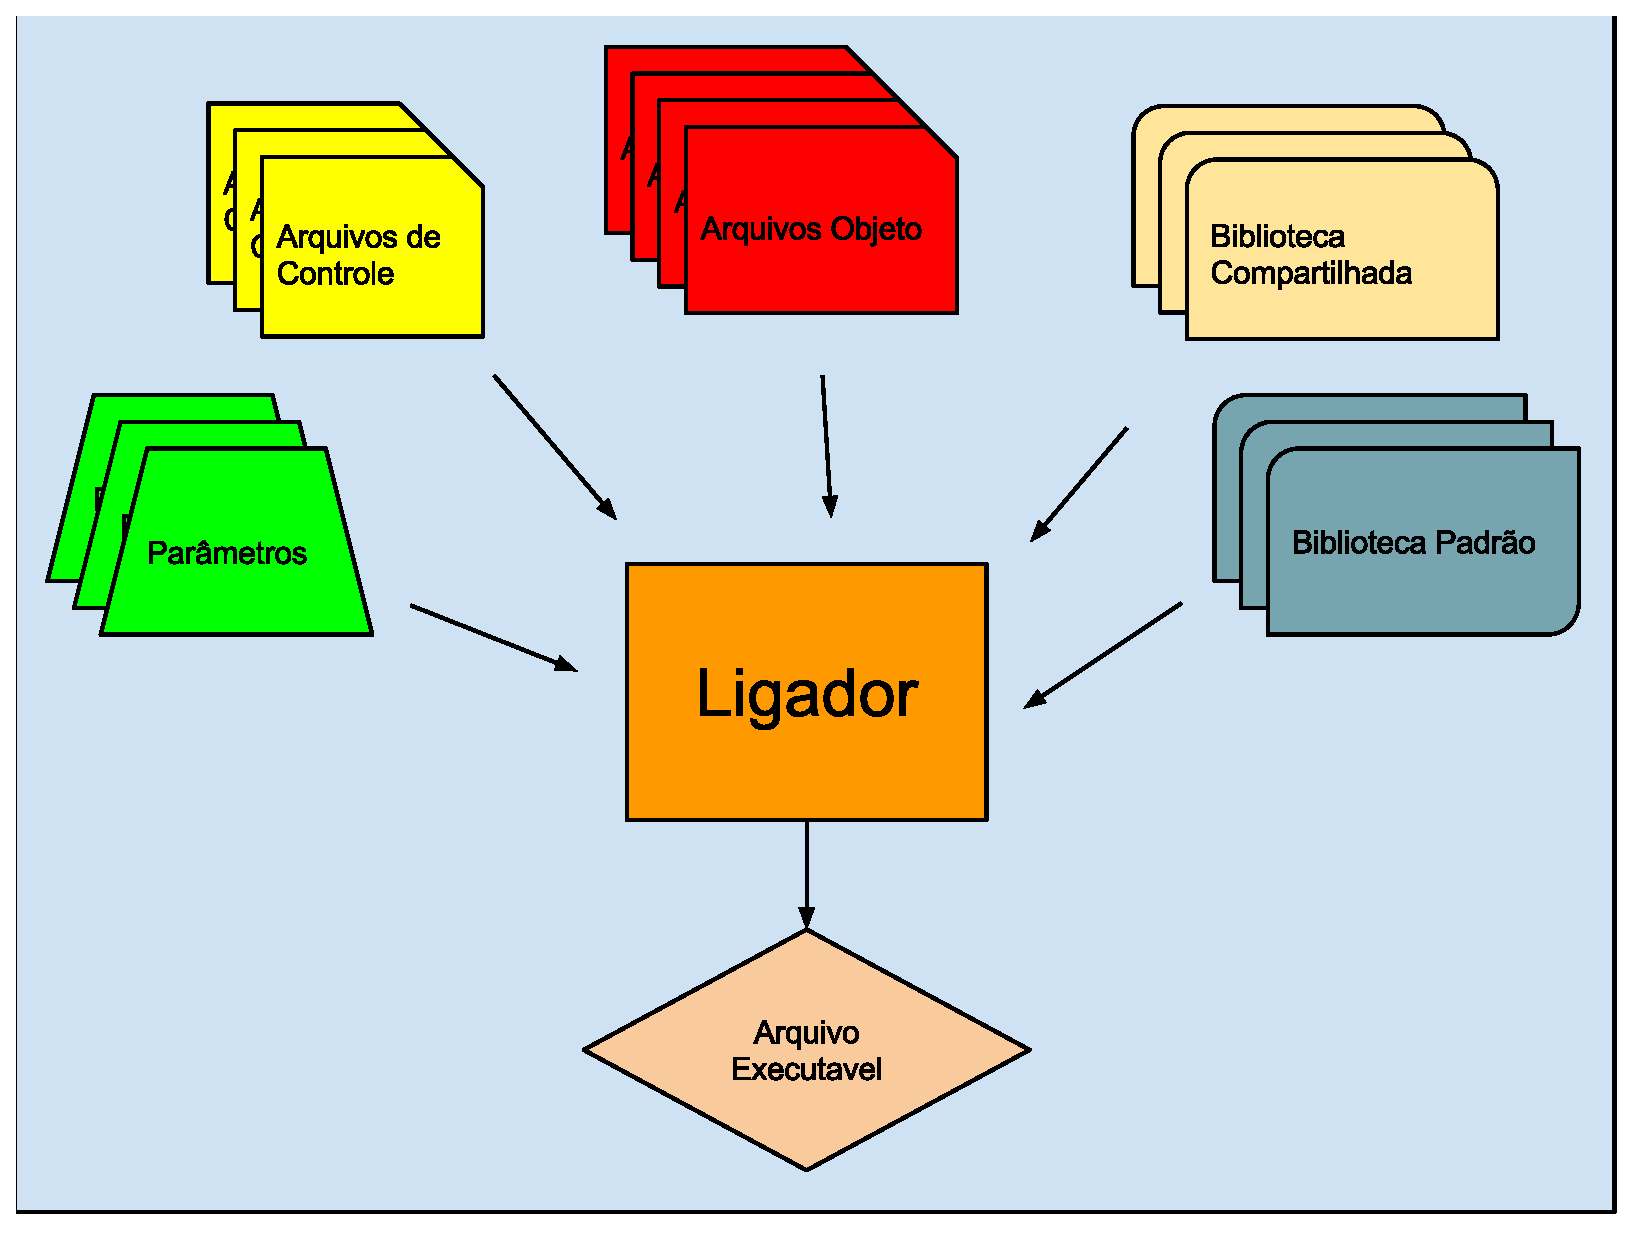
\includegraphics[keepaspectratio=true,scale=0.6]{figuras/ligador.eps}
    \caption{Representação da ligação entre objetos,(Levine,
											    John R.,2000),com adaptações.}
    \label{fig03}
\end{figure}

Um compilador é capaz de realizar a compilação de partes de programas e gerar
 objetos que podem ser combinados para formar um programa executável. 
\textit{Linker} (ou Ligador) é um programa capaz de realizar a junção 
de objetos gerados por um compilador, ligando nomes mais abstratos em nomes
 mais concretos, permitindo o desenvolvedor escrever códigos usando nomes 
mais abstratos \cite{ref36}.


 Basicamente o Linker liga um nome ou simbolo escrito por um desenvolvedor e
 referencia a localização do inicio do código que possui a função ou o dado
 estático. Como no exemplo descrito por John Levine, o linker pega um 
referência escrita como “getline”  e vincula a “uma localização de 612 bytes 
no inicio de um código executável do modulo iosys” \cite{ref36}. 

A fase de linkedição existem dois passos. No primeiro o Linker recebe como 
entrada um conjunto de arquivos objetos, bibliotecas e parâmetros e produz
 como resultado um arquivo de saída, como mostrado na Figura \ref{fig03}
 \cite{ref37}. Neste passo é criada uma tabela com 
todos os segmentos definidos nos arquivos fontes e uma tabela de símbolos 
importados ou exportados. Depois o Linker atribui uma localização numérica 
para cada símbolo, determinando o tamanho e a localização dos segmentos no
 espaço de endereço final. O segundo passo usa as informações do primeiro
 para controlar a linkedição, ajustando os endereços de memória do código e
 escrevendo os endereços de código realocado no arquivo de saída
 (programa executável).


\subsection{Bibliotecas}

Com o passar do tempo utilizando compiladores e linkers, muitos 
desenvolvedores perceberam que poderiam economizar tempo e esforço 
reutilizando pedaços de códigos escritos em outros programas. Para evitar a
 cópia de arquivos entre projetos surgiram as chamadas bibliotecas \cite{ref38}.

Biblioteca é um conjunto de códigos compilados que podem ser incorporados a
 um ou mais de um projetos, como mostrado nas Figura \ref{fig04}, e figura
 \ref{fig05}. A organização de códigos em bibliotecas permite que 
programas sejam mais modulares, mais rápidos de recompilar e mais 
fáceis de manter\cite{Lasca}.

As bibliotecas podem ser divididas em três tipos: estáticas, 
dinâmicas e compartilhadas\cite{Lasca}.

\begin{figure}[h]
    \centering
        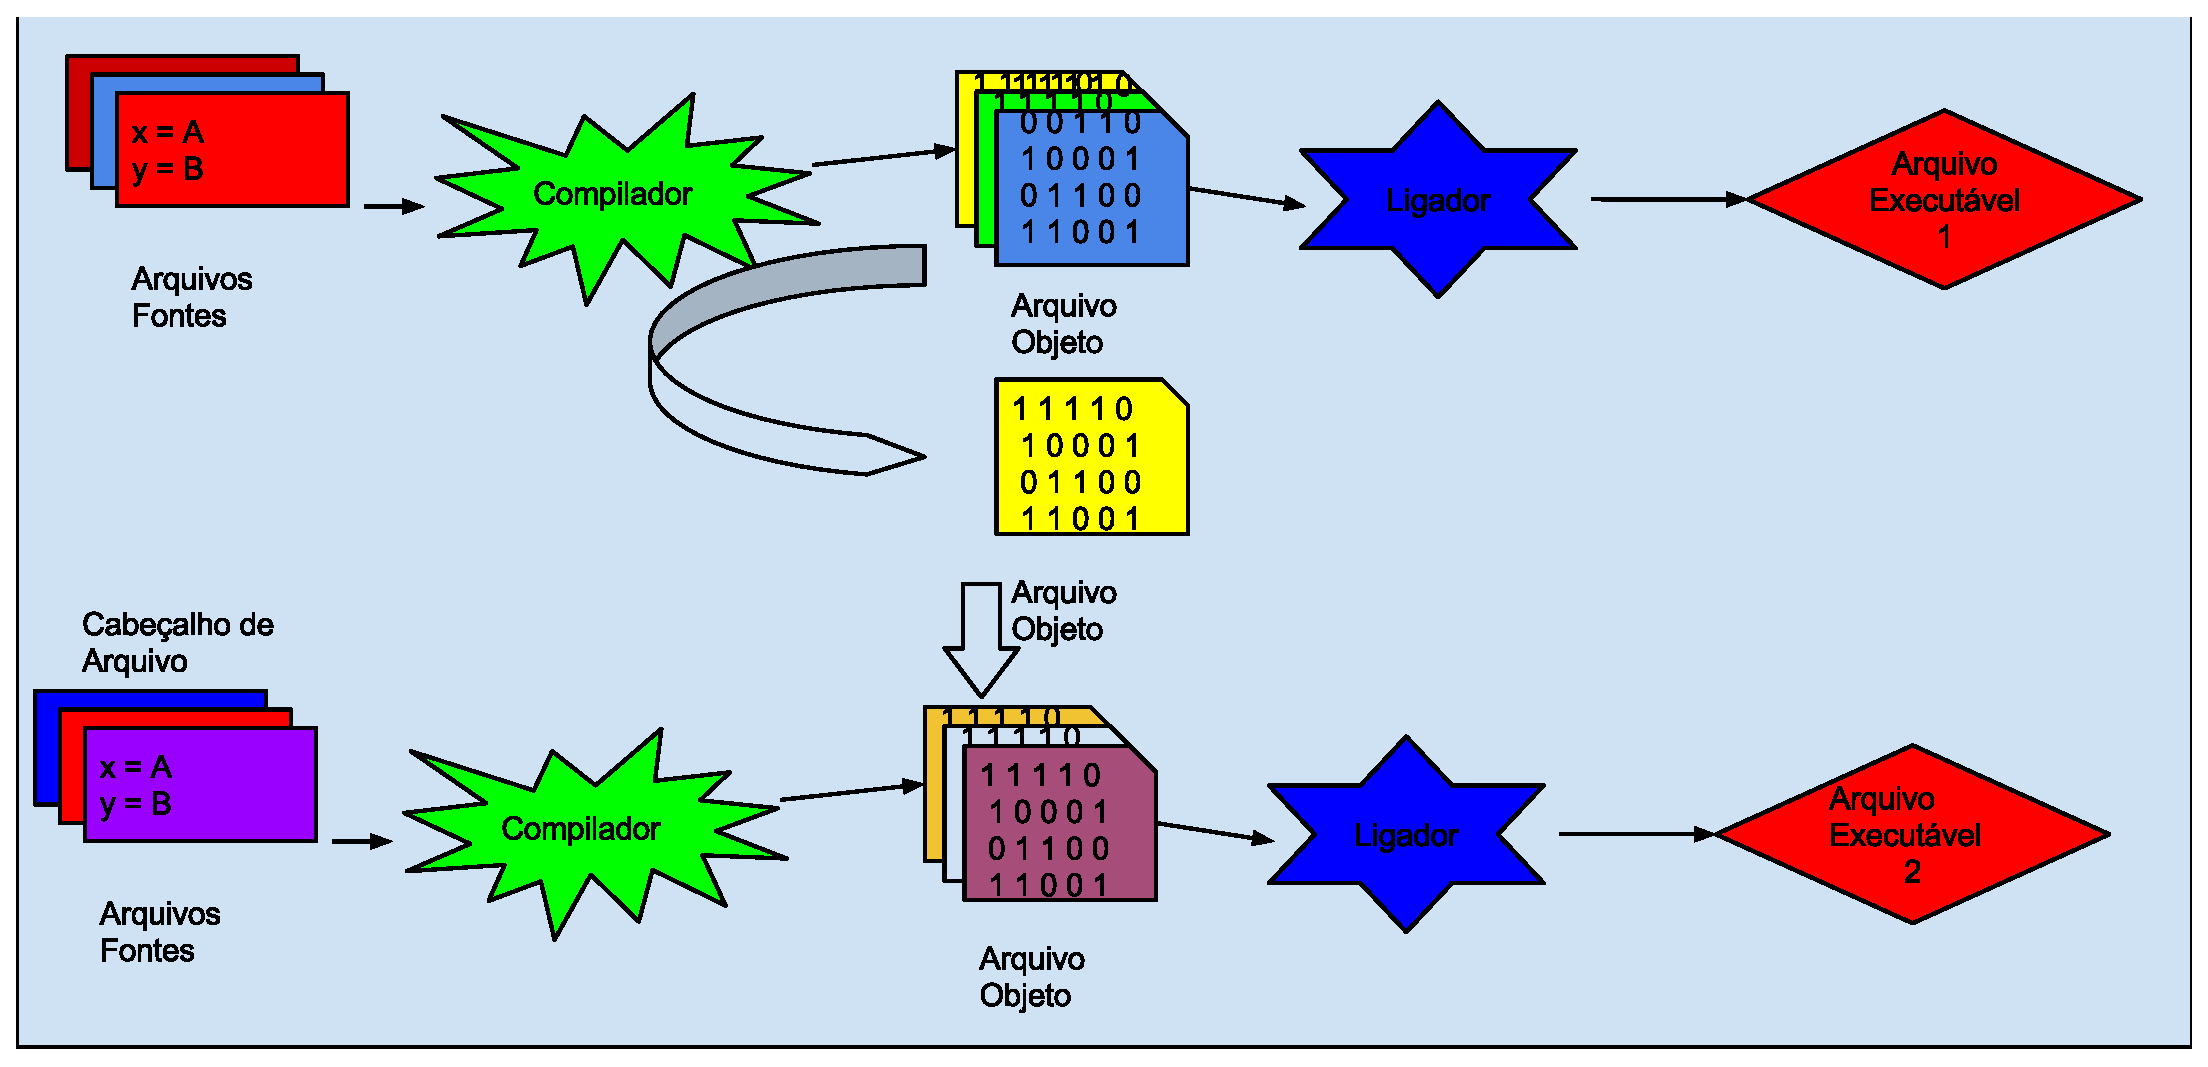
\includegraphics[keepaspectratio=true,scale=0.45]{figuras/reuso_lib_estatica.eps}
    \caption{ Representação de reuso com biblioteca estática,(Milan Stevanovic),com adaptações.}
    \label{fig04}
\end{figure}

\begin{figure}[h]
    \centering
        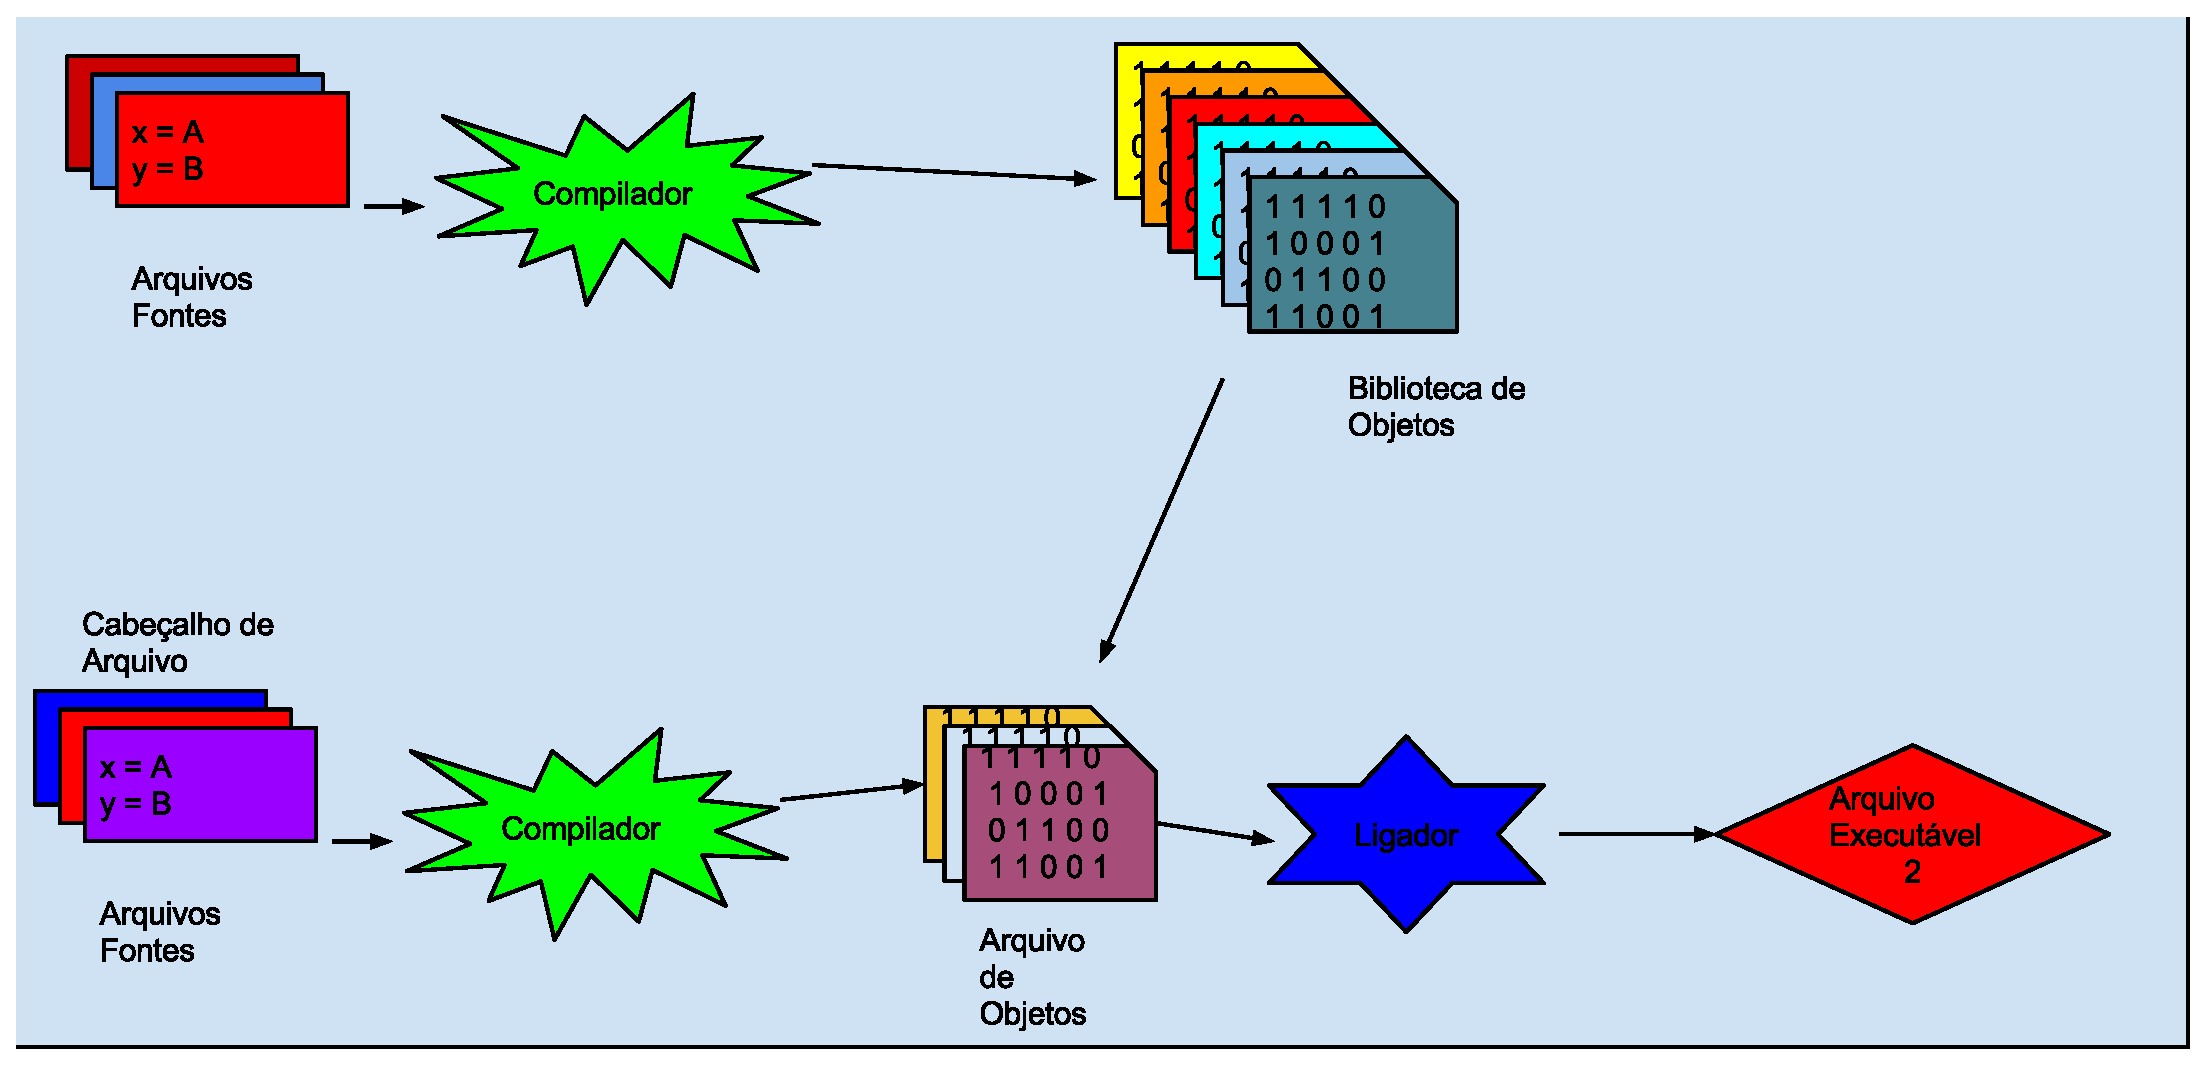
\includegraphics[keepaspectratio=true,scale=0.45]{figuras/reuso_lib_estatica2.eps}
    \caption{Representação de reuso (maneira trivial),(Milan Stevanovic),com adaptações.}
    \label{fig05}
\end{figure}


\subsection{Bibliotecas Estáticas}

Bibliotecas estáticas (que normalmente  são nomeadas com o  sufixo ‘.a’) 
são módulos de programas compilados separadamente, que podem ser utilizados
 na construção de um programa executável. Assim, após a etapa de compilação de
 um projeto, o linker faz a ligação entre as bibliotecas estáticas como
 mostrado na Figura \ref{fig04} \cite{ref39}.

Estas bibliotecas são mais difíceis de se manter, pois a cada atualização de uma
 biblioteca estática todos os projetos dependentes da mesma devem ser recompilados.
 Outra dificuldade é que um o binário final do projeto fica maior em relação aos
 outros tipos de bibliotecas (pois ele incorpora uma cópia de cada biblioteca
 estática utilizada) e pode conter informações que não são utilizadas no projeto.
 Bibliotecas estáticas, por estes motivos, não são utilizadas com tanta
 frequência nos dias de hoje.


\subsection{Bibliotecas Dinâmicas}

Ao contrário das bibliotecas estáticas, as bibliotecas dinâmicas são códigos
 objetos que podem ser carregados durante a execução de um projeto, como
 representado na figura \ref{fig06} \cite{ref41}. Bibliotecas dinâmicas 
não aumentam o tamanho do código binário do projeto final mas, no entanto,
 a execução do projeto necessita da utilização de um arquivo externo
 (normalmente nomeado com o sufixo ‘.so’ ou ‘.dll’), que contém as
 informações a serem carregadas\cite{Lasca2}. Em ambiente Linux as
 bibliotecas devem ser  registradas em uma variável de ambiente chamada
 LD\_LIBRARY\_PATH, que possui o caminho de todas as bibliotecas dinâmicas
 que podem ser utilizadas.

\begin{figure}[h]
    \centering
        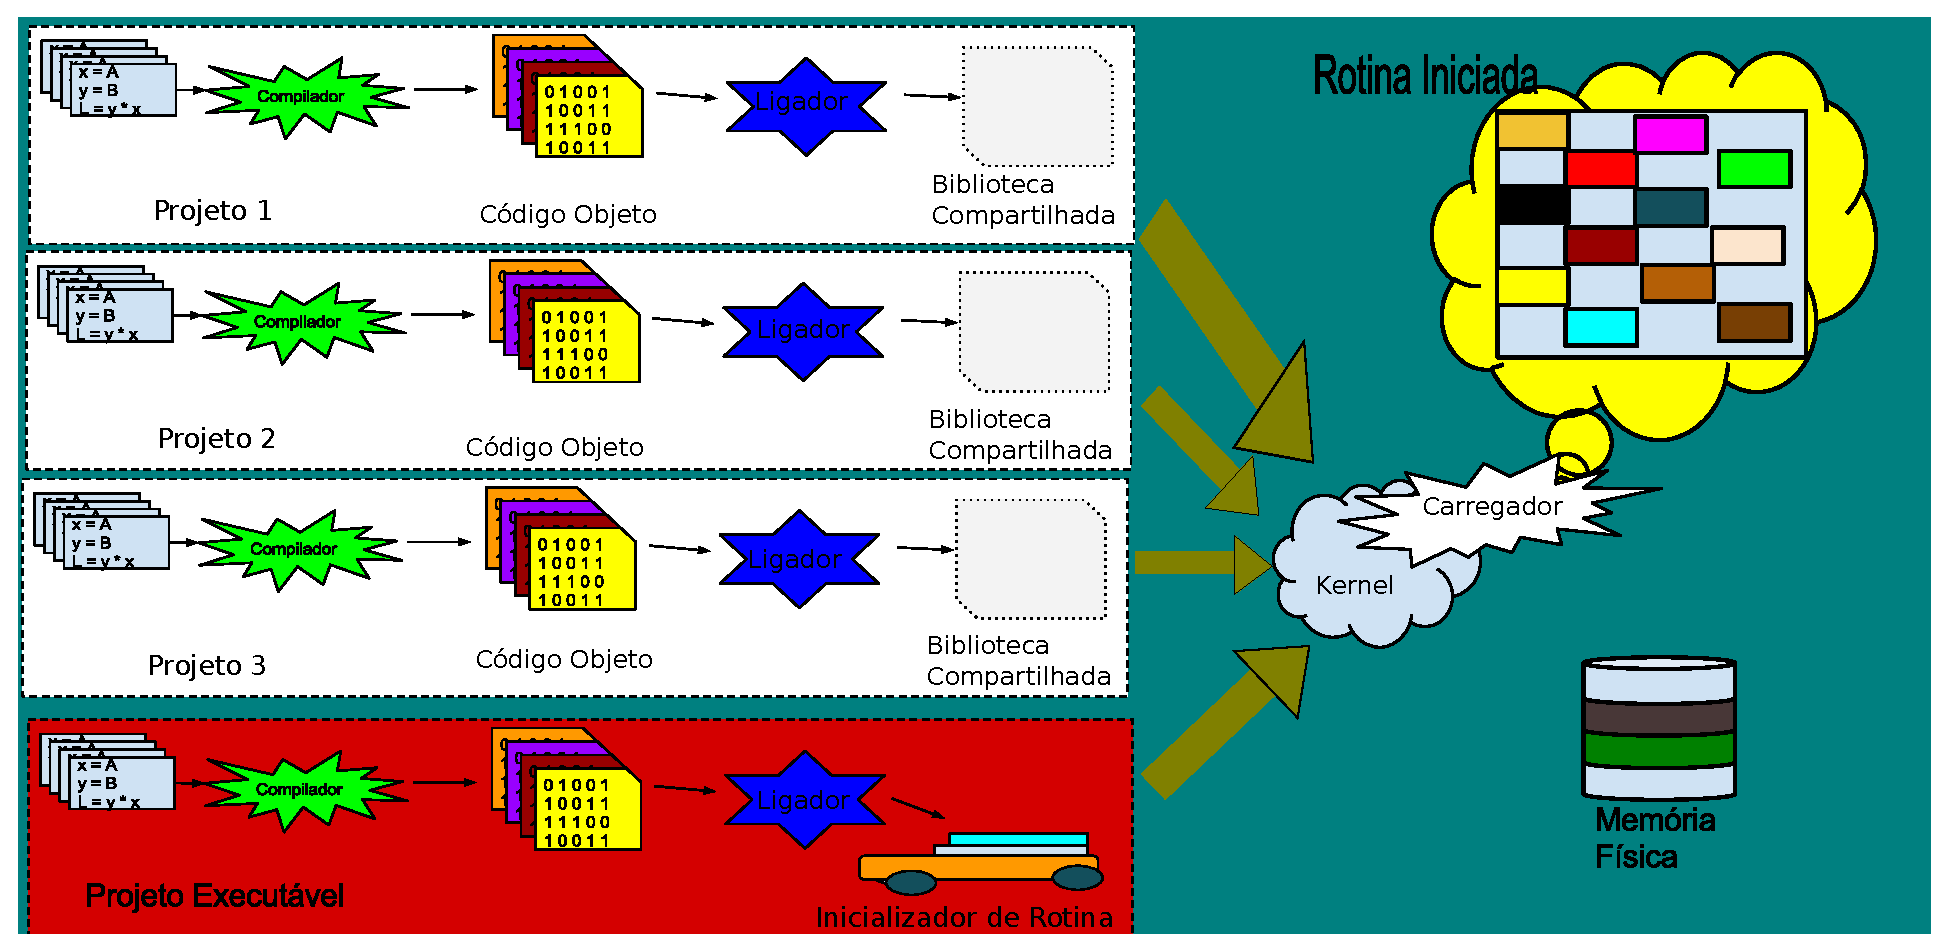
\includegraphics[keepaspectratio=true,scale=0.5]{figuras/dynamic_lib.eps}
    \caption{Representação de biblioteca dinâmica,(Milan Stevanovic) com adaptações.}
    \label{fig06}
\end{figure}


\section{Métodos para a redução do tempo de compilação}

\subsection{Include Guards}\label{include_guards_section}

Em C++ a inclusão de um arquivo de código fonte em outro arquivo fonte é feita
 através da diretiva de pré-processamente chamada \texttt{include}, que pode 
ser utilizada como mostrado no Codigo \ref{codigo_04}. 

\begin{lstlisting}[language=C++,frame=single,captionpos=b,caption={Diretiva de 
                           pré-processamento para inclusão de um arquivo},
                                                   label=codigo_04]
// biblioteca de sistema 
#include <nome do arquivo>  

ou

// outras bibliotecas 
#include "nome do arquivo"  

\end{lstlisting}


Diretivas \texttt{include} normalmente são utilizadas várias vezes em um projeto.
 No entanto, o pré-processador não é capaz de verificar se um arquivo já foi
 adicionado, o que pode ocasionar um erro de duplicação de definição de
 estruturas e elementos do código. Um exemplo deste problema é mostrado na
 Figura \ref{fig07} \cite{ref41}.

\begin{figure}[h]
    \centering
        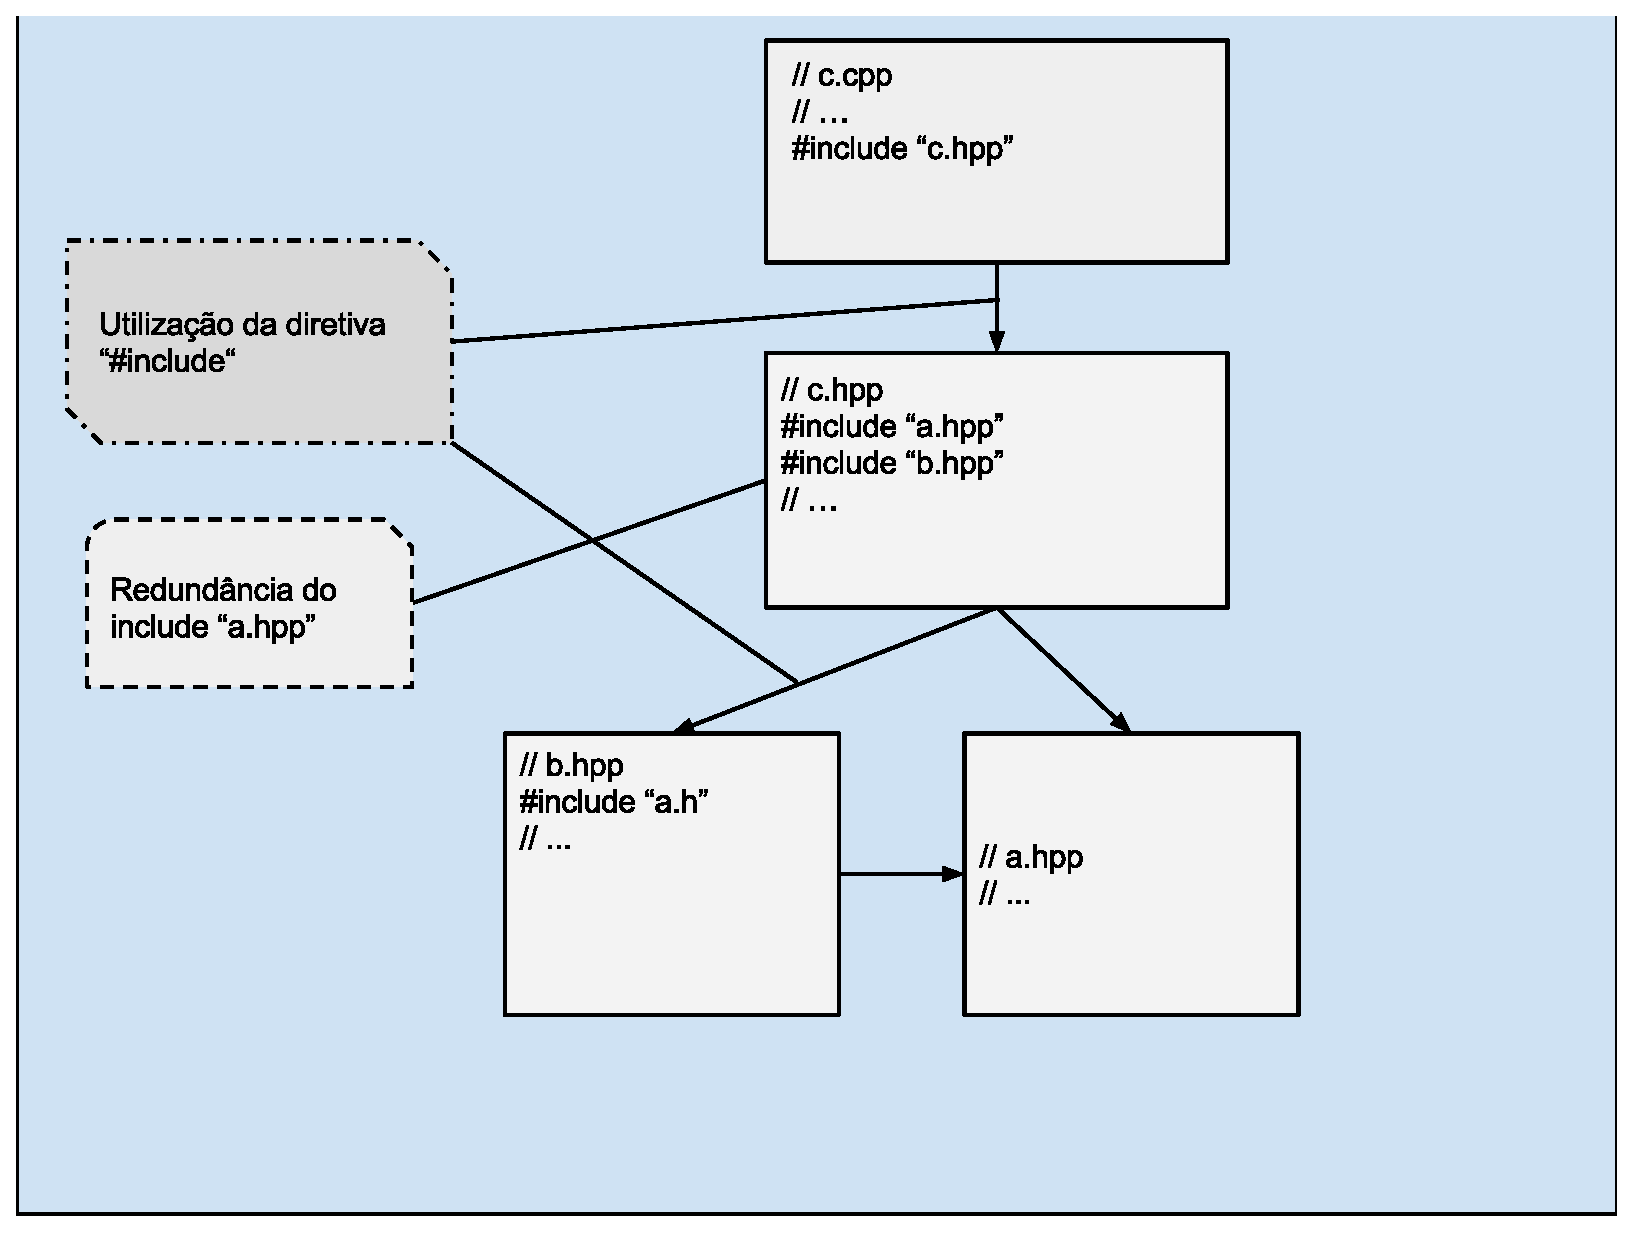
\includegraphics[keepaspectratio=true,scale=0.6]{figuras/multi_include.eps}
    \caption{ Representação de includes redundante,(John Lakos,1996) com adaptações.}
    \label{fig07}
\end{figure}

Para correção deste problema foram criadas as guardas de inclusão 
(no inglês chamada de  \textit{include guards} ou \textit{guard conditions}),
 que são diretivas de pré-processamento utilizada para verificar se um
 identificador já está definido ou não. Existem varias versões de guardas
 de inclusão, as quais serão citadas adiante\cite{ref42}.

Normalmente, arquivos-cabeçalho (ou \textit{headers}) são utilizados para
 declarações de estruturas, variáveis, funções e macros. Tais arquivos são
 identificados pelos sufixo ‘.h’,’.hpp’,’.hxx’ ou ‘.hpp’. As implementações
 das funções e definições de variáveis são feitas, na maioria das vezes, em
 arquivos denominados fontes (ou \textit{sources}), cujas extensões mais
 comuns são ".c", ".cpp", ".cxx", ".cc", ".c++", entre outros
 \cite{gcc-sufix}.

Há quatro tipos de guardas de inclusão:

\begin{enumerate}
\item Interna ao arquivo \textit{header}:

A diretiva "\#ifndef" é utilizada para verificar se um identificador foi 
 definido (forma negativa, para a forma positiva a diretiva é "\#ifdef"); a 
diretiva "\#define" é utilizada para definir um identificador; e a diretiva 
"\#endif" e utilizada para finalizar  uma condição (diretivas "\#ifdef" e 
"\#ifndef") \cite{ref42}.

Caso o identificador já esteja definido, o pré-processador irá ignorar 
qualquer informação que que esteja entre as diretivas "\#ifndef"  e "\#endif";
 caso não esteja definido, o identificador serão então definido e as informações
 que seguem a diretiva serão incluídas no arquivo resultante\cite{ref42}.

Os Códigos \ref{codigo_004}, \ref{codigo_05} e \ref{codigo_06} ilustram uma 
guarda de inclusão interna ao arquivo \textit{header}.

\begin{lstlisting}[language=C++,frame=single,captionpos=b,caption={
									Arquivo c.hpp contendo guardas
													 de inclusão interna},
                                                            label=codigo_004]
// c.h  declaracao de variavel
// verficar se o simbolo INCLUDE_C esta definido
#ifndef INCLUDE_C   
// define um simbolo INCLUDE_C
#define INCLUDE_C   

#include "a.hpp"      // importa o arquivo "a.hpp"
#include "b.hpp"      // importa o arquivo "b.hpp"

...                 // define as estruturas

#endif              // fim da condicional "#ifndef" 
\end{lstlisting}

\begin{lstlisting}[language=C++,frame=single,captionpos=b,caption={
                                     Arquivo b.hpp que inclue o arquivo a.h},
                                                            label=codigo_05]
// b.hpp
#ifndef INCLUDE_B
#define INCLUDE_C
 #include "a.hpp"
 // declaracao de estruturas 
 ...
#endif    
\end{lstlisting}

\begin{lstlisting}[language=C++,frame=single,captionpos=b,caption={Arquivo a.hpp 
                                    contendo guardas de inclusão interna},
                                                            label=codigo_06]
// a.hpp    arquivo de declaracao
#ifndef INCLUDE_A
#define INCLUDE_A
  // declaracao de estruturas 
  ...
#endif
\end{lstlisting}


\item Externa ao arquivo de \textit{header}:
 
Na  guarda de condição externa  são utilizadas as mesmas diretivas da interna,
 sendo a única diferença é a localização das diretivas: elas antecederão o uso
 da diretiva \#\texttt{include}. Um exemplo da utilização de guarda de condição 
externa é mostrado nos Código \ref{codigo_07},\ref{codigo_08} e
 \ref{codigo_09}\cite{ref42}.


\begin{lstlisting}[language=C++,frame=single,captionpos=b,caption={
									Arquivo c.hpp 
                                    contendo guardas de inclusão externa},
                                                            label=codigo_07]
// c.hpp arquivo de declaracao de estruturas de c

#ifndef INCLUDE_A
#define INCLUDE_A
/* inclue o arquivo a.hpp caso o simbolo 
   INCLUDE_A nao esteja definido */
#include "a.hpp"
#endif
        
#ifndef INCLUDE_B
#define INCLUDE_B
 /* inclue o arquivo b.hpp caso o simbolo 
    INCLUDE_B nao esteja definido */
 #include "b.hpp"
#endif

 ... //implementa as declaracoes

\end{lstlisting}

\begin{lstlisting}[language=C++,frame=single,captionpos=b,caption={
										   Arquivo a.hpp 
                                           com guarda de inclusão externa},
                                                            label=codigo_08]
// a.hpp         declaracao das estruturas de a.hpp

...

\end{lstlisting}

\begin{lstlisting}[language=C++,frame=single,captionpos=b,caption={
										   Arquivo b.hpp
                                           com guarda de inclusão externa},
                                                            label=codigo_09]
//b.hpp        declaracao das estruturas de b.hpp

...

\end{lstlisting}


\item Redundância:\label{redundancia_melhor}

Consiste em utilizar, simultaneamente, as guardas de inclusão internas e 
externas. 

Segundo John Lakos, está guarda de inclusão é a mais trabalhosa de ser mantida
 mas, no entanto, é a que mais reduz o tempo de compilação de um projeto. Ele
 realizou um experimento utilizando guardas de inclusão com e sem redundância,
 e obteve os resultados mostrados nas Tabelas \ref{tab:tabela_01} e 
\ref{tab:tabela_02};

\begin{table}
    \centering
    \begin{tabular}{ |c | c | c | c |}
    \hline
    Quantidade de Arquivos & SEM & COM & Sem Redundancia/Com Redundancia\\
    \hline
    1 & 0.2 & 0.2 & 1.0\\
    \hline
    2 & 0.2 & 0.2 & 1.0\\
    \hline
    4 & 0.3 & 0.3 & 1.0\\
    \hline
    8 & 0.5 & 0.3 & 1.67\\
    \hline
    16 & 0.7 & 0.4 & 1.75\\
    \hline
    32 & 1.5 & 1.1 & 3.0\\
    \hline
    64 & 0.2 & 0.2 & 1.0\\
    \hline
    128 & 25.9 & 3.5 & 74.0\\
    \hline
    256 & 126.5 & 13.6 & 9.3\\
    \hline
    512 & 702.3 & 61.6 & 11.4\\
    \hline
    1024 & 4378.5 & 306.6 & 14.28\\
    \hline
    \end{tabular}
    \caption {Amostra de Redundância com 10 headers por linha}
    \label{tab:tabela_01}
\end{table}

\begin{table}[h]
    \centering
    \begin{tabular}{ |c | c | c | c |}
    \hline
    Quantidade de Arquivos & SEM & COM & Sem Redundância/Com Redundância\\
    \hline
    1 & 0.2 & 0.2 & 1.0\\
    \hline
    2 & 0.2 & 0.2 & 1.0\\
    \hline
    4 & 0.4 & 0.3 & 1.33\\
    \hline
    8 & 0.7 & 0.4 & 1.75\\
    \hline
    16 & 1.7 & 0.5 & 3.4\\
    \hline
    32 & 5.8 & 0.9 & 6.44\\
    \hline
    64 & 22.1 & 2.0 & 11.05\\
    \hline
    128 & 89.5 & 5.2 & 17.21\\
    \hline
    256 & 376.5 & 17.1 & 22.02\\
    \hline
    512 & 1697.4 & 68.6 & 24.74\\
    \hline
    1024 & 8303.8 & 330.6 & 25.12\\
    \hline
    \end{tabular}
    \caption {Amostra de Redundância com 100 headers por linha }
    \label{tab:tabela_02}
\end{table}

\item Pragma Once

Pragma once é uma diretiva de pré-processamente que possui o objetivo de
 garantir que um arquivo será lido apenas uma vez: caso uma diretiva 
"\#include" seja utilizada novamente e o arquivo já foi incluído anteriormente,
 o mesmo não será aberto. No entanto, esta implementação se tornou obsoleta 
 na implementação do gcc \cite{gcc-pragma_once}. Os Códigos \ref{codigo_10} 
, \ref{codigo_11} e \ref{codigo_12} exemplificam o uso desta diretiva.



\begin{lstlisting}[language=C++,frame=single,captionpos=b,caption={
                                    Exemplo de arquivo c.hpp com guarda de 
                                         inclusão que utiliza \#pragma once},
                                                            label=codigo_10]
// c.hpp
/* pragma once indicar que o 
   arquivo c.hpp sera
   incluido apenas 1 vez */
#pragma once            
#include "a.hpp"
#include "b.hpp"

 // declaracoes de c.hpp

 ...

\end{lstlisting}

\begin{lstlisting}[language=C++,frame=single,captionpos=b,caption={
                                   Exemplo de arquivo a.hpp com guarda de 
                                    inclusão que utiliza \#pragma once},
                                                            label=codigo_11]
// a.hpp
#pragma once 

 // declaracoes de a.hpp

 ...

\end{lstlisting}

\begin{lstlisting}[language=C++,frame=single,captionpos=b,caption={ 
                                   Exemplo de arquivo b.hpp com guarda de 
                                      inclusão que utiliza \#pragma once},
                                                            label=codigo_12]
//b.hpp
#pragma once 

 // declaracoes de b.hpp

 ...

\end{lstlisting}

\end{enumerate}

\subsection{Forward Declaration}\label{forward_declaration_section}

Em C++, todas as entidades (variáveis, funções, classes, estruturas, uniões,
 etc) deve sem declaradas ou definidas antes de serem referenciadas. Definir
 uma classe antes dela ser utilizada não é possível quando as duas classes
 diferentes referenciam uma a outra, gerando uma referência cíclica
\cite{ref43}.

Considere um exemplo de duas classes, Doutor e Paciente,apresentadas no 
Código \ref{codigo_13}. Neste exemplo, a classe Doutor requer a 
declaração ou definição da classe Paciente, e a classe Paciente necessita 
de uma declaração ou de uma definição da classe Doutor. Desta forma, a 
compilação geraria um erro, pois antes de utilizar uma referência é 
necessário declarar ou definir esta referência.

\begin{lstlisting}[language=C++,frame=single,captionpos=b,caption={
                        Implementação de classes Paciente e Doutor},
                                                     label=codigo_13]
// doutor_paciente.cpp

class Doutor {

  // implementacoes privadas
  private:

  /* a classe Doutor necessita saber que existe 
     a referencia para a classe Paciente */
  Paciente* p; 

  ...          

  // implementacoes publicas
  public:

  ...	

};

class Paciente {

 // implementacoes privadas
 private:

 /* a classe paciente necessita saber que 
 existe a classe Doutor, no entanto
 doutor so existe se souber da referencia
 de paciente */
 Doutor * d; 

 ...  

 // implementacoes publicas
 public:

 ...  

};

\end{lstlisting}

Para resolver este problema é preciso utilizar uma 
referência incompleta (\textit{"forward"}) da classe Doutor e da
 classe Paciente, conforme apresentado no Código \ref{codigo_14}. 

\begin{lstlisting}[language=C++,frame=single,captionpos=b,caption={ 
								Implementação de classes Paciente e
							 Doutor utilizando forward declaration},
                                                    label=codigo_14]
// forward declaration
class Doutor;   
class Paciente; 

class Doutor   {
  // implementacoes privadas
  private:

  /* a referencia incompleta de Paciente existe,
   entao Doutor pode armazenar a 
   referencia do paciente */

  Paciente* p; 
  
  ... 

  // implementacoes publicas
  public: 

  ...
 
};

class Paciente {
  // implementacoes privadas
  private:
	
  Doutor * d; 

  ... 
	
  // implementacoes publicas
  public: 

  ...

};

\end{lstlisting}

A declaração incompleta (\textit{forward declaration}) de uma classe somente podem
 ser utiliza em arquivos na forma de ponteiro (utilizando o operador "*")
 ou referência (utilizando o operador "\&"), pois estas não requerem uma
 definição de classe completa porque, em C++, é alocado uma quantidade fixa
 de armazenamento para estes tipos de variáveis \cite{ref43}.

Um exemplo incorreto de utilização de forward declaration seria utilizar
 um construtor da classe Doutor é mostrado no Código \ref{codigo_15}.


\begin{lstlisting}[language=C++,frame=single,captionpos=b,caption={
                   Uso incorreto de Forward Declaration},
                                                label=codigo_15]
   // forward declaration
   class Doutor;

   // utilizacao da estrutura Doutor
   Doutor doutor();

\end{lstlisting}

Como já mencionado, qualquer entidade deve ser declarada ou definida antes
 de ser utilizada, então o caso acima é válido para funções, variáveis,
 estruturas e uniões, entre outros. A Tabela \ref{tab:tabela_03} mostra
 um exemplo de \textit{forward declaration} para alguns destes tipos
 de estruturas.

\begin{table}[h]
    \centering
    \begin{tabular}{ |c | c |}
    \hline
    Definição & Declaração\\
    \hline
    int x; & extern int x;\\
    \hline
    typedef struct Foo{int x;}; & typedef struct Foo;\\
    \hline
    class Foo { int x;public: Foo() ... }; & class Foo;\\
    \hline
    int Add( int x ,int  y) { return x + y; } & int Add(int x, int y);\\
    \hline
    union Foo { int x; char x; }Foo; & union Foo;\\
    \hline
    \end{tabular}
    \caption{Exemplos de \textit{forward declaration}}
    \label{tab:tabela_03}
\end{table}


Na linguagem C++ há uma separação entre  a implementação e a interface de
 classe\cite{ref44}.Na maioria dos casos, a definição de uma classe possui
 detalhes de sua implementação, como nos Código \ref{codigo_16} e \ref{codigo_17}.


\begin{lstlisting}[language=C++,frame=single,captionpos=b,caption={ 
                          Arquivo declaração da classe Pessoa },
                                                label=codigo_16]

// pessoa.hpp   - declaracao da classe
#ifndef PESSOA_HPP
#define PESSOA_HPP

// conhecer detalhes de implementacao da string
#include <string>       
// conhecer detalhes de implementacao da Data
#include "data.hpp"     

class Pessoa{
public:

  Pessoa(std::string nome,Data data);
  std::string meu_nome() const;
  Data meu_aniversario() const;

private:
  // detalhes de implementacao na declaracao
  std::string nome;        

  // detalhes de implementacao na declaracao
  Data aniversario;        
};

#endif

\end{lstlisting}

\begin{lstlisting}[language=C++,frame=single,captionpos=b,caption={
                               Arquivo definição da classe Pessoa},
                                                    label=codigo_17]
// pessoa.cpp implementacao da classe
#include "pessoa.hpp"

Pessoa::Pessoa(std::string nome, Data data)
        : nome(nome),aniversario(data)
{
}

std::string
Pessoa::meu_nome() const
{
        return nome;
}
Data
Pessoa::meu_aniversario() const
{
        return aniversario;
}

\end{lstlisting}    


Definir uma classe com detalhes de implementação em sua definição não é uma
 boa prática de programação, uma vez que ela não pode ser compilada sem
 conhecer as definições das classes utilizadas em sua implementação para
 realizar alocação de memória. Isso conduz à utilização da diretriz
 "\#include", gerando dependência entre arquivos\cite{ref44}.

Uma maneira de contornar este problema é utilizar uma forward declaration e a
 armazenar referências das classes, de modo que as definições das classes não
 possuam dependência uma das outras. Isto evita que definições de classes sejam
 modificadas com frequência e reduz a quantidade de recompilações devidas às
 dependência entre os  arquivos. Veja os Códigos \ref{codigo_18} 
e \ref{codigo_19}.


\begin{lstlisting}[language=C++,frame=single,captionpos=b,caption={ 
                         	     Arquivo definição da classe Pessoa,       
                          utilizando \textit{forward declaration}},
                                                label=codigo_18]
// pessoa.hpp 
#ifndef PESSOA_HPP
#define PESSOA_HPP

// header para string forward declaration
#include <bits/stringfwd.h>    

// forward declaration
class Data;            

class Pessoa{
public:
        Pessoa(std::string& nome,Data *data);
        std::string& meu_nome() const;
        Data* meu_aniversario() const;

private:
// referencia para string
  std::string& nome;

// referencia para Data
  Data* aniversario;
};

#endif

\end{lstlisting}


\begin{lstlisting}[language=C++,frame=single,captionpos=b,caption={ 
                          Arquivo definição da classe Pessoa,       
                      utilizando \textit{forward declaration} },
                                                label=codigo_19]

// pessoa.cpp -  implementacao
#include "pessoa.hpp"
#include <string>

Pessoa::Pessoa(std::string& nome, Data* data)
        : nome(nome),aniversario(data)
{
}
std::string&
Pessoa::meu_nome() const
{
        return nome;
}
Data*
Pessoa::meu_aniversario() const
{
        return aniversario;
}

\end{lstlisting}


O Código \ref{codigo_18} foi feito o uso da diretiva \#include
 <bits/stringfwd.h>. Em C++  existem arquivos-cabeçalhos que possuem a
 implementação de forward declaration. A Tabela \ref{tab:tabela_04} lista 
 alguns forward declaration que podem ser utilizados em C++ segundo
 a gcc-gnu \cite{gcc-api}.

\begin{table}[h]
    \centering
	\begin{tabular}{ |l|p{10cm} | l|p{10cm} |}
	\hline
	Biblioteca & Alguns includes do header\\
	\hline

	\#include<bits/stringfwd.h> & std::string,

								 std::wstring,std::u16string, 

								 std::u32string;\\
	\hline
	\#include <iosfwd> & std::filebuf, std::fstream,
						std::ifstream, std::iostream,
						std::istream, std::ofstream,
						std::ostream, std::ostringstream,
						std::stringbuf,std::streambuf,
						entre outros;\\
	\hline
	\#include <bits/localefwd.h> & std:has\_facet, std::isalnum,
								  std::isalpha, std::iscntrl,
								  std::isdigit,std::isgraph,
								  std::islower, std::isprint,
								  std::ispunct,
								  std::isspace,std::issuper,
								  entre outros;\\
	\hline
	\#include <bits/algorithmfwd.h> & std::adjacent\_find,std::any\_of,
									 std::binary\_search, 
									 std::copy\_backward, std::copy\_if,
									 std::count\_if, std::count,
									 std::find\_end, std::find\_if,
									 entre outros.\\
	\hline
	\end{tabular}
	\caption {Tabela de Algumas \textit{forward 
			  declaration} padrões do c++}
    \label{tab:tabela_04}
\end{table}


\subsection{MakeFile}\label{Makefile_section}


Make é uma ferramenta utilizada para determinar automaticamente quais
 os trechos de código de um grande projeto precisam serem recompilados
 após alguma iteração de desenvolvimento. Esta ferramenta foi implementada
 por Richard Stallman e Roland McGrath. Desde a versão 3.76 até os dias de
 hoje vem sendo mantida por Paul D.Smith\cite{Lasca2}.O manual de utilização do makefile
 é disponibilizado no portal GNU \cite{ref45}.

Para utilizar a ferramenta make é necessário a criação de um arquivo chamado
 makefile, que contem as descrições de relações entre os arquivos em um projeto
 e comandos necessários para realizar as atualizações em cada arquivo\cite{Lasca2}.
 Depois de definir o arquivo makefile, utiliza a chamada de sistema apresentada 
no Codigo \ref{codigo_20}.

\begin{lstlisting}[language=C++,frame=single,captionpos=b,caption={
                             Chamada de Sistema para executar o programa make},
				                                                label=codigo_20]
    $ make
\end{lstlisting}


O programa make realiza as devidas verificações nos códigos fontes e
 nos códigos objetos, e caso seja necessário recompilar um arquivo, o
 makefile contém as instruções necessárias para o tal procedimento
 \cite{ref46}.


\subsection{Estrutura básica de um arquivo makefile}

Arquivos makefile contém 5 tipos básicos de elementos: regras explicitas,
 regras implícitas, definição de variáveis, diretivas e comentários.

\begin{enumerate}

    \item Regras Explicitas: \
        conjunto de regras que informam quando e como refazer as construções
         de arquivos. Ela é definida pela estrutura apresentada no Codigo \ref{codigo_21}.


        \begin{lstlisting}[language=C++,frame=single,captionpos=b,caption={
                                     			Regras explicitas Makefile},
                                                        label=codigo_21]

alvo ... : pre-requisitos ... 
    procedimentos
	...
ou 

alvo ... : pre-requisitos ... ; procedimentos
    procedimentos
    ...

        \end{lstlisting}


 O \textbf{alvo} é utilizado para nomear os artefatos que devem ser gerados pelo projeto.
 O alvo também pode ser utilizado para fazer a chamada de execução de um trecho
 específico do Makefile,  sendo passando como parâmetro na utilização do comando
 make.

 Os \textbf{pré-requisitos} são os endereços de arquivos utilizados como entrada para a 
criação do alvo. Este campo é opcional, pois podem existir instruções que não
 necessitam de arquivos de entrada, como por exemplo a instrução "clean”
 (tipicamente utilizada para remoção de todos os códigos objetos gerados a partir
 dos códigos do projeto) \cite{ref47}.

Os \textbf{procedimentos} são as ações que devem ser executadas a partir do comando make.
Este bloco pode conter mais de um comando em uma linha, ou  vários comandos em
 linhas separadas \cite{ref47}.

    \item Regras Implícias: \
 conjunto de regras que informam quando e como refazer uma classe de arquivos
 baseadas em seus nomes e padrões \cite{ref48}. Um exemplo de utilização de 
 padrões é apresentado no Código \ref{codigo_22} \cite{ref49}
        
    \begin{lstlisting}[language=C++,frame=single,captionpos=b,caption={ 
                          Exemplo de utilização de padrões no Makefile},
                                                        label=codigo_22]

# gerar  objetos ".o" utilizando arquivos ".c"
%.o : %.c
    procedimentos
    ...

    \end{lstlisting}


    \item Definição de Variáveis:\
 é uma linha que especifica um valor para uma variável que pode ser substituída no
 texto posteriormente \cite{ref43}. Veja o Código \ref{codigo_23} para um exemplo de 
definição de variável.

    \begin{lstlisting}[language=C++,frame=single,captionpos=b,caption={ 
                                     Definição de variavel e utilização},
                                                         label=codigo_23]
objetos = main.o command.o display.o files.o\
          search.o utils.o

clean:
    rm $(objetos)
    \end{lstlisting}


    \item Diretivas: \
são instruções que indicam ao make ações especiais a medida que é realizada a leitura do
 arquivo Makefile \cite{ref43}. Estas instruções podem ser:

    \begin{itemize}
        \item Realizar a leitura de um outro makefile, através da diretiva include, seguida do nome do arquivo.
        \item Utilizar ou ignorar parte do makefile.\cite{ref43} O Código \ref{codigo_24} ilustra o uso desta diretiva. 


    \begin{lstlisting}[language=C++,frame=single,captionpos=b,caption={ 
                             Exemplo Make file com diretiva condicional},
                                                         label=codigo_24]

ibs_for_gcc = -lgnu
normal_libs =

foo: $(objects)
ifeq ($(CC),gcc)
$(CC) -o foo $(objects) $(libs_for_gcc)
else
$(CC) -o foo $(objects) $(normal_libs)
endif

    \end{lstlisting}

    \begin{itemize}
        \item \textbf{ifeq:} Diretiva que começa a condicional e especifica a 
    condição. Ela contém 2 argumentos, separados por virgula e entre parêntesis.
     Caso os argumentos forem iguais as linhas entre o \textbf{ifeq} e o
     \textbf{else} serão executadas, caso contrário serão ignoradas\cite{ref50}.

        \item \textbf{else:} Diretiva que marca o início das instruções a serem 
    executadas caso a condição do \textbf{ifeq} falhe. Esta diretiva é opcional\cite{ref50}.

        \item \textbf{endif:} Diretiva que finaliza a condição. 
    Toda diretiva condicional condição deve ser terminada com endif\cite{ref50}.
    \end{itemize}

    \item Definir variáveis com mais de uma linha. Com a utilização da diretiva define
 e  da diretiva endef é possível realizar a definição de uma variável em mais
 de uma linha \cite{ref51}. O Código \ref{codigo_25} ilustra esta situação.

    \begin{lstlisting}[language=C++,frame=single,captionpos=b,caption={
						Exemplo Make file com definição de variavel em
													  multiplas linhas},
														label=codigo_25]
bar= "BAR"
define two-lines =
echo foo
echo $(bar)
endef
all:
$(two-lines)
    
    \end{lstlisting}


    \end{itemize}

    \item Comentários: \
Em arquivos Makefile a utilização de caractere "\#" em uma linha faz com
 que todos o carateres que o sucederem sejam ignorados. Caso seja necessário
 a utilização deste o caractere basta precedê-lo com o caractere "\\" 
(barra invertida)\cite{ref48}.

\end{enumerate}


\subsection{Padrões de um arquivo makefile para ferramentas GNU}

    
Tendo como referência o manual do GNU Make \footnote{
Manual GNU-Make: http://www.gnu.org/software/make/manual/make.pdf 
}, Seção 15.6, existem padrões que podem ser utilizados em arquivo
 makefile. Alguns dos mais comuns são:

\begin{enumerate}
    \item \textbf{all}: instrução executada por default pelo makefile, 
realiza as verificações do arquivos de código fonte e faz atualizações
 nos códigos objetos, se necessário;
    \item \textbf{install}: chama o make all e copia os arquivos 
executáveis, bibliotecas, e os demais artefatos do projeto para os 
locais adequados, de acordo com as necessiddades do projeto;
    \item \textbf{uninstall}: deleta todos os arquivos copiados 
pelo comando make install;
    \item \textbf{clean}: deleta todos os arquivos e diretórios 
criados na construção do programa final.
    \item \textbf{distclean}: remover os arquivos que foram gerados
 por algum comando make file, seja na configuração, seja na
 construção de um programa.
    \item \textbf{info}: gera um arquivo de informações sobre o programa.
    \item \textbf{dist}: gera um arquivo tar cujo nome contém a versão e
o nome do projeto e  que inclui  todo o conteúdo do diretório atual.
    \item \textbf{check}: gera o programa  e realiza testes. 
    \item \textbf{installcheck}: gera o programa, instala e realiza testes.
    \item \textbf{installdirs}: cria  os diretórios onde os arquivos devem ser instalados.
\end{enumerate}


\subsection{Executando makefile}

Depois de gerado o arquivo makefile utilizando as regras descritas nas seções anteriores,
 o comando make pode ser utilizado para executar as regras descritas.
O comando make pode ser utilizado como mostrado no Codigo \ref{codigo_26} e conforme apresentado na Tabela \ref{tab:tabela_05}.


    \begin{lstlisting}[language=C++,frame=single,captionpos=b,caption={ 
                                     Definição de variavel e utilização},
                                                         label=codigo_26]
    
        $ make [opcoes] ... [Alvo]

    \end{lstlisting}


\textbf{Alvo}: é a instrução que será executada pelo makefile. 
A omissão deste parâmetro leva a execução do alvo "all".
    
\textbf{Opções}: são flags de controle utilizadas pelo utilitario make.
 Exemplos de flags estão definidas na Tabela \ref{tab:tabela_05}:

\begin{table}[h]
    \centering
    \begin{tabular}{ | l|p{10cm} | l|p{10cm} |}
    \hline
    Flag & Descrição\\
    \hline
    -C dir , --directory=dir & Modifica o diretório antes de fazer a leitura do makefile\\
    \hline
    -f file    ,     --file=file     ,  --makefile=FILE & Realiza a leitura de um makefile especifico\\
    \hline
    -i   ,     --ignore-errors & Ignora erros na reconstrução de arquivos\\
    \hline
    -I dir   ,   --include-dir=dir & Especifica o diretório que inclue os makefiles\\
    \hline
    -j [jobs]  , --jobs[=jobs] & Especifica a quantidade de threads
                                 que podem ser executadas em paralelo. 
                                 Caso não seja passado a quantidade de
                                 threads ele não terá limites na criação
                                 de threads.\\
    \hline
    \end{tabular}
    \caption {Exemplos de flags que podem ser utilizadas no make}
    \label{tab:tabela_05}
\end{table}

    * Palavras entre "[" e "]" são opcionais.

\chapter[Metodologia]{Metodologia}


Este capítulo foi elaborado para melhorar o entendimento das atividades
 realizadas para a produção deste trabalho. O fluxo da Figura 
\ref{fig:fases_metodologia} define estas atividades.

\begin{figure}[h]
    \centering
        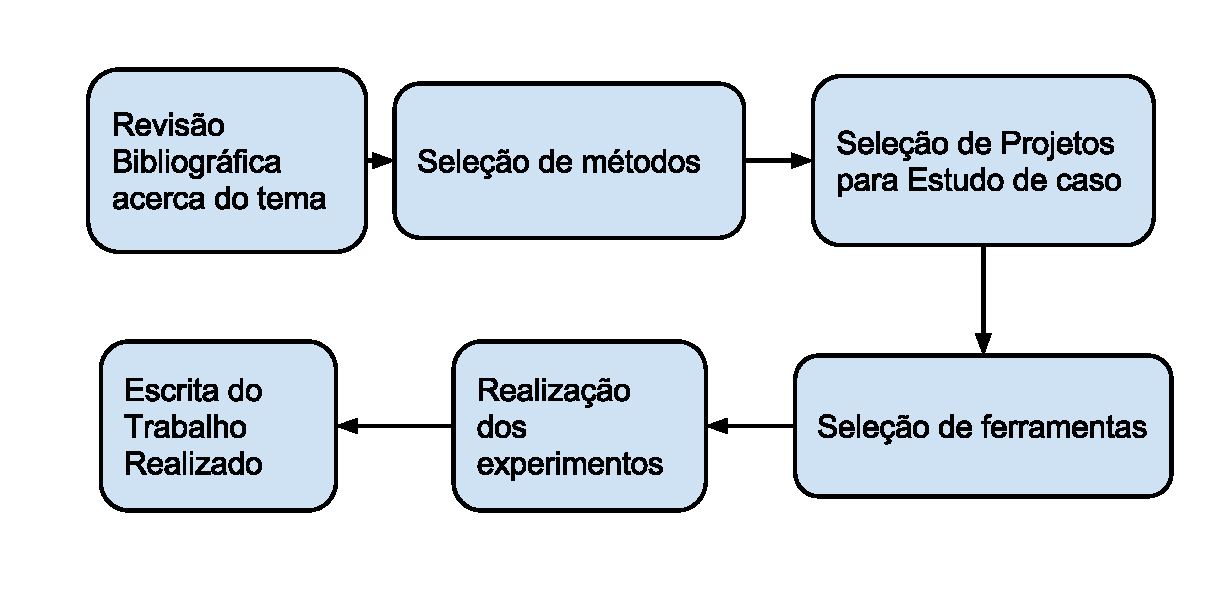
\includegraphics[keepaspectratio=true,scale=0.7]{figuras/fases_metodologia.eps}
    \caption{Fluxo de Atividades para a resolução destes trabalho}
    \label{fig:fases_metodologia}
\end{figure}


\section{Revisão Bibliográfica}

A revisão bibliográfica foi a primeira atividade realizada para a construção
 deste trabalho. Foi feito um estudo e levantamento de métodos, técnicas e
 ferramentas que podem auxiliar o desenvolvimento deste trabalho, além de
 elucidar a viabilidade da realização do mesmo. Esta revisão foi utilizada
 como referência para a  escrita da fundamentação teórica.

\section{Seleção de Métodos}

Para seleção de métodos foi realizada uma priorização dos métodos, técnicas e
 ferramentas encontradas durante a revisão bibliográfica. A priorização levou
 em conta o esforço da implementação/execução dos métodos, o tempo para a
 montagem de cada caso e o recurso computacional necessário para a criação
 destes.

Os métodos selecionados foram:

\begin{itemize}
	\item \textit{Include Guards}, descrito na Seção
 \ref{include_guards_section};
	\item \textit{Forward Declaration}, descrito na Seção
 \ref{forward_declaration_section};
	\item Makefile, descrito na Seção
 \ref{Makefile_section};
	\item Otimização de baixo nível descrito na Seção
 \ref{Otimizacao_de_baixo_nivel};
	\item \textit{Pimpl Idiom} descrito na Seção
 \ref{Pimpl_Idiom};
	\item As ferramentas de otimização descritas na Seção
 \ref{ferramentas_de_otimizacao};
\end{itemize}

\section{Seleção de Projetos}

\subsection{Método de Seleção}

Para a seleção dos projetos foram analisadas 3 plataformas de controle de informação
de software livre: \textit{Openhub}, \textit{Github}, \textit{Gitlab}.

\textit{Openhub}, conhecido como Black Duck Open Hubi, é uma plataforma que busca dados através
 dos sistemas de versionamento (tais como CVS, Git, Subversion, Bazaar e Mercurial),
 exibindo estatísticas sobre o histórico de um projeto e métricas do software.
 Esta plataforma não foi selecionada devido a possuir um sistema de busca baseada em \textit{tags},
 o que dificultava encontrar projetos específicos, pois o desenvolvedor que deve prover
 informações do projeto, e em alguns casos estas informações estão incoerentes e ou
 redundantes. Além disso não havia sistema de busca avançado.

\textit{Gitlab} é uma plataforma de gerenciamento de software que permite os
 desenvolvedores criarem uma instância própria da ferramenta para o armazenamento
 de um projeto de software em uma infraestrutura própria. Esta ferramenta foi
 descartada pois também possui sistema de \textit{tags} para localizar projetos de uma linguagem,
não permite selecionar múltiplas tags e não possui filtro de pesquisa avançada.

\textit{Github} é uma plataforma de gerenciamento de projetos de software que
utiliza o sistema de versionamento \textit{git}. Esta plataforma foi selecionada devido a
 possibilidade de fazer pesquisa avançada utilizando \textit{tags}, selecionar quantidade de \textit{forks},
 linguagem principal do projeto, conteúdo de texto dentro da descrição de um projeto e
 quantidade de estrelas dadas para um projeto.


A pesquisa avançada foi realizada no dia 27 de agosto de 2015, utilizando os seguintes critérios:

\begin{itemize}
    \item \textbf{Busca por palavra chave nas informações dos projetos}
        \subitem \textbf{mac os} - esta palavra foi selecionada para encontrar projetos
 que poderiam ser compilados em um sistema operacional da Apple. Este sistema tem
 como padrão o compilador clang e gcc/g++ como \textit{front-end}  e como \textit{back-end} possui o LLVM.
        \subitem \textbf{windows} - esta palavra foi selecionada para encontrar 
 que possui compatibilidade para instalar os compiladores gcc/g++.
\footnote{Para instalar um compilador é necessário utilizar uma ferramenta de criação de ambiente de desenvolvimento como \textit{cygwin}, \textit{mingw}, \textit{visual studio}, entre outros.}
        \subitem \textbf{linux} - esta palavra foi selecionada para encontrar projetos
 que seja possível compilar em um sistema operacional linux. Este vem por padrão com
 o compilador g++/gcc.
    \item \textbf{Linguagem}
        \subitem \textbf{language c++} - diretriz utilizada para restringir a busca de 
projetos que utilizam a linguagem c++ na maior parte de seu código.
    \item \textbf{Quantidade de Forks}
        \subitem \textbf{ > 10 forks} - diretriz para selecionar projetos com
 mais de 10 \textit{forks}.
    \item \textbf{Quantidade de Estrelas}
        \subitem \textbf{ < 10000 stars } - diretriz utilizada para projetos com menos
 de 10 mil estrelas, indicando que pelo menos 10 mil pessoas gostaram do projeto e este
é fortemente utilizado. 
\end{itemize}

Após esta pesquisa avançada foi selecionado os 5 primeiros projetos.


\begin{lstlisting}[language=python, caption={Busca avançada github },
                  label=busca_avanacada_github]
     linux windows mac os  language:C++  stars:<10 00 forks: > 10
\end{lstlisting}


\begin{figure}[h]
    \centering
        \includegraphics[scale=0.3]{figuras/github_search_1.eps}
    \caption{Pesquisa avançada Github parte 1}
    \label{pesquisa_github}
\end{figure}
\begin{figure}[h]
    \centering
        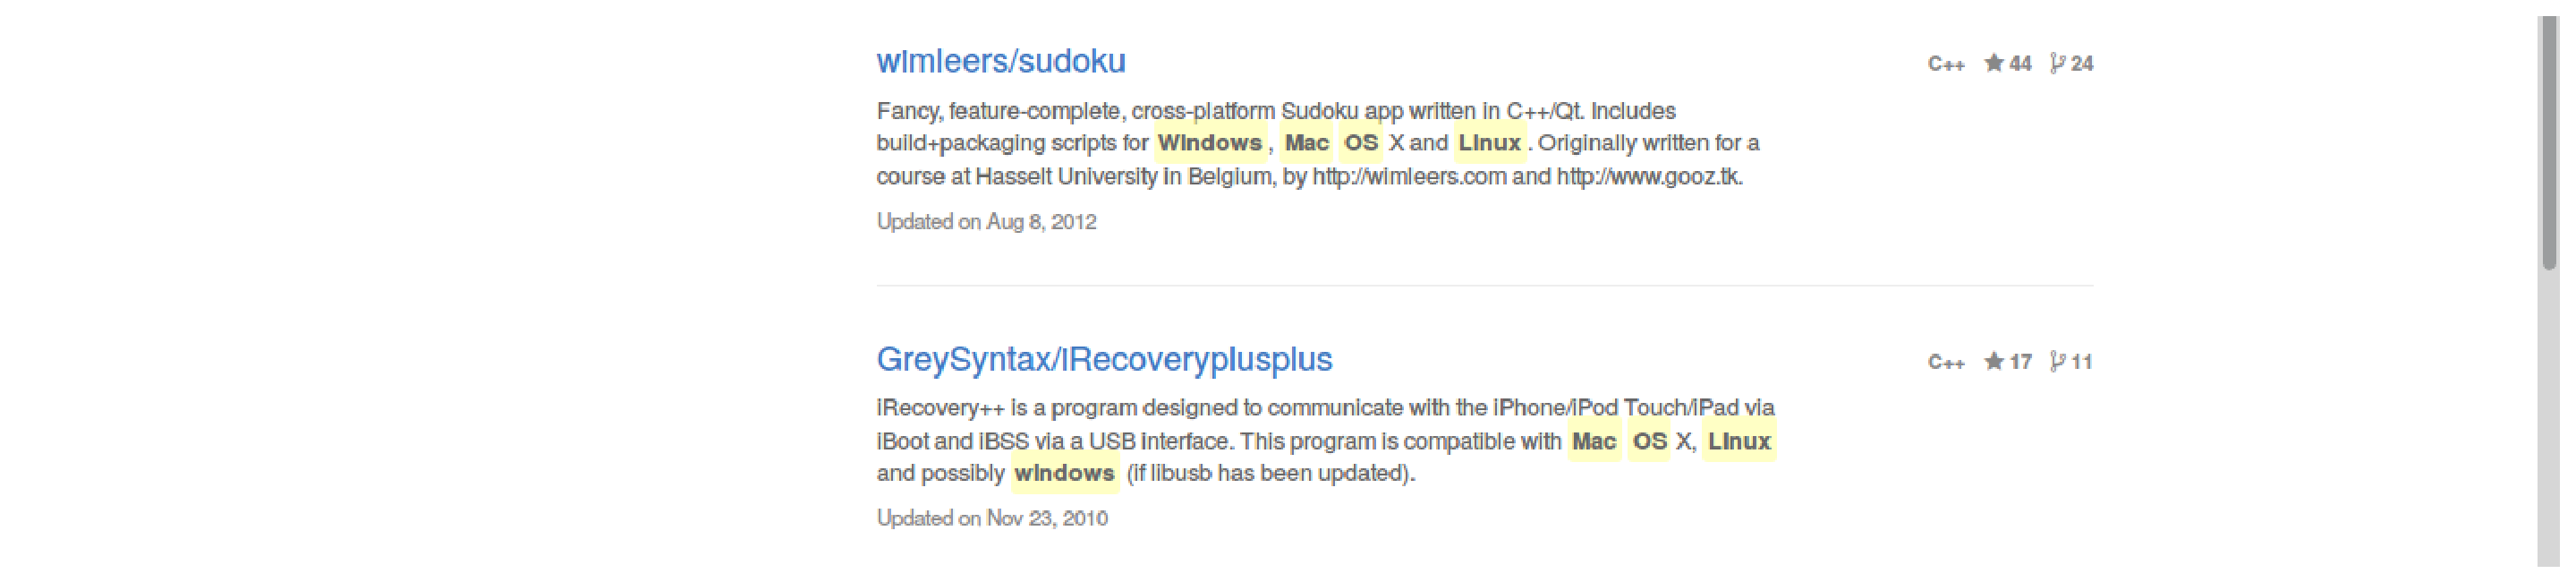
\includegraphics[scale=0.3]{figuras/github_search_2.eps}
    \caption{Pesquisa avançada Github parte 2}
    \label{pesquisa_github}
\end{figure}


\begin{table}[h]
\centering
\tiny
\begin{tabular}{llllll}
\textbf{Projeto} & \textbf{Linguagem} & \textbf{Estrelas} & \textbf{Forks} & \textbf{Porcentagem em C++} & \textbf{Gerador de Makefile}\\ \toprule
Aseprite & C++ & 437  & 77  & 62.1\% & CMake \\ \midrule 
Pencil & C++ &  161 & 22  & 54.6\%   & QMake \\ \midrule
Qcad & C++ & 110 & 51 & 80.8\%       & QMake \\ \midrule 
Sudoku & C++ &  44  & 24 & 94.9\%    & Qmake \\ \midrule
iRecoveryplusplus & C++ & 17 & 11 & 84.7\% & -  \\ \bottomrule
\end{tabular} 
\caption{Projetos Selecionados}
\tiny
\label{projetos_selecionados}
\end{table}


\subsection{Sobre os Projetos}

\begin{itemize}
    \item \textbf{Asepriter}
\footnote{\url{http://www.aseprite.org/}} é uma ferramenta para criação de sprites,
 compostas por camadas e quadros, suportadas em RGBA, paleta de 256 cores e escala de cinza.
 Permite visualizar a animação em tempo real e contém ferramentas para preencher contornos
 e polígonos. Esta ferramenta e open source e livre, e pode ser encontrada no \textit{github}
\footnote{\url{https://github.com/aseprite/aseprite}} ou no site da ferramenta
\footnote{\url{http://www.aseprite.org/}}.

    \begin{figure}[h]
        \centering
            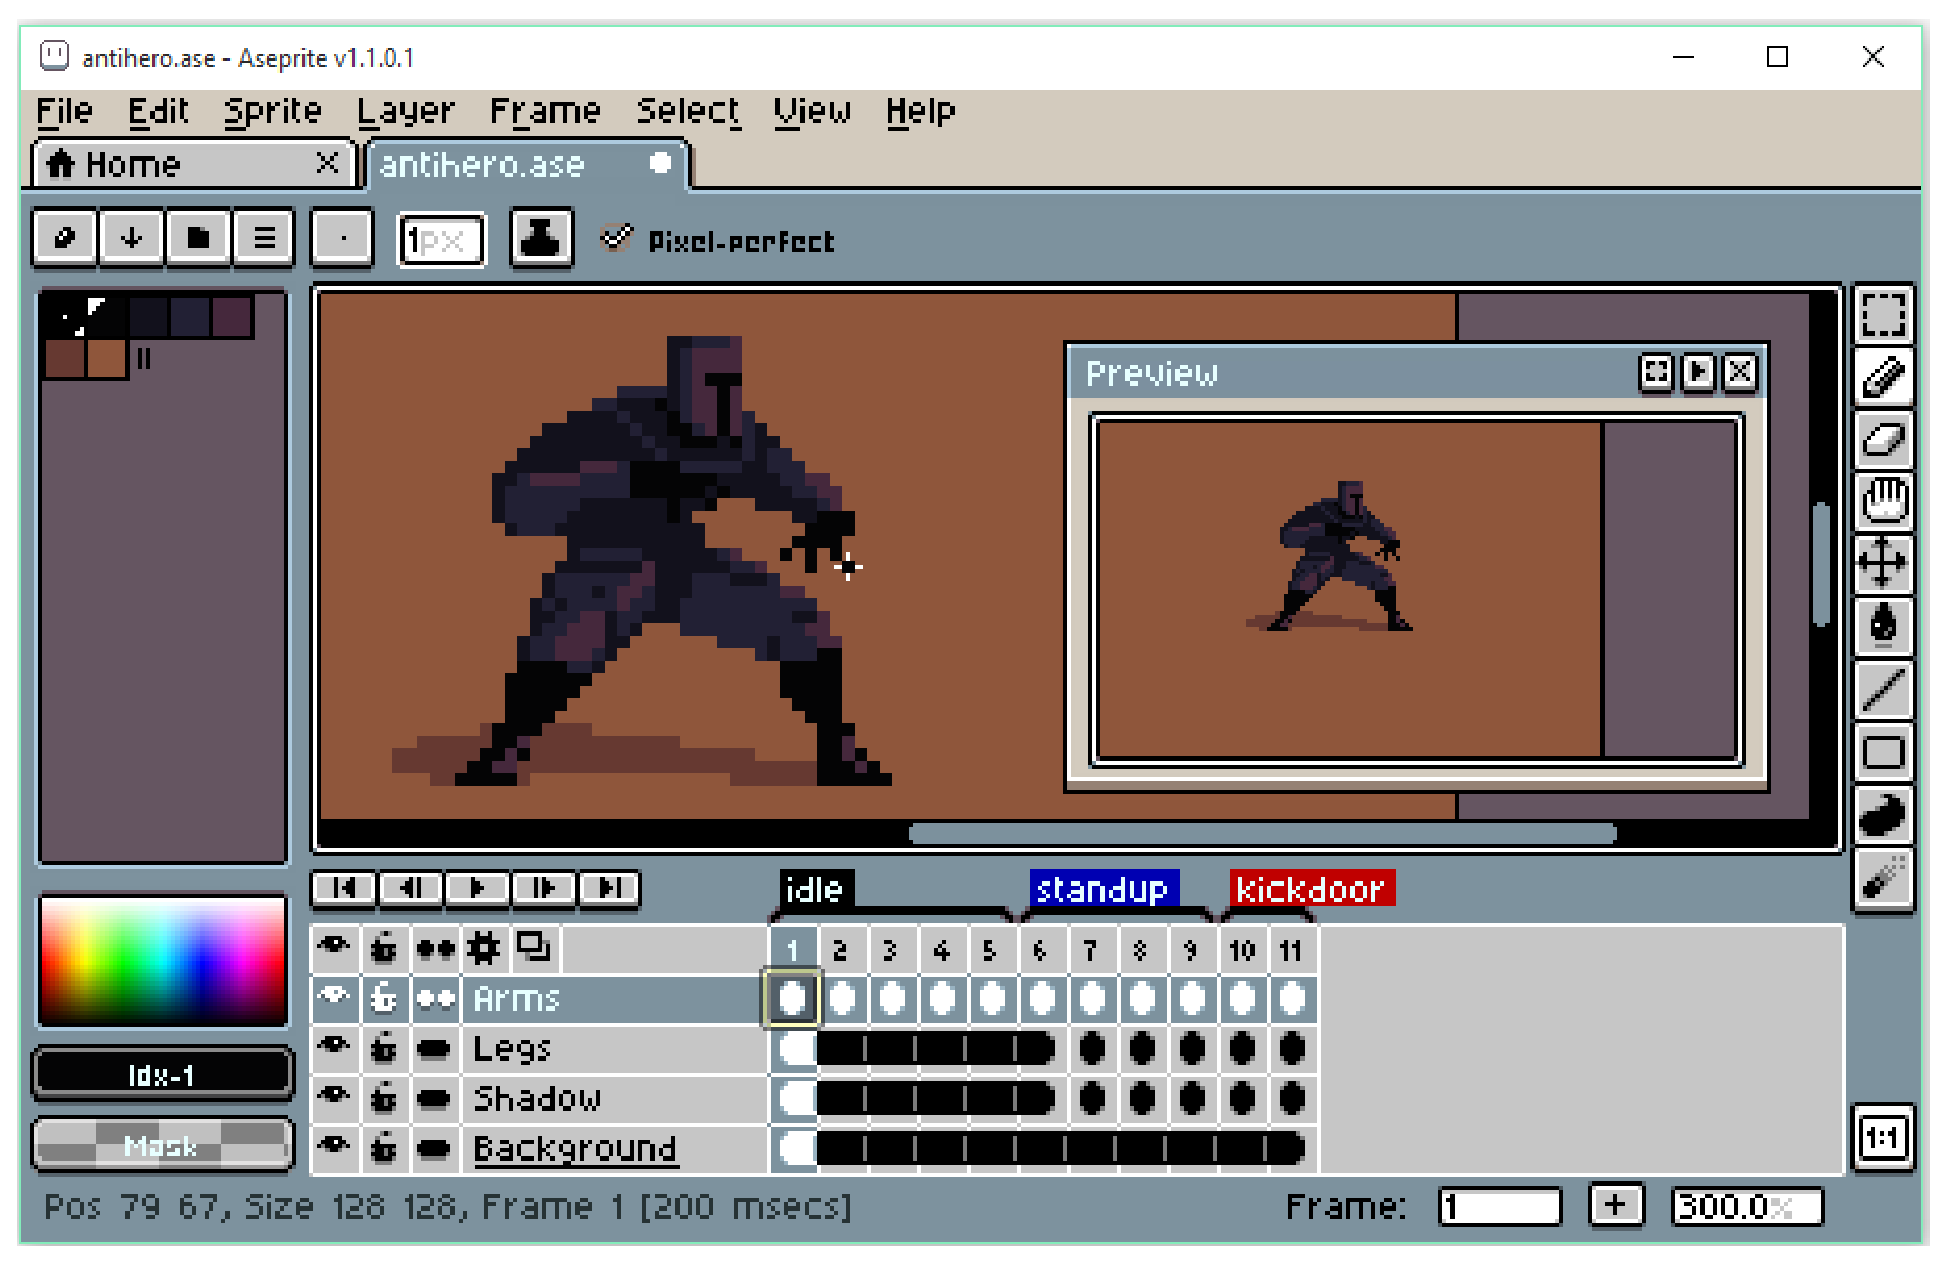
\includegraphics[scale=0.3]{figuras/aseprite.eps}
        \caption{Imagem da ferramenta Aseprite}
        \label{ferramenta_aseprite}
    \end{figure}

    \item \textbf{}
\footnote{\url{http://www.pencil2d.org/pencil2d/}} é uma ferramenta para
 desenho e animação desenhada a mão, e utilizando desenhos em formato bitmap ou gráfico vetoriais. 
Esta ferramenta é gratuita  e open source, podendo ser encontrada em no \textit{github}
\footnote{\url{https://github.com/pencil2d/pencil}} ou no site da ferramenta
\footnote{\url{http://www.pencil2d.org}}.

    \begin{figure}[h]
        \centering
            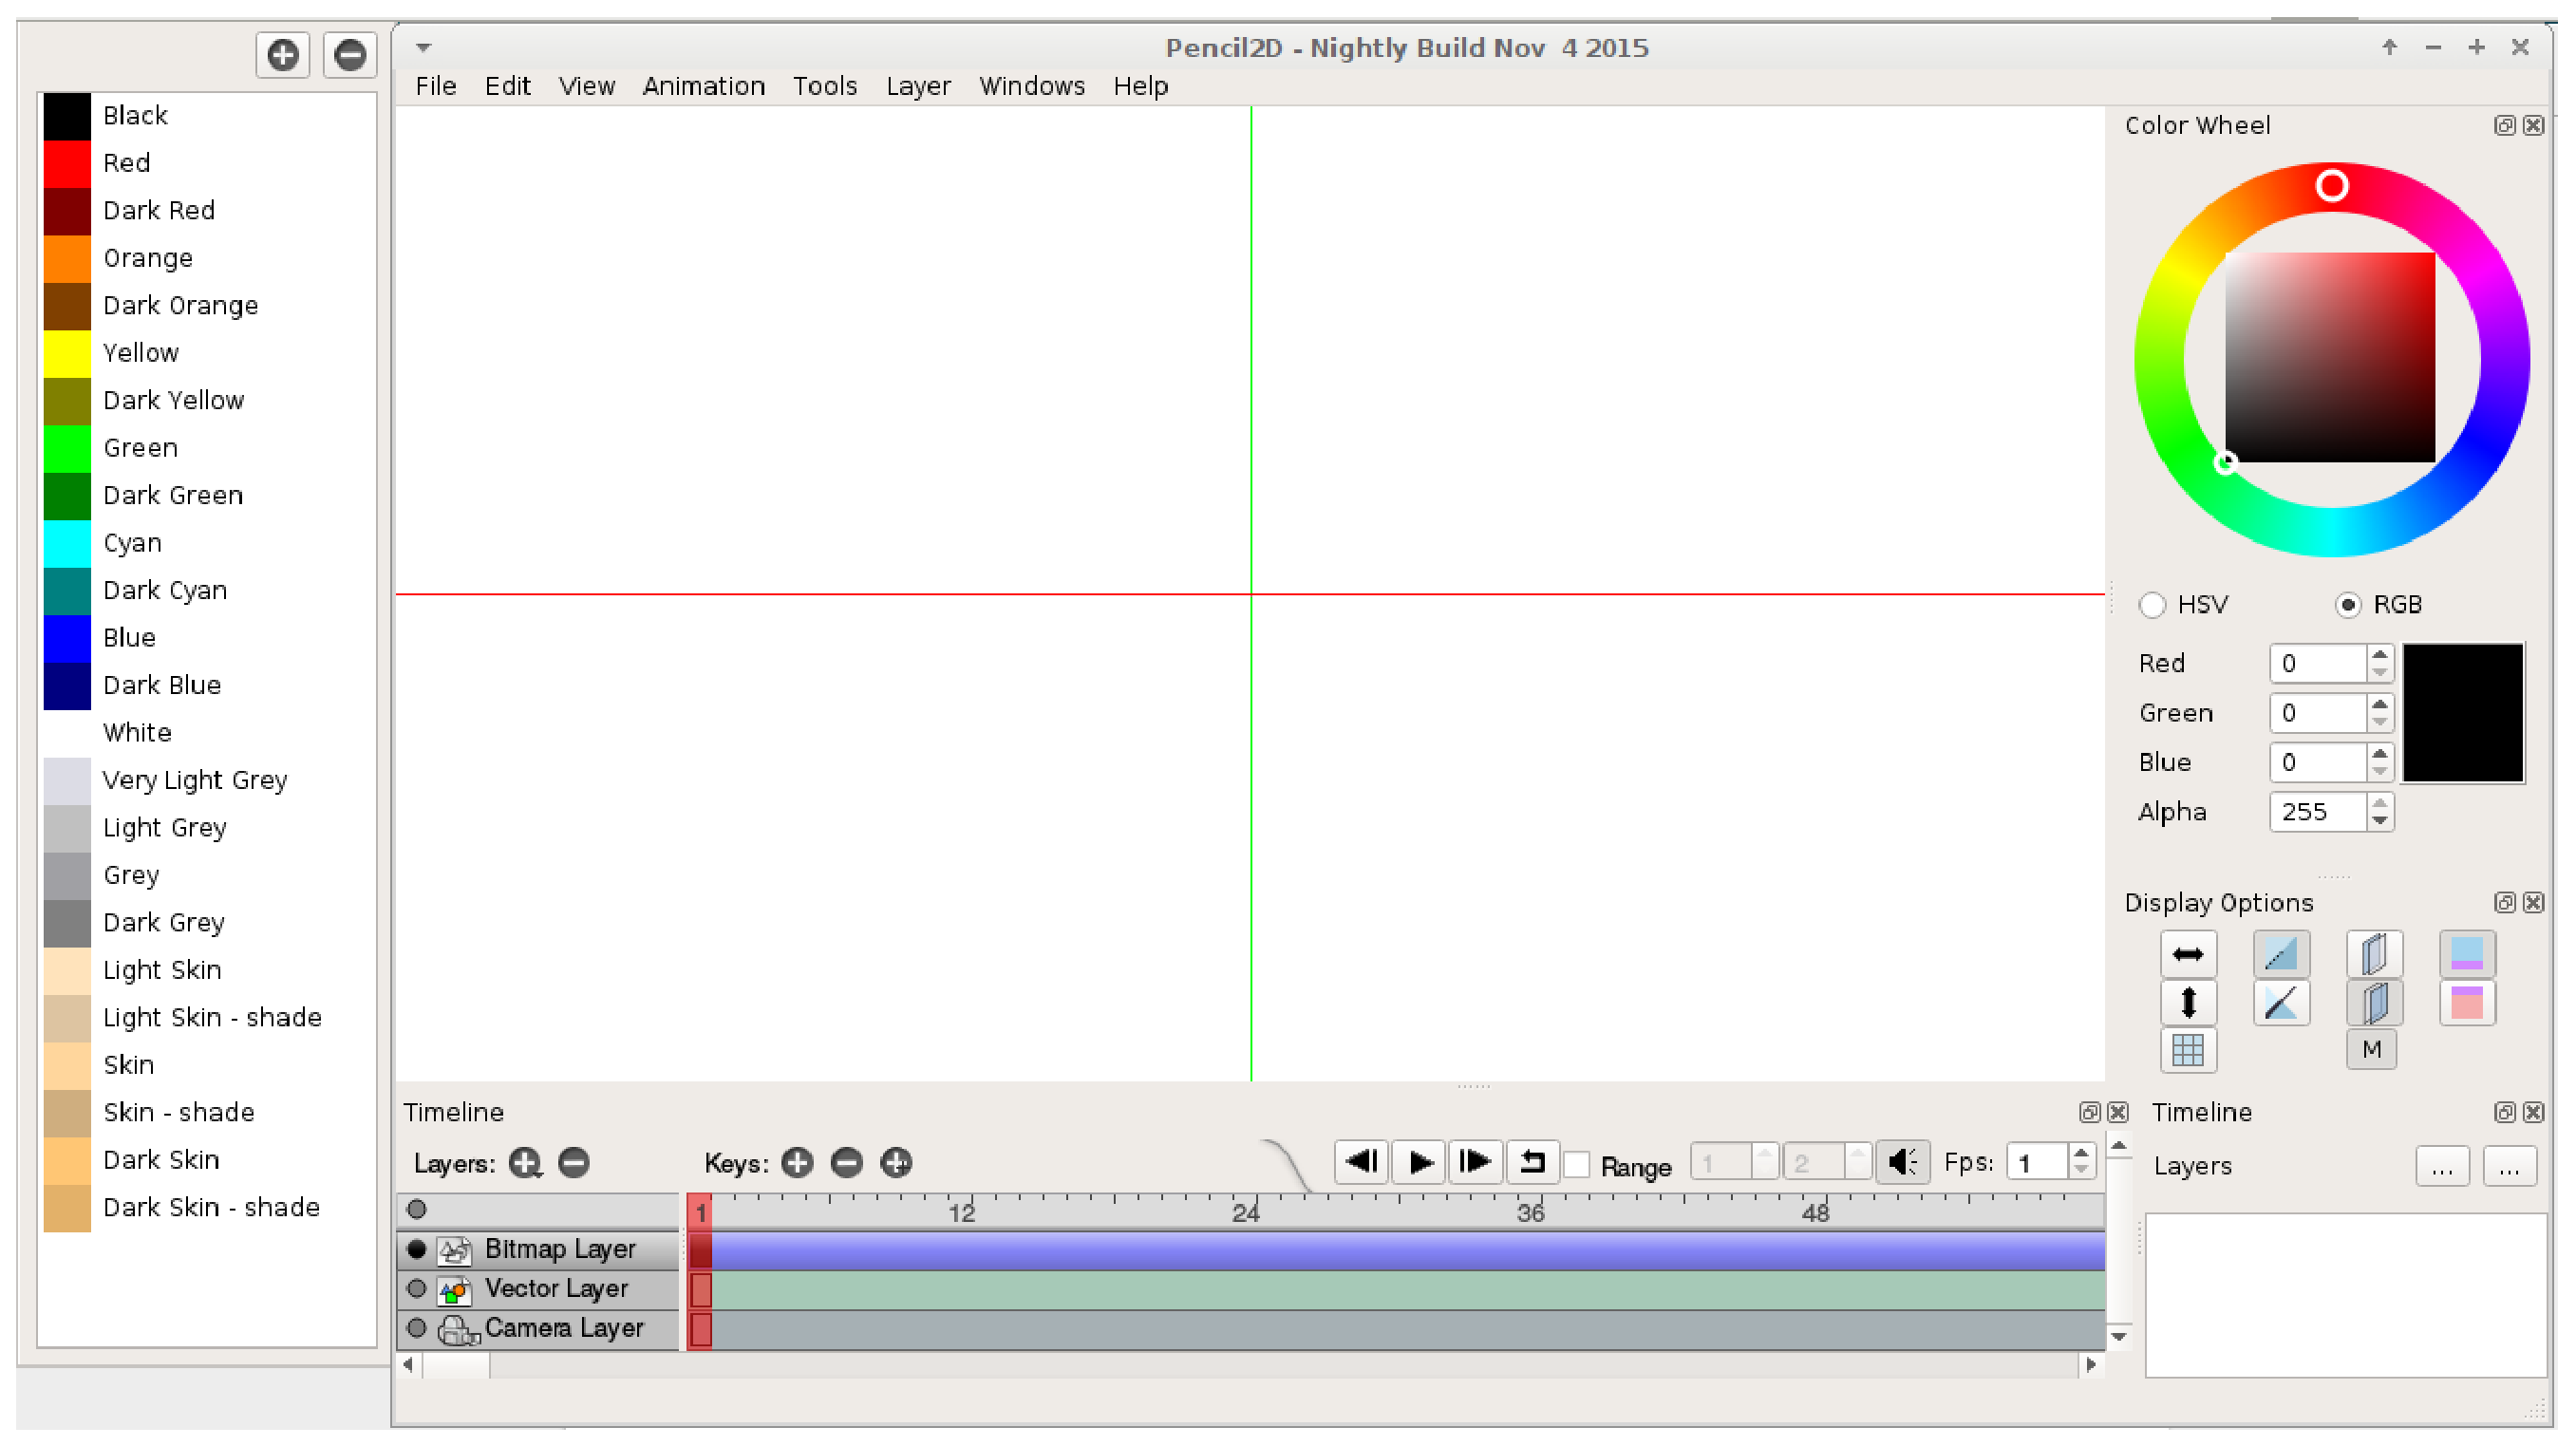
\includegraphics[scale=0.3]{figuras/pencil2D.eps}
        \caption{Imagem da ferramenta }
        \label{ferramenta_pencil2D}
    \end{figure}

    \item \textbf{Qcad}
\footnote{\url{http://www.qcad.org/en/}} é um software para desenho
 assistido por computador em duas dimensões, permitindo a criação de desenhos técnicos como
 planos para edifícios, interiores, peças mecânicas ou esquemas e diagramas. Esta ferramenta
 e open source  e gratuita e podendo ser encontrada no \textit{github}
\footnote{\url{https://github.com/qcad/qcad}} ou no site da ferramenta.
\footnote{\url{http://www.qcad.org/en/}}

    \begin{figure}[h]
        \centering
            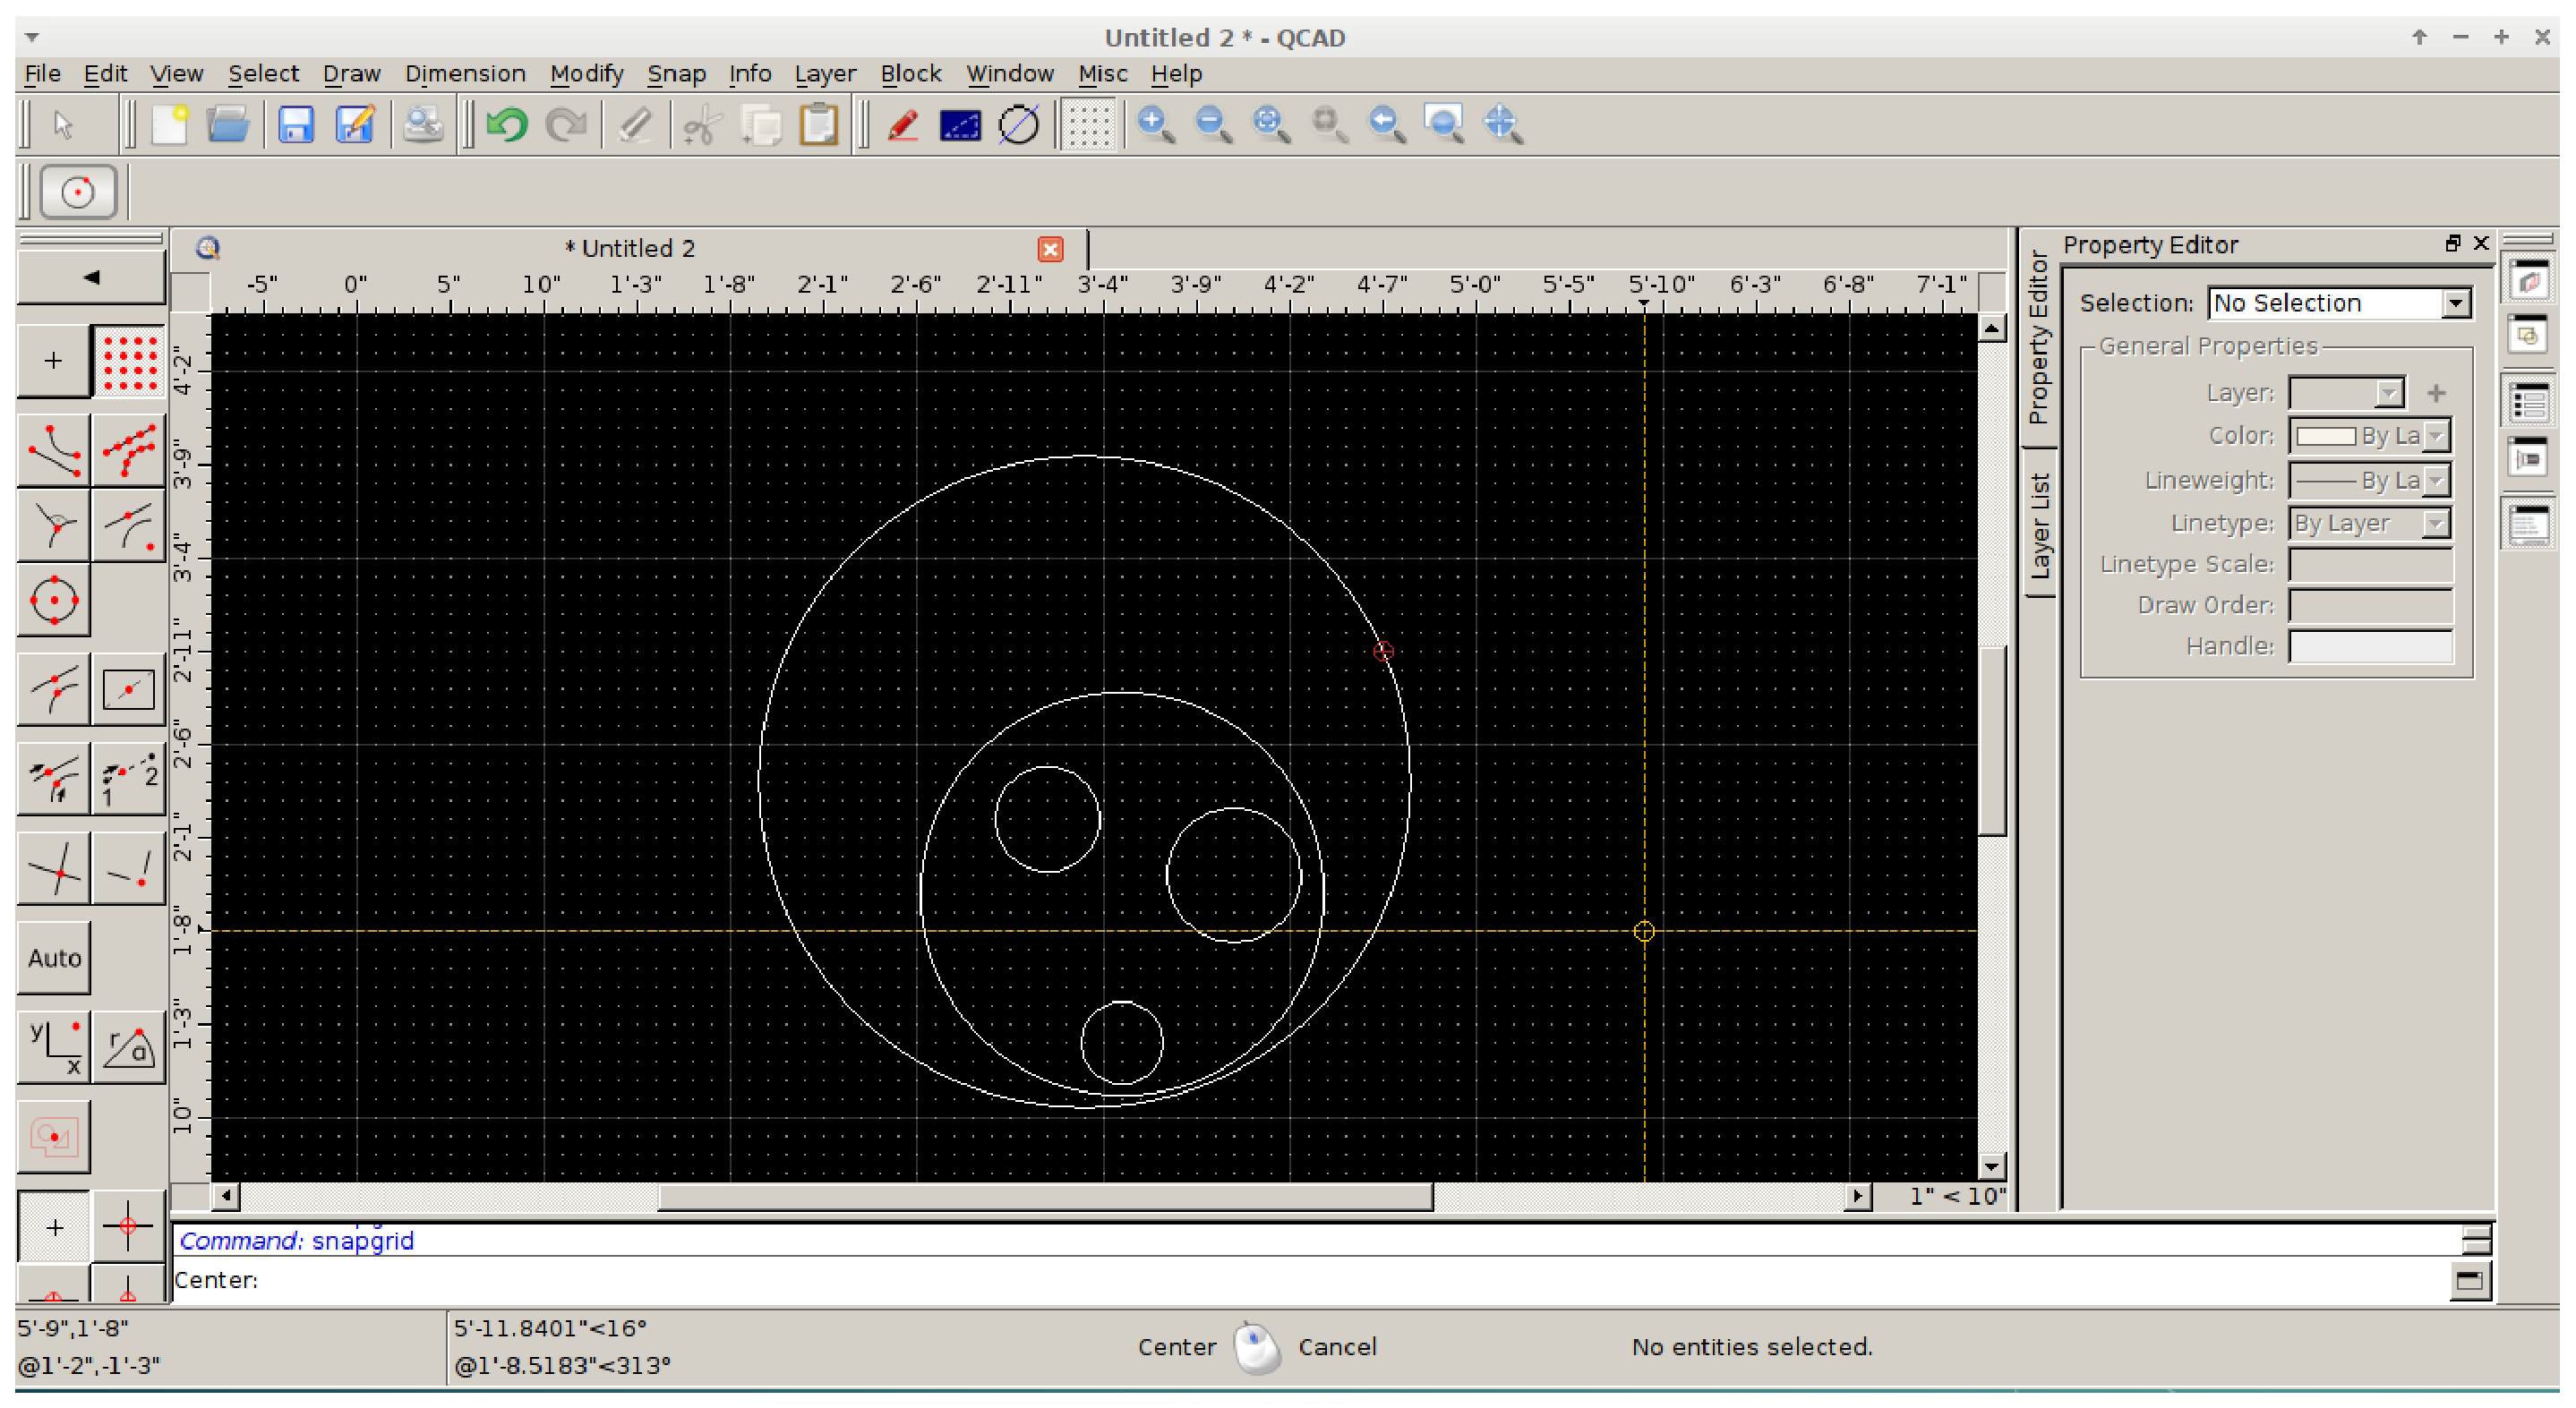
\includegraphics[scale=0.3]{figuras/qcad.eps}
        \caption{Imagem da ferramenta Qcad}
        \label{ferramenta_qcad}
    \end{figure}

    \item \textbf{Sudoku}
\footnote{\url{https://github.com/macartur-tcc/sudoku}} é um software que foi
 desenvolvido em um curso na universidade de Hasselt na Bélgica, esta foi escrita em c++ e utilizando Qt.
 Este é um software livre e liberado para domínio publico e pode ser encontrado apenas no \textit{github}
\footnote{\url{https://github.com/macartur-tcc/sudoku}}.

    \begin{figure}[h]
        \centering
            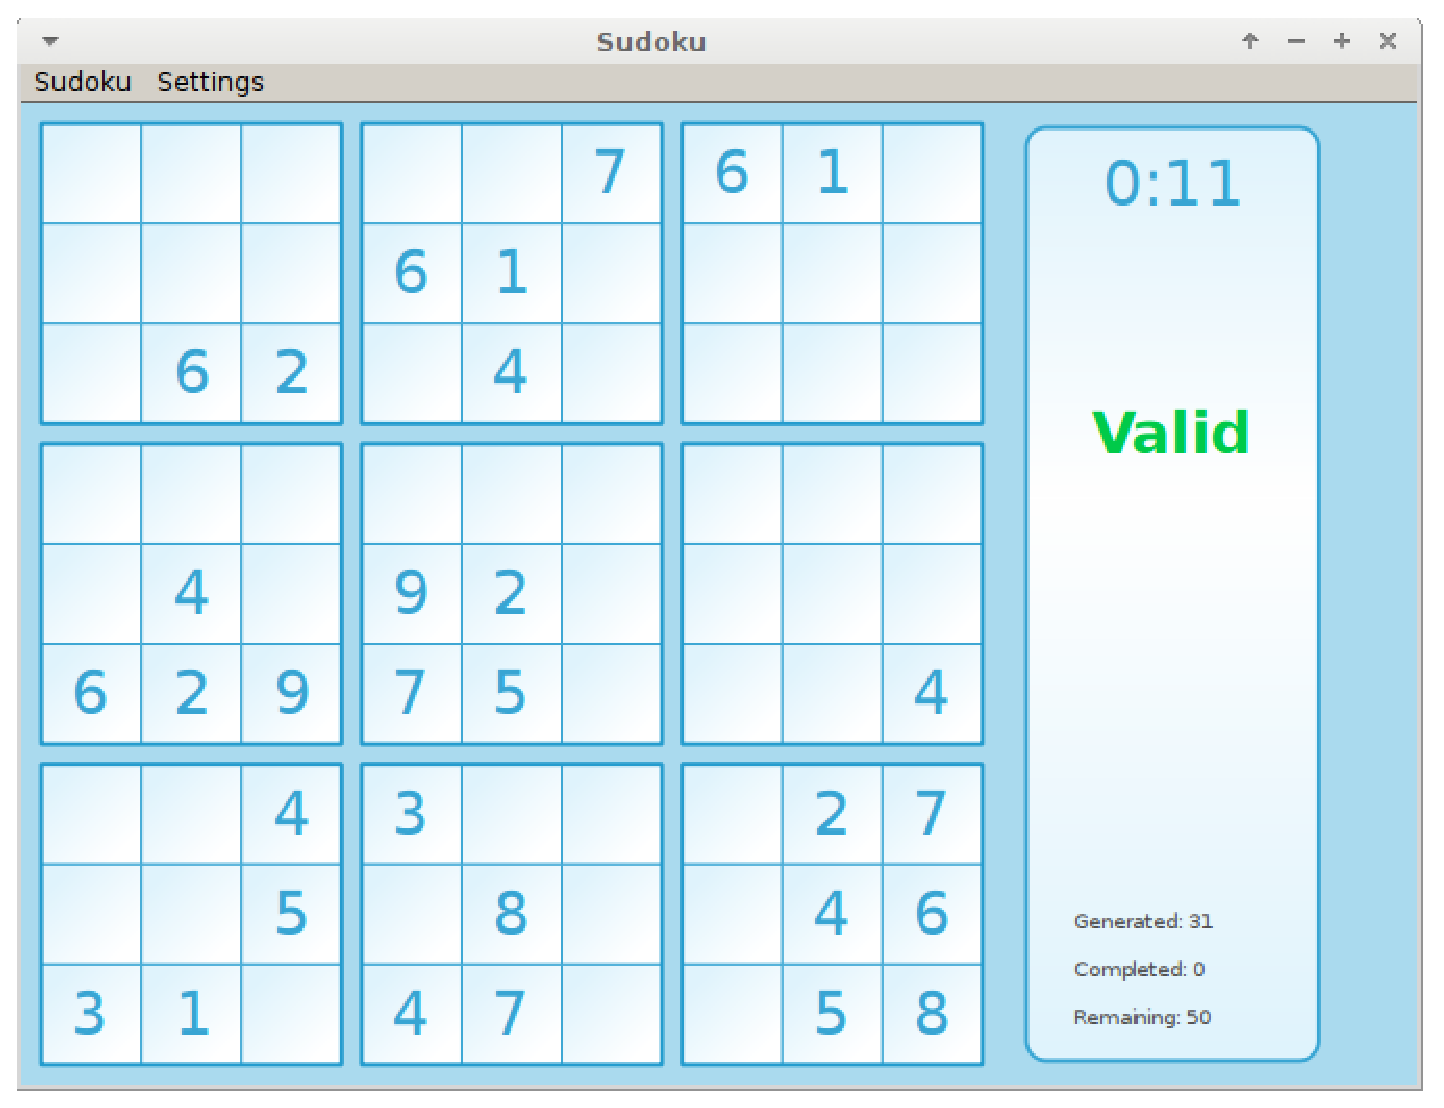
\includegraphics[scale=0.3]{figuras/sudoku.eps}
        \caption{Imagem da ferramenta Sudoku}
        \label{ferramenta_qcad}
    \end{figure}

    \item \textbf{iRecoveryplusplus}
\footnote{\url{https://github.com/GreySyntax/iRecoveryplusplus}} é um programa projetado para
 realizar comunicação de iPod, iPhone e iPad iBoot/iBSS  com interface USB. 
Este é um software livre e sobre a licença GPV v3 e pode ser encontrado no \textit{github}
\footnote{\url{https://github.com/GreySyntax/iRecoveryplusplus}} e é suportado em Linux, Mac OS e Windows.

\end{itemize}




\section{Ambiente}

\subsection{Ambiente Físico}

Para a realização dos estudos foi utilizado uma máquina com as
 especificações listada na tabela \ref{configuracoes_ambiente_fisico}

\begin{table}[h]
\centering
\begin{tabular}{lllll}
\textbf{Sistema Operacional} & \textit{Ubuntu} 14.04 \\ \toprule
\textbf{Kernel} & 3.19  \\ \midrule 
\textbf{Processador} & Intel i5 2.0Ghz \\ \midrule
\textbf{Memória Ram} & 4G  \\ \bottomrule 
\end{tabular} 
\caption{Configurações do Ambiente Físico}
\label{configuracoes_ambiente_fisico}
\end{table}


Nesta máquina foi instalado os programas:

\begin{itemize}
    \item \textbf{VirtualBox} - 4.0 : é uma ferramenta open source sobre a
 licença GPL v2 que permite a virtualização de máquinas.
    \item \textbf{Vagrant} - 1.7.4 : ferramenta de controle de
 máquina virtual possibilitando fácil acesso, criação, destruição, ligar e 
desligar máquinas virtuals.
    \item \textbf{Git} - 2.5.1 : ferramenta de controle de versão descentralizada
com o mesmo objetivo do \textit{SubVersion}(\textbf{SVN}).
\end{itemize}

\subsection{Ambiente Virtual}

\begin{itemize}

    \item \textbf{Linux}
        \subitem  O ambiente virtual Linux foi criado utilizando a box
 ubuntu/trusty64\footnote{\url{https://atlas.hashicorp.com/ubuntu/boxes/trusty64}},
 com a configuração do Vagrantfile no código \ref{vagrant_linux} e com especificações
 da máquina virtual mostradas na tabela \ref{especificacoes_linux}.
 Depois que construída a máquina virtual foram instalados os pacotes utilizando o
 gerenciador de pacotes apt, e estão listados na tabela \ref{pacotes_instalados_linux}.

Em ambiente linux o compilador padrão de C++ que vem instalado é o gcc/g++, este foi
 criado pela GNU e contém um conjunto de ferramentas para realizar, pré-processamento,
 compilação, montagem e link-edição. No front-end este compilador inclui as linguagens C,
 C++, Objective-C, Fortran, Java, Ada e Go, bem como bibliotecas
 (stdlibc++, libgcj, entre outras).


\begin{lstlisting}[language=ruby, caption={Vagrantfile com configurações da máquina virtual linux},
                  label=vagrant_linux]
    # Vagrantfile
    Vagrant.configure(2) do |config|
        config.vm.define 'linux' do |linux|
            linux.vm.box = "ubuntu/trusty64"
            linux.vm.network 'private_network', ip: "10.10.10.4"
            linux.vm.provider "virtualbox" do |vm| 
                vm.cpus = 2
                vm.memory = 2048
            end
        end              
    end
\end{lstlisting}

\begin{table}[h]
\centering
\begin{tabular}{ll}
\textbf{Sistema Operacional} & \textit{Ubuntu} 14.04 x86\_64 \\ \toprule
\textbf{Kernel} & 3.13.0-45-generic  \\ \midrule 
\textbf{Processador} & 2 processadores Virtuais \\ \midrule
\textbf{Memória Ram} & 2GB  \\ \bottomrule 
\end{tabular} 
\caption{Configurações do Ambiente Vitual Linux}
\label{especificacoes_linux}
\end{table}

\begin{table}[h]
\centering
\begin{tabular}{ll}
\textbf{Pacote} & \textbf{Versão} \\ \toprule
Qt5-default & 5.5.1 \\ \midrule 
Qt4-default & 4.8.7 \\ \midrule 
libusb-1.0-0/libusb-1.0-0-dev & 1.0.17-1ubuntu2 \\ \midrule 
libreadline6/libreadline6-dev & 6.3-4ubuntu2 amd6 \\ \midrule 
zlib1g/zlib1g-dev & 1.2.8.dfsg-1ubuntu1 amd6 \\ \midrule 
zlibc & 0.9k-4.1  \\ \midrule
g++/gcc  &  4:4.8.2-1ubuntu6 \\ \midrule 
git & 1.9.1-1 \\ \midrule 
cmake &   2.8.12.2  \\ \midrule 
ccache & 3.1.9  \\ \bottomrule 
\end{tabular} 
\caption{Pacotes instalados no Ambiente Virtual Linux}
\label{pacotes_instalados_linux}
\end{table}

    \item \textbf{Mac OS Yosemite}
        \subitem Para o ambiente Mac OS foi utilizada uma box com o sistema
 operacional na versão Yosemite 10.10.4
\footnote{\url{http://files.dryga.com/boxes/osx-yosemite-0.2.1.box}},
 com as configurações do Vagrantfile no código \ref{vagrant_mac_os_x} e com
 especificações da máquina virtual mostradas na tabela \ref{especificicacoes_mac_os_x}.
 Após a máquina criada foi necessário instalar os pacotes utilizando o gerenciador de
 pacotes brew, e foram listados os pacotes listados na tabela
\ref{pacotes_instalados_mac_os_x}.
Além dos listados foi necessário instalar o pacote "\textbf{MacOSX10.4.Universal.pkg}”
\footnote{\url{https://github.com/macartur-tcc/aseprite/blob/master/INSTALL.md}}
 disponibilizado pela Apple \footnote{\url{https://developer.apple.com/downloads/}}.

        \subitem Em um ambiente Mac OS o LLVM
\footnote{LLVM: infraestrutura de compilação utilizando o principio de modularização
 e reuso, propondo otimizar a compilação, execução e link-edição de programas
 escritos em linguagens variadas}é o back-end do compilador e como front-end
 padrão possui o clang/clang++, que foi projetado para ser 3 vezes mais rápido
 que o gcc/g++. As linguagens aceitas pelo clang são Objective-C, Fortran,
 Ada, Haskell, Java, Python, Ruby, ActionScript, GLSL, Julia, entre outras.


\begin{lstlisting}[language=ruby, caption={Vagrantfile com configurações da máquina virtual Mac OS Yosemite},
                  label=vagrant_mac_os_x]
    # Vagrantfile
    Vagrant.configure(2) do |config|
      config.vm.define 'mac_os_x' do |mac_os_x|
        mac_os_x.vm.box = "mac_os_x"
        mac_os_x.vm.network 'private_network', ip: "10.10.10.3"
        mac_os_x.vm.synced_folder "projetos", "/vagrant", type: "rsync"

        mac_os_x.vm.provider "virtualbox" do |vm|
          vm.gui = true
          vm.memory = 2024
        end
      end
    end

\end{lstlisting}

\begin{table}[h]
\centering
\begin{tabular}{ll}
\textbf{Sistema Operacional} & \textit{OS X Yosemite} x86\_64  \\ \toprule
\textbf{Kernel} & Darwin Kernel  14.4.0  \\ \midrule 
\textbf{Processador} & 2 processadores Virtuais \\ \midrule
\textbf{Memória Ram} & 2GB  \\ \bottomrule 
\end{tabular} 
\caption{Configurações do Ambiente Vitual Mac OS Yosemite}
\label{especificacoes_mac_os_x}
\end{table}


\begin{table}[h]
\centering
\begin{tabular}{ll}
\textbf{Pacote} & \textbf{Versão} \\ \toprule
qt5 & 5.5.1 \\ \midrule 
qt4 & 4.8.7 \\ \midrule 
libusb & 1.0.20 \\ \midrule 
readline & 6.3-8 \\ \midrule
zlib & 1.2.8 \\ \midrule
git & 1.9.1-1 \\ \midrule
cmake & 3.3.0  \\ \midrule
binutils & 2.25-4 \\ \midrule
ccache & 3.2.3 \\ \bottomrule
\end{tabular} 
\caption{Pacotes instalados no Ambiente Virtual Mac OS Yosemite}
\label{pacotes_instalados_mac_os_x}
\end{table}

    \item \textbf{Windows}
        \subitem Para o ambiente virtual Windows foi utilizado uma box com
 o sistema operacional Windows7\footnote{\url{https://vagrantcloud.com/datacastle/boxes/windows7}},
 com as configurações do Vagrantfile mostrada no código \ref{vagrant_windows},
 e com especificações da máquina virtual mostradas na tabela \ref{especificacoes_windows}.
 Para a utilização de um ambiente de desenvolvimento no windows é necessário a instalação
 do software \textit{cygwin}\footnote{\url{https://www.cygwin.com/}} que permite a instalação
o dos pacotes necessários para a criação do ambiente igual ao Unix.
 Utilizando o \textit{cygwin} é necessário instalar todos os pacotes para o sistema 
conseguir compilar programas em c++/c, para isto foram instalados os programas 
que se segue na tabela \ref{pacotes_instalados_windows}.

\begin{lstlisting}[language=ruby, caption={Vagrantfile com configurações da máquina virtual Windows 7},
                  label=vagrant_windows]
    #Vagrantfile
    Vagrant.configure(2) do |config|
      config.vm.define 'win7' do |win|
        win.vm.box = 'win7ie8'
        win.vm.network 'private_network', ip: '10.10.10.5'
        win.vm.provider 'virtualbox' do |vm|
              vm.cpus = 2
              vm.gui = true
              vm.memory = 1024
        end
      end
    end
\end{lstlisting}

\begin{table}[h]
\centering
\begin{tabular}{ll}
\textbf{Sistema Operacional} & \textit{Windows 7} x86\\ \toprule
\textbf{Kernel} & CYGWIN\_NT-6.1  \\ \midrule 
\textbf{Processador} & 2 processadores Virtuais \\ \midrule
\textbf{Memória Ram} & 2GB  \\ \bottomrule 
\end{tabular} 
\caption{Configurações do Ambiente Vitual Windows 7}
\label{especificacoes_windows}
\end{table}


\begin{table}[h]
\centering
\begin{tabular}{ll}
\textbf{Pacote} & \textbf{Versão} \\ \toprule
qt5-devel-tools  &  \\ 
qt5-translations & 5.5.1-1  \\ 
todos os pacotes que começam com este nome libQt5 & \\ \midrule

qt4-designer-plugin-webkit  & \\
qt4-devel-tools & 4.8.7-1 \\ 
qt4-qtconfig & \\ \midrule

libusb1.0 & 1.0.19-1 \\ \midrule


libreadline-devel & 6.3.8-1 \\ \midrule

zlib & 1.2.8 \\ \midrule
git & 2.5.3-1 \\ \midrule
ccache & 3.1.9-2 \\ \midrule
cmake & 3.3.2-1 \\ \midrule
cygwin-devel & 2.2.1 \\ \midrule
cygwin64-gcc-core & 4.9.2-1 \\ \midrule
gcc-core & \\ \midrule
gcc/g++ & 4.9.3-1 \\ 
make & 4.1-1 \\ \bottomrule
\end{tabular} 
\caption{Pacotes instalados no Ambiente Virtual Windows 7}
\label{pacotes_instalados_windows}
\end{table}

\end{itemize}



\section{Restrições de Compilação}

\subsection{Restrição Global}
    A utilização do linker gold não é possível compilar em todos os ambientes,
 pois é aplicada apenas a sistemas de arquivos binários ELF e nos ambientes
 Windows e Mac OS Yosemite os sistemas de arquivos são PE ou PE32+ e PEF 
respectivamente.

\subsection{Restrição Especifica}
    Em ambiente \textit{mingw} ou \textit{cygwin} não possui suporte
 a biblioteca glibc\footnote{
\url{https://www.gnu.org/software/gnulib/manual/html\_node/execinfo\_002eh.html}},
 isto fez com que o projeto Qcad que necessita do header exec\_info.h não possa ser compilado.

    Para alguns projetos foi necessário realizar modificações para a compilação
 dos mesmos nos diferentes sistemas operacionais,
estas alterações foram colocadas na branch master do repositório modificado,
utilizando um \textit{fork} do github
\footnote{\url{https://github.com/macartur-tcc/}} que contém todos os projetos.
 Esta restrição não impedindo a compilação dos projetos nos diferentes ambientes.

\section {Estudo de Caso}

\subsection{Aplicado no Ambiente}

Os casos de guardas de inclusão foram realizados utilizando script de benchmark,
 na qual os métodos detalhados na seção \ref{include_guards_section} foram
 aplicados a 10 mil arquivos com uma pequena quantidade de código
 \ref{codigo_27} e incluidos 3 vezes ao arquivo \textbf{main.cpp} utilizando
 \ref{codigo_28}. Cada um destes foram aplicados aos diferentes ambientes de
 desenvolvimento.

\begin{lstlisting}[language=C++,caption={Template de arquivo .hpp utilizado no benchmark},
                                                   label=codigo_27]

  // <NUMERO>.hpp

  const int int<NUMERO> = <NUMERO>;

\end{lstlisting}

\begin{lstlisting}[language=C++,caption={Template de arquivo main.cpp utilizado no benchmark},
                                                          label=codigo_28]

    // main.cpp

    /* headers a serem incluidos   */

    ...

    int main(){return 0;}
\end{lstlisting}

Os scripts abordam os métodos:

\begin{itemize}
	\item guarda de Inclusão Externa;
	\item guarda de Inclusão Interna;
	\item \textit{pragma once};
	\item guarda de Inclusão Interna primeiro que \textit{pragma once};
	\item \textit{pragma once} primeiro que  Guarda de Inclusão Interna;
	\item guarda de Inclusão Externa + \textit{pragma once};
	\item redundância de Guarda de Inclusão.
\end{itemize}

\subsection{Aplicado no Projeto}

Antes da realização do estudo de caso foi necessário identificar quais
 as técnicas que poderiam ser aplicadas em cada um dos projetos.
 As tabelas \ref{tecnicas_que_podem_ser_aplicadas_codigo}, \ref{tecnicas_que_podem_ser_aplicadas_flag} e 
\ref{tecnicas_que_podem_ser_aplicadas_ferramenta} mostram esta analise.


\begin{table}[h]
\centering
\begin{tabular}{llll}
\textbf{Projeto} & \textbf{pragma once} & \textbf{Forward Declaration} & \textbf{Pimpl Idiom}  \\ \toprule 
iRecoveryplusplus & SIM & SIM & SIM  \\ 
Sudoku &  SIM & SIM & SIM  \\ 
Pencil & SIM & NÃO &  SIM \\ 
Aseprite &  SIM & NÃO & NÃO  \\ 
Qcad &  SIM & NÃO & NÃO  \\ \bottomrule
\end{tabular} 
\caption{Técnicas que podem ser aplicadas ao código}
\label{tecnicas_que_podem_ser_aplicadas_codigo}
\end{table}

\begin{table}[h]
\centering
\begin{tabular}{lll}
\textbf{Projeto} & \textbf{Makafile} &  \textbf{Otimização de Baixo Nível} \\ \toprule
iRecoveryplusplus & SIM & SIM\\ 
Sudoku &  SIM & SIM  \\ 
Pencil &  SIM & SIM  \\ 
Aseprite & SIM & SIM  \\ 
Qcad &   SIM & SIM\\ \bottomrule
\end{tabular} 
\caption{\textit{Flags} que podem ser utilizadas}
\label{tecnicas_que_podem_ser_aplicadas_flag}
\end{table}

\begin{table}[h]
\centering
\begin{tabular}{lll}
\textbf{Projeto} &  \textbf{Ccache} & \textbf{Gold} \\ \toprule 
iRecoveryplusplus &  SIM & SIM \\ 
Sudoku            &  SIM & SIM \\ 
Pencil            &  SIM & SIM \\ 
Aseprite          &  SIM & SIM \\ 
Qcad              &  SIM & SIM \\ \bottomrule
\end{tabular} 
\caption{Ferramentas que podem ser utilizadas}
\label{tecnicas_que_podem_ser_aplicadas_ferramenta}
\end{table}


\subsubsection{Alteração de Código}

 Para as alterações de código, cada caso foi criado
 uma branch com suas modificações e estas estão no repositório
 destinado ao TCC\footnote{\url{https://github.com/macartur-tcc/}}.

    \begin{enumerate}
        \item Pragma Once
        \subitem Neste estudo de caso os arquivos de header foram alterados
 com a inclusão da diretiva “\#pragma once” no inicio de cada arquivo.
 No projeto aseprite está sendo removido a diretiva, pois todos os arquivos já possuem.
Estas alterações estão na branch “\textit{pragma\_once}” dos projetos que foi possível aplicar.
        \item Forward Declaration
        \subitem Neste estudo de caso os headers foram alterados para reduzir
 a quantidade de headers de todos os cabeçalhos e das implementação.
 Para isso foram removidos headers redundantes e que referenciava
 ponteiros e referências de endereço.
Estas alterações estão na branch "\textit{forward\_declaration}" dos projetos que foi possível aplicar.
        \item Técnicas de Pimpl Idiom
        \subitem Neste estudo de caso atributos e métodos privados foram removidos do cabeçalho
 e incluídos nos arquivos de implementação, como no exemplo de código \ref{exemplo_implementacao_pimpl}
 da seção \ref{Pimpl_Idiom}
 que demostra como aplicar a técnica.
Estas alterações estão na branch "\textit{pimpl}" dos projetos que foi possível aplicar.
    \end{enumerate}

\subsubsection{Alteração de flags de Compilação}

        \begin{enumerate}
            \item makefile
                \subitem Neste estudo de casos no momento da utilização do makefile
 será utilizado as flags: -j2,-j4,-j6,-j8 e -j10. Com este resultará na relação entre
a compilação e a quantidade de \textit{jobs}(\textit{threads}).
            \item Otimização de Baixo Nível
                \subitem Neste estudo de caso todos os arquivos Makefile serão
 alterados para receber a flags: -O, -O0, -O2, -Ofast, -O3, -Os,-Og.
 Com estes resultados será possível verificar a relação do tempo gasto com
 o tempo de otimização do compilador.
        \end{enumerate}

\subsubsection{Ferramentas Auxiliares}

        \begin{enumerate}
               \item CCache
                    \subitem Neste estudo de caso em cada projeto será adicionado
 a palavra ccache antes de cada linha de compilação. Será utilizado as
 configurações padrão do ccache, e antes de cada compilação para ter certeza
 que toda a cache será removida utilizará o comando ccache -C e ccache -c.
                \item Gold
                    \subitem Neste estudo de caso será ativado o ld.gold
 utilizando a flag:-Wl,-fuse-ld=gold como mostrado na seção \ref{Gold}. Assim  a
 compilação irá deixar de utilizar o linker padrão e utilizará o linker
 otimizado para sistema ELF.
        \end{enumerate}

\subsubsection{Passos de Compilação dos projetos}

\begin{itemize}
       \item {iRecoveryplusplus}
        \subitem Para compilar o projeto iRecoveryplusplus é necessário
 realizar o clone do projeto no github, e compilar utilizando os comandos no Código 
\ref{clonando_irecoveryplusplus}.


\begin{lstlisting}[language=bash, caption={Clonado e compilando o projeto iRecoveryplusplus},
                  label=clonando_irecoveryplusplus]

    # clonando o projeto
    $ git clone https://github.com/macartur-tcc/iRecoveryplusplus.git 
    $ cd iRecoveryplusplus

    # compilando no Linux, Mac OS Yosemite ou Windows 7
    $ make linux 
    
    # compilar utilizando o linker gold no Linux
    $ make linux  CC="gcc -Wl,-fuse-ld=gold" CXX="g++ -Wl,-fuse-ld=gold"

    # compilar utilizando a ferramenta ccache
    $ make linux CC="ccache gcc" CXX="ccache g++"

    # removendo arquivos binarios gerados
    rm bin/*
\end{lstlisting}

    \item \textbf{Sudoku}
    \subitem Para compilar o projeto Sudoku é necessário realizar o clone do projeto
no github utilizando os comandos no Cógido \ref{clonando_sudoku}.
\footnote{Neste projeto e necessário remover a flag -archi386 do arquivo Makefile gerado na raiz, pois em sistemas Mac OS esta flag causa erro.}

\begin{lstlisting}[language=bash, caption={Clonado e compilando o Projeto Sudoku},
                  label=clonando_sudoku]

    # clonando projeto do github 
    $ git clone https://github.com/macartur-tcc/sudoku.git 
    $ cd sudoku/src

    # gerando makefile
    $ qmake Sudoku_release.pro

    # compilando no Linux, Mac OS ou Windows 7
    $ make

    # compilar no Linux utiizando o linker gold
    $ make  CC="gcc -Wl,-fuse-ld=gold" CXX="g++ -Wl,-fuse-ld=gold"

    # compilando utilizando a ferramenta ccache
    $ make CC="ccache gcc" CXX="ccache g++"

    # remover arquivos binarios gerados
    $ make clean
    
\end{lstlisting}

    \item \textbf{Pencil}
    \subitem Para compilar o projeto Pencil é necessário realizar
 o clone do projeto no github e executar os comandos mostrados no
 Código \ref{clonando_pencil} 

\begin{lstlisting}[language=bash, caption={Clonado Projeto Pencil},
                  label=clonando_pencil]
    #clonando o projeto do github
    $ git clone https://github.com/macartur-tcc/pencil.git
    $ cd pencil

    # gerando makefile para ambiente Linux e Windows 7
    $ qmake -r

    # gerando makefile para ambiente Mac OS Yosemite
    $ qmake -r RESOURCES=./pencil.qrc  
    
    # compilando 
    $ make

    # compilando utilizando a ferramenta ccache
    $ make CC="ccache gcc" CXX="ccache g++"

    # compilando utilizando gold
    make CC="gcc -Wl,-fuse-ld=gold" CXX="g++ -Wl,-fuse-ld=gold"

    # removendo arquivos binarios gerados
    $ make clean

\end{lstlisting}

    \item \textbf{Aseprite}
    \subitem Para compilar o projeto Aseprite é necessário fazer o clone do projeto,
 gerar os arquivos makefile seguindo os comandos no Código \ref{clonando_aseprite}.

\begin{lstlisting}[language=bash, caption={Clonado Projeto Aseprite e criando diretório de Compilação},
                  label=clonando_aseprite]
    # clonado projeto do github
    $ git clone https://github.com/macartur-tcc/aseprite.git
    $ cd aseprite

    # criando diretorio para compilar o projeto
    $ mkdir build
    $ cd build

    # gerando makefile do projeto no Linux e Windows 7
    $ cmake -G .. "Unix Makefiles"

    # gerando makefile no Mac OS Yosemite
    $ cmake -G ... "Unix Makefiles" -DCMAKE_OSX_ARCHITECTURES:STRING=i386  -DCMAKE_OSX_DEPLOYMENT_TARGET:STRING=10.4  -DCMAKE_OSX_SYSROOT:STRING=/SDKs/MacOSX10.4u.sdk
    
    # compilando o projeto com ccache no Linux Windows 7
    $ cmake -G .. "Unix Makefiles"  -DCMAKE_CXX_COMPILER="ccache"  -DCMAKE_CXX_COMPILER_ARG1="g++" -DCMAKE_C_COMPILER="ccache" -DCMAKE_C_COMPILER_ARG1="gcc"

    # compilando projeto com ccache no Mac OS Yosemite
    $ cmake -G .. "Unix Makefiles"  -DCMAKE_CXX_COMPILER="ccache"  -DCMAKE_CXX_COMPILER_ARG1="g++" -DCMAKE_C_COMPILER="ccache" -DCMAKE_C_COMPILER_ARG1="gcc"  -DCMAKE_OSX_ARCHITECTURES:STRING=i386  -DCMAKE_OSX_DEPLOYMENT_TARGET:STRING=10.4  -DCMAKE_OSX_SYSROOT:STRING=/SDKs/MacOSX10.4u.sdk

    # compilando com o linker gold no Linux
    $ CC="gcc  -Wl,-fuse-ld=gold" CXX="g++ -Wl,-fuse-ld=gold" cmake .. -G "Unix Makefiles"

    # removendo arquivos binarios
    $ make clean

\end{lstlisting}


    \item \textbf{Qcad}
    \subitem Para compilar o projeto Qcad é necessário clonar o
 projeto no github, gerar os arquivos makefile e compilar
 utilizando os comandos descritos no Código \ref{clonando_qcad}.

\begin{lstlisting}[language=bash, caption={Clonado Projeto Qcad},
                  label=clonando_qcad]

    #clonando projeto do github
    $ git clone https://github.com/macartur-tcc/qcad.git
    $ cd qcad

    # compilando no Linux e Windows 7
    $ qmake -r
    
    # compilando no Mac OS Yosemite
    qmake -spec macx-g++ -r

    # compilando no Linux, Windows7 e Mac OS Yosemite
    $ make

    # compilando com a ferramenta ccache
    $ make CC="ccache gcc" CXX="ccache g++"

    # compilando com o linker gold
    $ make  CC="gcc -Wl,-fuse-ld=gold" CXX="g++ -Wl,-fuse-ld=gold"

    # removendo arquivos binarios gerados
    $ make clean

\end{lstlisting}
\end{itemize}


\section{Montagem de Scripts}


Os scripts foram elaborados utilizando a linguagem de programação python,
 e estão sendo armazenados no github
\footnote{\url{https://github.com/macartur-tcc/tcc_scripts}}.


\subsection{Aplicado ao Ambiente}\label{Amplicação ao Ambiente}

Para o estudo aplicado ao ambiente foi criado um script de benchmark utilizando
 a linguagem python, e foi detalhado no apêndice na seção Benchmark \ref{script_bench_mark}.

A Tabela \ref{tab:modelo_guards} representa o modelo utilizado na coleta dos dados,
 contendo Guarda de Inclusão Externa(GIE), Guarda de Inclusão Interna(GII),
 Pragma Once(PO), Guarda de Inclusão Interna Primeiro que Pragma Once(GIIPPO),
 Pragma Once Primeiro que Guarda de Inclusão Interna (POPGII),
 Guarda de Inclusão Externa e Pragma Once (GIEPPO) e
 Redundância de Guarda de Inclusão(RGI).

\begin{table}[!ht]
\centering
\caption{Template de amostra de Guardas de Inclusão}
\label{tab:modelo_guards}
\begin{tiny}
\begin{tabular}{lp{1cm}p{1cm}p{1cm}p{1cm}p{1cm}p{1cm}p{1cm}p{1cm}}

\textbf{Tipo} & \multicolumn{7}{l}{Utilização de Guarda de Inclusão} \\
\textbf{Medida} & \multicolumn{7}{l}{Tempos em segundos } \\
\textbf{Amostras} & \textbf{GIE} & \textbf{GII} & \textbf{PO} & 
\textbf{GIIPPO} & \textbf{POPGII} & \textbf{GIEPPO} & \textbf{RGI} \\ \toprule
 1  &  &  &   &   &   &   &  \\ 
 2  &  &  &   &   &   &   &  \\ 
 3  &  &  &   &   &   &   &  \\ 
 4  &  &  &   &   &   &   &  \\ 
 5  &  &  &   &   &   &   &  \\ 
 6  &  &  &   &   &   &   &  \\ 
 7  &  &  &   &   &   &   &  \\ 
 8  &  &  &   &   &   &   &  \\ 
 9  &  &  &   &   &   &   &  \\ 
 10 &  &  &   &   &   &   &  \\ \bottomrule
 Média: & & & & &   &   &    \\ 
\end{tabular}
\end{tiny}
\end{table}


\subsection{Aplicado a Projeto}

Para realizar as compilações dos projetos foi criado um script de recompilação que
 segue no código \ref{script_recompilacoes}, com este é possível alterar entre
 branch para compilar as alterações de código dos projetos,
 executar comandos antes e depois de cada compilação.
 Para receber todos estes comandos foi necessário a leitura de um arquivo de
 configuração de cada projeto contendo a localização do projeto,
 localização do makefile, comandos que serão executados antes e depois
 da compilação.
 Este arquivo foi escrito em yaml e seguindo o template do código
 \ref{template_para_script_recompilacoes}.
Para a contagem do tempo de compilação foi utilizado o módulo datetime do python,
 realizando a diferença do tempo inicial e final do tempo de compilação.

Após a execução do script será preenchida as tabelas abaixo, e gerado gráficos para melhor
analisar os resultados. 


\begin{table}[!ht]
\centering
\caption{Modelo Alteração de Código}
\label{tab:modelo_alteracao_de_codigo}
\begin{tabular}{lllll}
\textbf{<Nome do Projeto>} & \textbf{master} & \textbf{pragma once} & \textbf{forward declaration} & \textbf{private implementation}   \\ \toprule
1                             &      &     &     &        \\ 
2                             &      &     &     &        \\ 
3                             &      &     &     &        \\ 
4                             &      &     &     &        \\ 
5                             &      &     &     &        \\ 
6                             &      &     &     &        \\ 
7                             &      &     &     &        \\ 
8                             &      &     &     &        \\ 
9                             &      &     &     &        \\ 
10                            &      &     &     &        \\ \bottomrule
Média                         &      &     &     &        \\ 
\end{tabular}
\end{table}


\begin{table}[!ht]
\centering
\caption{Modelo Flags de Otimização da Compilação}
\label{tab:modelo_otimizacao_compilacao}
\begin{tabular}{llllllll}
\textbf{<Nome do Projeto>} & \textbf{-O} & \textbf{-O0} & \textbf{-O2} & \textbf{-O3} & \textbf{-Os} & \textbf{-Ofast} & \textbf{-Og} \\ \toprule
1                          &             &              &              &              &              &                 &        \\ 
2                          &             &              &              &              &              &                 &        \\ 
3                          &             &              &              &              &              &                 &        \\ 
4                          &             &              &              &              &              &                 &        \\ 
5                          &             &              &              &              &              &                 &        \\ 
6                          &             &              &              &              &              &                 &        \\ 
7                          &             &              &              &              &              &                 &        \\ 
8                          &             &              &              &              &              &                 &        \\ 
9                          &             &              &              &              &              &                 &        \\ 
10                         &             &              &              &              &              &                 &        \\ \bottomrule
Média                      &             &              &              &              &              &                 &        \\ 
\end{tabular}
\end{table}

\begin{table}[!ht]
\centering
\caption{Modelo Flags de Processamento Paralelo}
\label{tab:modelo_flag_processamento_paralelo}
\begin{tabular}{llllll}
\textbf{<Nome do Projeto>} & \textbf{-j 2} & \textbf{-j 4} & \textbf{-j 6} & \textbf{-j 8} & \textbf{-j10}  \\ \toprule
1                                    &    &     &     &     &        \\ 
2                                    &    &     &     &     &        \\ 
3                                    &    &     &     &     &        \\ 
4                                    &    &     &     &     &        \\ 
5                                    &    &     &     &     &        \\ 
6                                    &    &     &     &     &        \\ 
7                                    &    &     &     &     &        \\ 
8                                    &    &     &     &     &        \\ 
9                                    &    &     &     &     &        \\ 
10                                   &    &     &     &     &        \\ \bottomrule
Média                                &    &     &     &     &        \\ 
\end{tabular}
\end{table}

\begin{table}[!ht]
\centering
\caption{Modelo Ferramentas Auxiliares}
\label{tab:modelo_ferramentas_auxliares}
\begin{tabular}{lll}
\textbf{<Nome do Projeto>} & \textbf{gold} & \textbf{ccache}   \\ \toprule
1                                    &     &        \\ 
2                                    &     &        \\ 
3                                    &     &        \\ 
4                                    &     &        \\ 
5                                    &     &        \\ 
6                                    &     &        \\ 
7                                    &     &        \\ 
8                                    &     &        \\ 
9                                    &     &        \\ 
10                                   &     &        \\ \bottomrule
Média                                &     &        \\ 
\end{tabular}
\end{table}

\chapter[Resultados Preliminares]{Resultados Preliminares}


\section{Primeiro Experimento}

A Tabela \ref{tab:tabela_guarda_de_inclusao} e o Gráfico 
\ref{grafico_guardas_de_inclusao} apresentam os resultados
 do primeiro experimento realizado, que avalia os impactos
 dos diferentes métodos de guarda de inclusão (Seção \ref{experimento_1} ).


\begin{table}[h]
\centering
\begin{tabular}{|l|p{1.5cm}|p{1.5cm}|p{1.5cm}|p{1.5cm}|p{2cm}|p{2cm}|p{2cm}|p{2cm}|}
\hline
Tipo & \multicolumn{7}{l|}{Utilização de Guarda de Inclusão} \\ \hline
Medida & \multicolumn{7}{l|}{Tempos em segundos } \\ \hline
Amostras & Guarda de Inclusão Extena & Guarda de Inclusão Interna & Pragma Once & Guarda de Inclusão Interna Primeiro que Pragma Once & Pragma Once primeiro que Guarda de Inclusão Interna & Guarda de Inclusão Externa e Pragma Once & Redundancia de Guarda de Inclusão \\ \hline
 1  & 7,22 & 7,09 & 13,95  &  14,20 &14,63   &  13,55 &  7,18  \\ \hline
 2  & 7,26 & 6,98 & 13,77  &  14,38 & 14,36  &  13,46 & 7,10   \\ \hline
 3  & 7,26 & 7,11 & 14,02  &  13,31 & 14,10  &  13,24 &7,09    \\ \hline
 4  & 7,27 & 7,38 & 14,03  &  14,12 & 13,69  &  13,99 &6,25    \\ \hline
 5  & 6,98 & 7,01 & 13,51  &  14,13 & 13,45  &  13,64 &6,81    \\ \hline
 6  & 7,16 & 6,59 & 13,87  &  14,52 & 13,80  &  13,60 &6,57    \\ \hline
 7  & 7,26 & 6,87 & 13,65  &  13,65 & 13,87  &  13,87 &6,85    \\ \hline 
 8  & 7,23 & 6,80 & 13,99  &  14,08 & 13,18  &  13,26 &6,85    \\ \hline
 9  & 7,04 & 6,39 & 13,77  &  13,68 & 13,34  &  13,77 &6,99    \\ \hline
 10 & 7,38 & 6,94 & 13,62  &  13,99 & 13,51  &  13,50 &6,81    \\ \hline
 Média: & 7,21 & 6,92 & 13,82& 14,01& 13,79  &  13,59 &6,85    \\ \hline
\end{tabular}
\caption{Repetições com Guardas de Inclusão}
\label{tab:tabela_guarda_de_inclusao}
\end{table}

Para os experimentos realizados com guardas de inclusão mostrados na 
Tabela \ref{tab:tabela_guarda_de_inclusao}, o menor tempo médio foi
 com a utilização do método redundante, fato  que corrobora a afirmação
 de John Lakos de que o método redundante é mais eficiente que a inclusão
 interna ou externa, em poucos segundos. Analisando o Gráfico 
\ref{grafico_guardas_de_inclusao} os maiores tempos de compilação foram 
 obtidos com a utilização do pragma once. Como dito anteriormente, este 
método está obsoleto em relação ao g++ e a diferença chega a quase 50\%
 em relação aos outros métodos.

\begin{figure}[h]
    \centering
        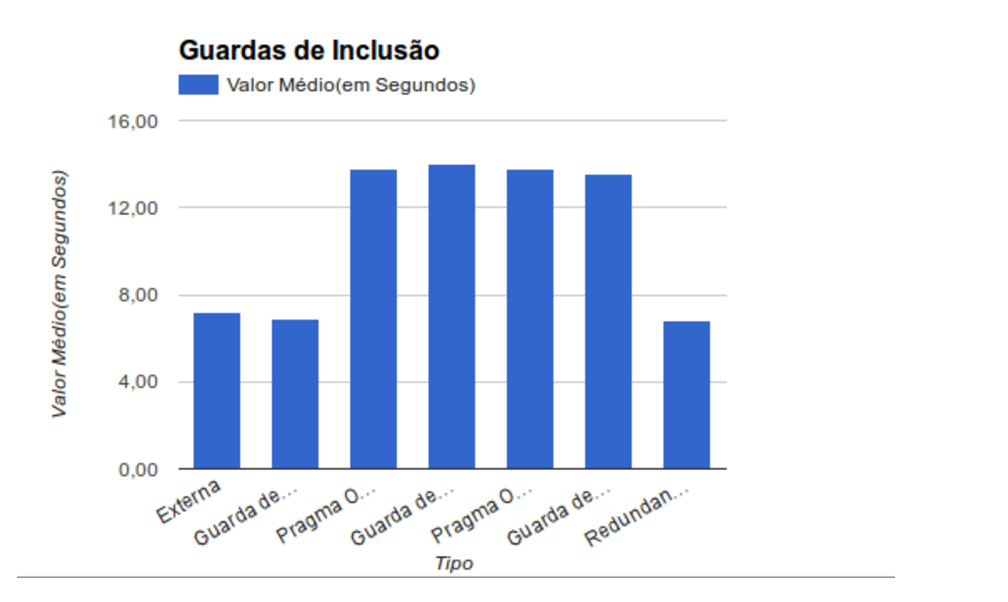
\includegraphics[keepaspectratio=true,scale=1]{figuras/guardas_de_inclusao.eps}
    \caption{Gráfico de redução em segundos para cada método guarda de inclusão}
    \label{grafico_guardas_de_inclusao}
\end{figure}


\section{Segundo Experimento}


A Tabela \ref{experimento_02} e o Gráfico \ref{grafico_forward_declaration} apresentam os resultados do
 segundo experimento, que avalia o uso das forward declarations.Fator de
 Redução é igual a 1 menos o tempo sem forward declaration divido pelo
 tempo com forward declaration.



\begin{table}[h]
\centering
\begin{tabular}{|l|p{3cm}|p{3cm}|p{3cm}|}
\hline
Tipo       & \multicolumn{3}{l|}{Forward Declaration}                                                                                                                            \\ \hline
Tempo      & \multicolumn{3}{l|}{Em segundos}                                                                                                                                    \\ \hline
Repetições & Tempo de Compilação SEM forward Declaration & Tempo de Compilação COM Forward Declaration & Fator de Redução) \\ \hline
1      & 5,11  & 5,042 & 1,3\% \\ \hline
2      & 5,07  & 4,984 & 1,8\% \\ \hline
3      & 5,12  & 5,055 & 1,3\% \\ \hline
4      & 5,12  & 4,937 & 3,5\% \\ \hline
5      & 5,18  & 5,153 & 0,5\% \\ \hline
6      & 5,20  & 5,045 & 3,1\% \\ \hline
7      & 5,15  & 4,986 & 3,1\% \\ \hline
8      & 5,21  & 5,151 & 1,0\% \\ \hline
9      & 5,21  & 5,045 & 3,1\% \\ \hline
10     & 5,13  & 5,09  & 0,8\% \\ \hline
Média  & 5,15  & 5,05  & 1,9\% \\ \hline
\end{tabular}
\caption{resultado das experimentos forward declaration}
\label{experimento_02}
\end{table}


\begin{figure}[h]
    \centering
        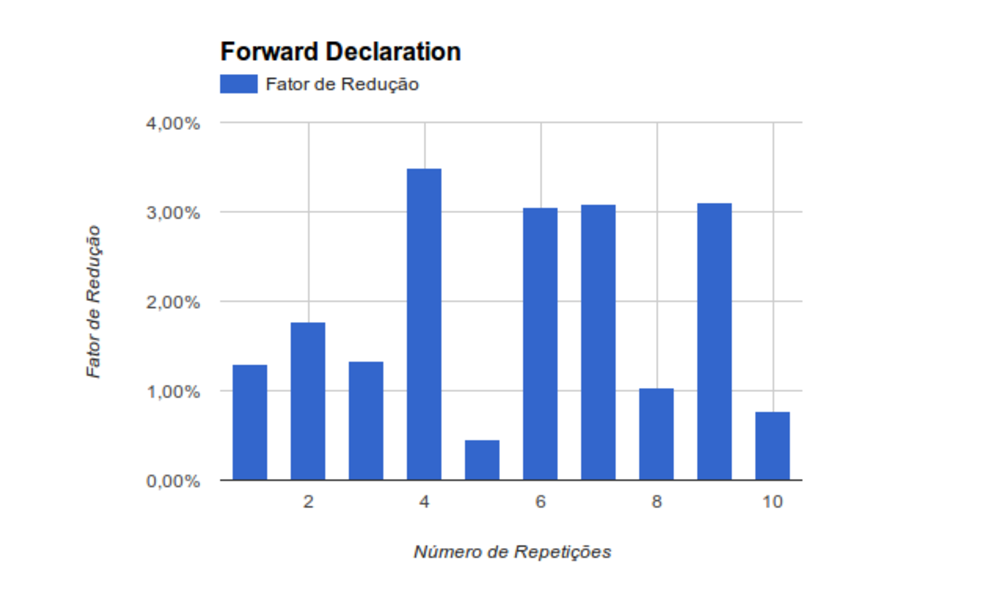
\includegraphics[keepaspectratio=true,scale=1]{figuras/forward_declaration.eps}
    \caption{Gráfico de fator de redução para cada dado coletado}
    \label{grafico_forward_declaration}
\end{figure}



A Tabela \ref{experimento_02} mostra os valores coletados durante
 os experimentos de forward declaration. O Gráfico
 \ref{grafico_forward_declaration} demonstra que todos os valores
 foram positivos, indicando que forward declaration reduziu o tempo
 de compilação em todos os casos, com uma variação de 0,5\% a 3,1\%.




\begin{table}[h]
\centering
\begin{tabular}{|p{3cm}|p{3cm}|p{3cm}|p{3cm}|}
\hline
Tempo      & \multicolumn{3}{l|}{Em segundos}    \\ \hline
Quantidade de Modificações & Sem forward Declaration  & Com forward Declaration & Fator de Redução\\ \hline
1  & 2,01 & 1,61 & 19,90\% \\ \hline
15 & 4,2  & 3,48 & 17,14\% \\ \hline
4  & 4,48 & 4,45 & 0,67\% \\ \hline
1  & 2,01 & 1,56 & 22,39\% \\ \hline
4  & 2,32 & 2,07 & 10,78\% \\ \hline
12 & 4,44 & 4,46 & -0,45\% \\ \hline
12 & 5,03 & 4,26 & 15,31\% \\ \hline
8  & 4,83 & 4,38 & 9,32\% \\ \hline
12 & 4,43 & 3,36 & 24,15\% \\ \hline
4  & 4,38 & 4,31 & 1,60\% \\ \hline
Média  & 3,81  & 3,39  & 10,99\% \\ \hline 
\end{tabular}
\caption{Realizando modificações parciais nos Códigos}
\label{amostas_experimento_03}
\end{table}


\begin{figure}[h]
    \centering
        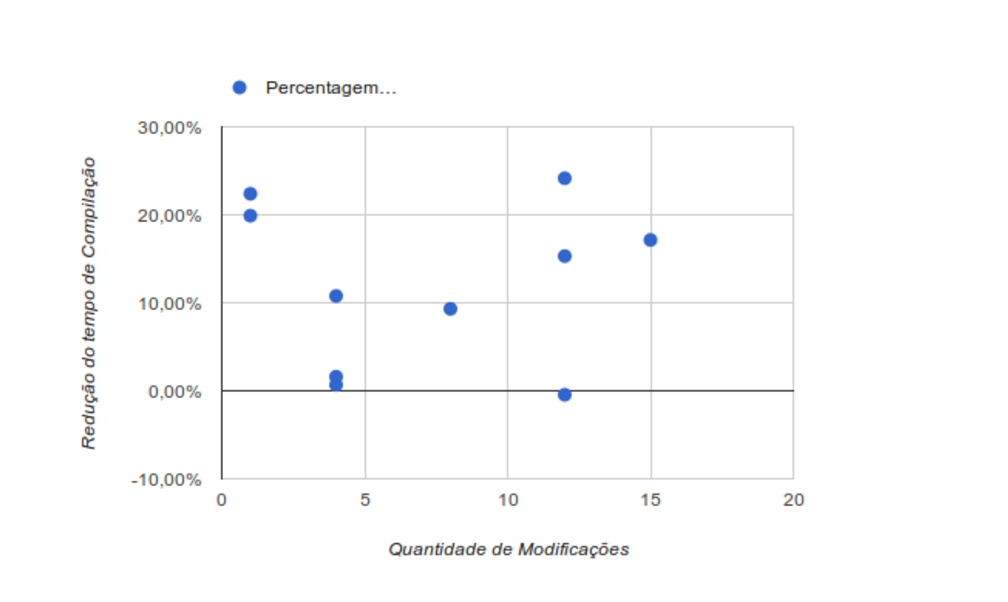
\includegraphics[keepaspectratio=true,scale=1]{figuras/forward_declaration2.eps}
    \caption{Dados utilizando script de modificações}
    \label{grafico_forward_declaration2}
\end{figure}

A figura \ref{grafico_forward_declaration2} representa a utilização
 do Código \ref{script_forward_declaration},
 que realiza modificações na data de modifição de um arquivo, o que forca uma
 recompilação do mesmo na próxima invocação do comando make.
 Esta tabela mostra que realizando modificações em diferentes
 quantidades de arquivos o beneficio do forward declaration é
 diretamente impactado. Ainda assim, apenas em uma amostra o percentual
 de redução foi negativo  (isto é, houve um acréscimo de tempo,
 em relação a média), no entanto com uma variação baixa.



\section{Terceiro Experimento}

O terceiro experimento avaliou o impacto da compilação
 paralela através do uso da flag \texttt{-j} do
 comando make (Seção \ref{experimento_03}).



\textbf{CPPCheck}:


\begin{table}[h]
\centering
\begin{tabular}{|p{1cm}|p{1.4cm}|p{1.4cm}|p{1.4cm}|p{1.4cm}|p{1.4cm}|p{1.4cm}|p{1.4cm}|p{1.4cm}|p{1.4cm}|}
\hline
Projeto               & \multicolumn{9}{l|}{CPPCheck}        \\ \hline
Tempo                 & \multicolumn{9}{l|}{Em segundos}      \\ \hline
Quantidade de Threads & 1 & 2 & 4 & 6 & 8 & 10 & 12 & 14 & 16 \\ \hline
Repetições            & - & - & - & - & - & -  & -  & -  & -  \\ \hline
1 & 156,55  &  117,06  &  99,49   &  89,60    & 100,10   & 110,24  & 95,44     & 104,99   & 136,11 \\ \hline
2 & 158,594 &  121,217 &  114,765 &  99,578   & 100,418  & 98,722  & 119,161   & 117,518  & 113,762 \\ \hline
3 & 148,788 &  122,364 &  117,067 &  112,585  & 98,579   & 95,049  & 114,737   & 102,282  & 101,268 \\ \hline
4 & 150,221 &  127,157 &  93,796  &  101,384  & 103,777  & 96,115  & 109,047   & 120,619  & 101,821 \\ \hline
5 & 151,573 &  134,801 &  99,205  &  91,467   & 99,23    & 91,805  & 110,559   & 116,869  & 101,707 \\ \hline
6 & 157,699 &  113,408 &  105,849 &  97,544   & 105,757  & 94,618  & 104,659   & 119,882  & 128,401 \\ \hline
7 & 160,904 &  117,252 &  100,824 &  106,545  & 101,3    & 120,292 & 102,033   & 110,102  & 101,852 \\ \hline
8 & 163,585 &  116,945 &  99,559  &  102,174  & 104,513  & 101,237 & 101,548   & 115,973  & 114,179 \\ \hline
9 & 162,394 &  118,116 &  95,91   &  100,858  & 108,575  & 98,31   & 113,773   & 93,53    & 113,304 \\ \hline
10& 163,483 &  110,68  &  109,524 &  105,307  & 100,16   & 111,89  & 94,516    & 94,674   & 119,209 \\ \hline
Média& 157,3787&  119,8999&  103,5988&  100,7035 & 102,2404 & 101,8278&  106,5477 & 109,6446 & 113,1615 \\ \hline
\end{tabular}
\caption{CppCheck utilizando jobs do makefile}
\label{tab:cppcheck}
\end{table}


\begin{figure}[h]
    \centering
        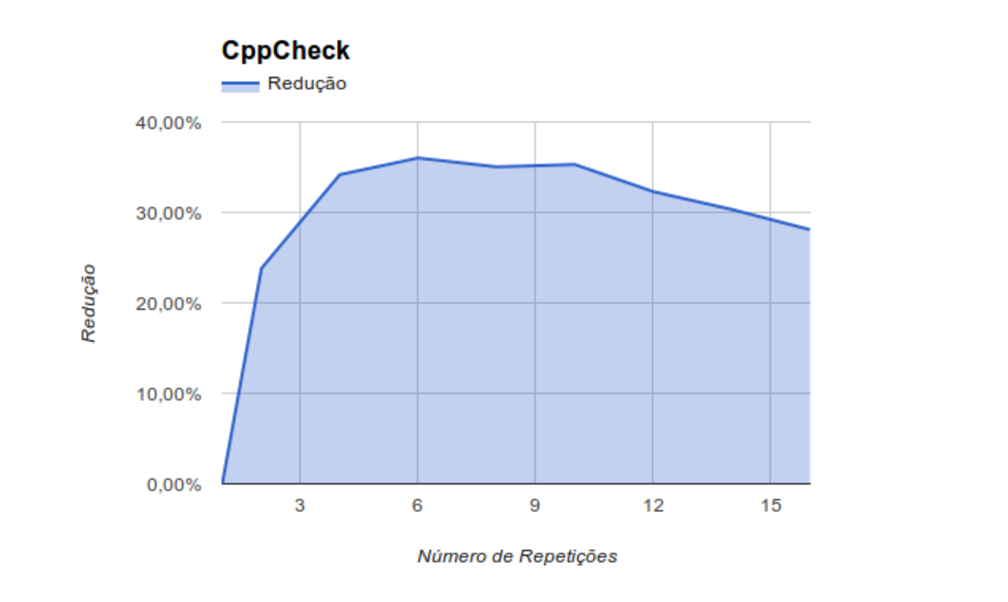
\includegraphics[keepaspectratio=true,scale=1]{figuras/cppcheck.eps}
    \caption{Gráfico de redução do tempo de compilação para projeto CppCheck}
    \label{cppcheck}
\end{figure}

Analisando os resultados dos experimentos realizados com o projeto
 CppCheck, apresentados na tabela \ref{tab:cppcheck} e no Gráfico \ref{cppcheck},
 que indica um gráfico das porcentagens de redução, é
 possivel afirmar que utilizar mais de uma thread para a
 compilação pode trazer uma redução no tempo de compilação.
 Neste projeto o beneficio da redução foi de 20\% a 35\%.
 É possível observar que o aumento das threads  não
 necessariamente aumenta a redução do tempo de compilação,
 uma vez que com 16 threads  a redução foi menor  do que com 12 threads.


\textbf{Hayai}


\begin{table}[h]
\centering
\begin{tiny}
\begin{tabular}{cccccccccc}
\toprule
\textbf{Repetições} & \multicolumn{9}{c}{\textbf{Número de threads}} \\ \midrule
- & 1 & 2 & 4 & 6 & 8 & 10 & 12 & 14 & 16 \\ 
1 & 3,443 & 2,964  & 2,523 &2,276 &2,624    & 2,612   &2,425    &2,389  &2,496  \\ 
2 & 3,287 & 2,43   & 2,374 &2,24  &2,53     & 2,66    &2,39     &2,748  &2,426   \\ 
3 & 3,622 & 2,531  & 2,489 &2,316 &2,673    & 2,737   &2,51     &2,46   &2,523 \\ 
4 & 3,456 & 2,906  & 2,468 &2,285 &2,534    & 2,399   &2,849    &2,707  &2,485 \\ 
5 & 3,816 & 2,498  & 2,466 &2,509 &2,568    & 2,416   &2,499    &2,718  &2,683 \\ 
6 & 3,757 & 2,415  & 2,457 &2,283 &2,735    & 2,539   &2,588    &2,584  &2,548 \\ 
7 & 3,504 & 2,604  & 2,549 &2,578 &2,621    & 2,621   &2,532    &2,398  &2,676 \\ 
8 & 3,404 & 2,451  & 2,433 &2,274 &2,533    & 2,683   &2,542    &2,502  &2,895 \\ 
9 & 3,564 & 2,474  & 2,886 &2,197 &2,902    & 2,399   &2,475    &2,82   &2,476 \\ 
10 & 3,482 & 2,571  & 2,458 &2,618 &2,618    & 2,623   &2,381    &2,755  &2,816 \\ \midrule
Média & 3,5335 &  2,5844 & 2,5103 & 2,357 & 2,6338 & 2,5689 & 2,5191 &2,6081 &2,6024 \\ \bottomrule
\end{tabular}
\end{tiny}
\caption{Hayai utilizando jobs do makefile}
\label{tab:hayai}
\end{table}

\begin{figure}[h]
    \centering
        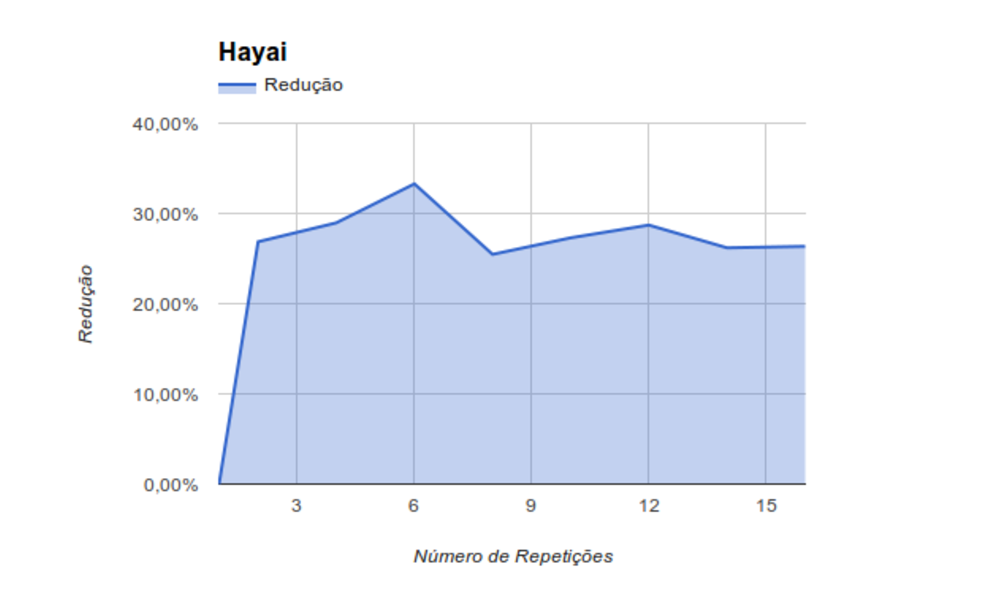
\includegraphics[keepaspectratio=true,scale=1]{figuras/hayai.eps}
    \caption{Gráfico de redução do tempo de compilação para projeto CppCheck}
    \label{hayai}
\end{figure}

Analisando os experimentos realizados com o hayai foi evidenciado ganho
 na redução do tempo de compilação do projeto, e com os mesmos
 observações do cppcheck. Neste caso com 16 threads foi maior que com
 12 threads. Neste projeto o ganho da redução do tempo de
 compilação varia entre 20\% e 32\%.

\textbf{JsonCpp}


\begin{table}[h]
\centering
\begin{tabular}{|p{1cm}|p{1.4cm}|p{1.4cm}|p{1.4cm}|p{1.4cm}|p{1.4cm}|p{1.4cm}|p{1.4cm}|p{1.4cm}|p{1.4cm}|}
\hline
Projeto               & \multicolumn{9}{l|}{JsonCpp}        \\ \hline
Tempo                 & \multicolumn{9}{l|}{Em segundos}      \\ \hline
Quantidade de Threads & 1 & 2 & 4 & 6 & 8 & 10 & 12 & 14 & 16 \\ \hline
Repetições            & - & - & - & - & - & -  & -  & -  & -  \\ \hline
1 & 16,013   & 11,599  & 11,117  & 9,838   & 12,202  & 10,114  & 11,366  & 10,966  & 12,108 \\ \hline
2 & 15,12    & 12,632  & 11,429  & 12,635  & 10,023  & 10,06   & 11,189  & 9,987   & 11,054 \\ \hline
3 & 14,932   & 11,967  & 10,48   & 10,098  & 11,136  & 11,24   & 9,862   & 10,177  & 10,285 \\ \hline
4 & 15,066   & 11,86   & 10,198  & 10,282  & 11,771  & 12,492  & 12,318  & 10,22   & 9,793 \\ \hline
5 & 15,202   & 11,383  & 10,112  & 10,882  & 10,714  & 10,476  & 9,991   & 10,917  & 10,033 \\ \hline
6 & 15,013   & 11,458  & 11,299  & 9,998   & 10,35   & 9,944   & 11,223  & 10,053  & 11,158 \\ \hline
7 & 14,98    & 11,519  & 10,909  & 9,95    & 11,481  & 11,105  & 11,071  & 11,19   & 11,288 \\ \hline
8 & 15,074   & 12,387  & 10,936  & 11,925  & 9,971   & 11,198  & 10,843  & 10,161  & 11,679 \\ \hline
9 & 15,361   & 11,668  & 11,74   & 11,229  & 12,218  & 10,222  & 10,551  & 10,019  & 9,879 \\ \hline
10 & 15,124   & 11,435  & 10,583  & 11,031  & 11,167  & 10,12   & 12,721  & 12,412  & 10,131 \\ \hline
Média & 15,1885  & 11,7908 & 10,8803 & 10,7868 & 11,1033 & 10,6971 & 11,1135 & 10,6102 & 10,7408 \\ \hline
\end{tabular}
\caption{jsoncpp utilizando jobs do makefile}
\label{tab:jsoncpp}
\end{table}


\begin{figure}[h]
    \centering
        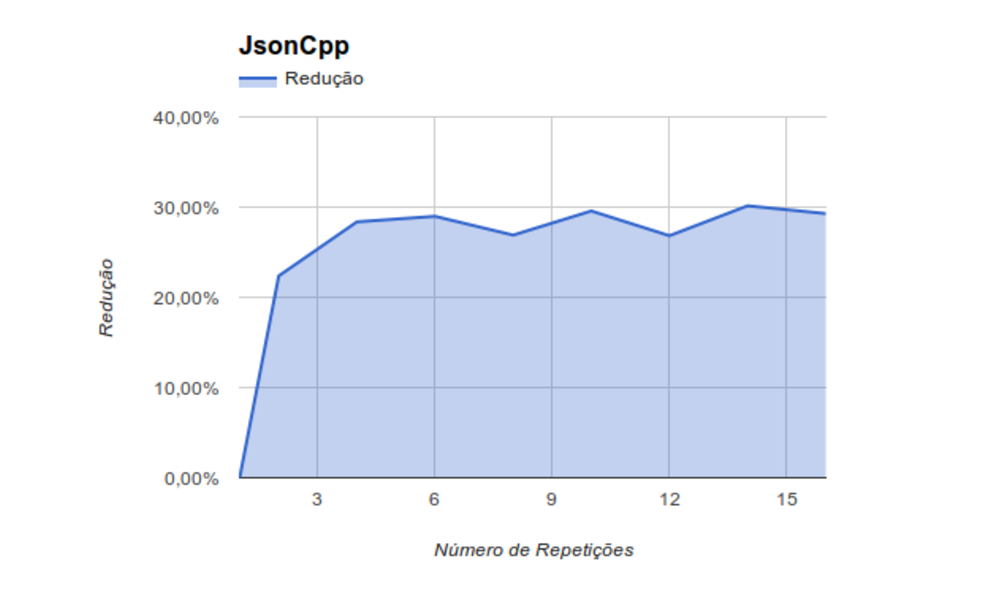
\includegraphics[keepaspectratio=true,scale=1]{figuras/jsoncpp.eps}
    \caption{Gráfico de redução do tempo de compilação para projeto JsonCpp}
    \label{jsoncpp}
\end{figure}

Analisando os dados coletados no projeto Jsoncpp, é observado
 que o uso de thread proporciona
 redução do tempo de compilação, variando de 20\% a 31\%.
As mesmas observações encontradas no CppCheck.

\textbf{LibSass}

\begin{table}[h]
\centering
\begin{tabular}{|p{1cm}|p{1.4cm}|p{1.4cm}|p{1.4cm}|p{1.4cm}|p{1.4cm}|p{1.4cm}|p{1.4cm}|p{1.4cm}|p{1.4cm}|}
\hline
Projeto               & \multicolumn{9}{l|}{LibSass}        \\ \hline
Tempo                 & \multicolumn{9}{l|}{Em segundos}      \\ \hline
Quantidade de Threads & 1 & 2 & 4 & 6 & 8 & 10 & 12 & 14 & 16 \\ \hline
Repetições            & - & - & - & - & - & -  & -  & -  & -  \\ \hline
1 & 52,448   & 42,562   & 32,535   & 42,828   & 31,111  & 31,391  & 31,625  & 31,508  & 31,965 \\ \hline
2 & 51,94    & 38,296   & 41,006   & 34,674   & 38,298  & 42,883  & 31,326  & 37,236  & 31,646 \\ \hline
3 & 51,632   & 39,621   & 43,227   & 33,82    & 31,341  & 47,873  & 32,94   & 32,237  & 39 \\ \hline
4 & 51,844   & 44,601   & 43,514   & 34,241   & 31,272  & 42,377  & 31,196  & 38,772  & 46,834 \\ \hline
5 & 51,165   & 38,335   & 33,511   & 43,01    & 38,582  & 47,222  & 31,56   & 46,99   & 34,354 \\ \hline
6 & 52,032   & 37,376   & 30,897   & 34,612   & 34,98   & 36,43   & 32,435  & 31,407  & 31,713 \\ \hline
7 & 51,525   & 36,105   & 42,818   & 30,831   & 36,641  & 37,691  & 40,757  & 38,838  & 31,59 \\ \hline
8 & 51,907   & 33,804   & 35,54    & 32,129   & 31,511  & 31,77   & 32,175  & 32,414  & 40,088 \\ \hline
9 & 51,79    & 43,258   & 31,919   & 30,811   & 34,529  & 47,326  & 32,586  & 39,355  & 38,228 \\ \hline
10& 52,046   & 40,352   & 46,493   & 37,484   & 42,191  & 41,195  & 31,749  & 37,03   & 31,607 \\ \hline
Média& 51,8329  & 39,431   & 38,146   & 35,444   & 35,0456 & 40,6158 & 32,8349 & 36,5787 & 35,7025 \\ \hline
\end{tabular}
\caption{LibSass utilizando jobs do makefile}
\label{tab:libsass}
\end{table}


\begin{figure}[h]
    \centering
        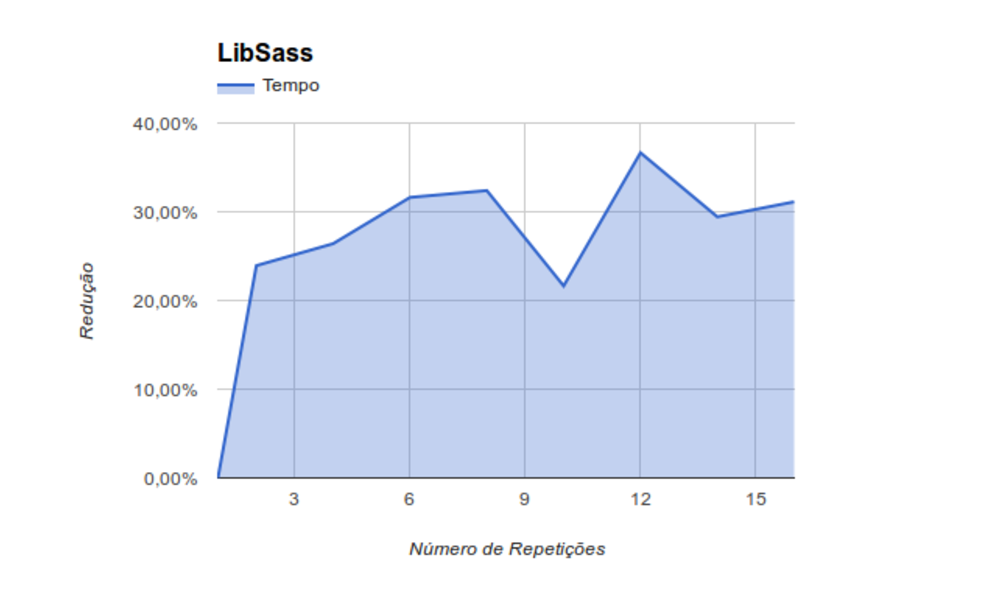
\includegraphics[keepaspectratio=true,scale=1]{figuras/libsass.eps}
    \caption{gráfico de redução do tempo de compilação para projeto libsass}
    \label{libsass}
\end{figure}

Analisado as amostras para o projeto Libsass, é confirmado que o
 uso de threads reduziu o tempo de compilação e com variação
 de 20\% a 35\% de redução do tempo de compilação.

\textbf{LibOAuthCpp}

\begin{table}[h]
\centering
\begin{tabular}{|p{1cm}|p{1.4cm}|p{1.4cm}|p{1.4cm}|p{1.4cm}|p{1.4cm}|p{1.4cm}|p{1.4cm}|p{1.4cm}|p{1.4cm}|}
\hline
Projeto               & \multicolumn{9}{l|}{LibOAuthCpp}        \\ \hline
Tempo                 & \multicolumn{9}{l|}{Em segundos}      \\ \hline
Quantidade de Threads & 1 & 2 & 4 & 6 & 8 & 10 & 12 & 14 & 16 \\ \hline
Repetições            & - & - & - & - & - & -  & -  & -  & -  \\ \hline
1 & 13,057   & 12,295   & 12,289   & 12,217   &  11,632   &  11,743  &  12,406  &   12,116  &   11,798 \\ \hline
2 & 13,213   & 12,218   & 12,368   & 11,682   &  12,181   &  11,792  &  11,716  &   12,224  &   11,681 \\ \hline
3 & 13,302   & 11,689   & 12,149   & 12,007   &  12,038   &  11,724  &  11,993  &   12,458  &   11,821 \\ \hline
4 & 13,054   & 12,219   & 11,987   & 12,071   &  11,614   &  11,722  &  11,702  &   11,662  &   12,069 \\ \hline
5 & 13,113   & 12,261   & 12,073   & 11,671   &  12,345   &  11,988  &  11,662  &   11,935  &   11,651 \\ \hline
6 & 13,392   & 12,109   & 11,908   & 11,753   &  12,402   &  11,812  &  12,366  &   11,732  &   12,066 \\ \hline
7 & 13,125   & 12,012   & 12,075   & 11,809   &  11,614   &  11,707  &  12,304  &   12,333  &   11,679 \\ \hline
8 & 13,241   & 11,981   & 11,725   & 11,762   &  11,847   &  12,426  &  12,043  &   12,588  &   11,993 \\ \hline
9 & 13,021   & 12,09    & 11,864   & 11,708   &  11,904   &  12,014  &  12,709  &   12,151  &   12,007 \\ \hline
10 & 13,644   & 12,348   & 12,267   & 12,288   &  12,251   &  11,884  &  12,56   &   11,892  &   12,557 \\ \hline
Média & 13,2162  & 12,1222  & 12,0705  & 11,8968  &  11,9828  &  11,8812 &  12,1461 &   12,1091 &   11,9322 \\ \hline
\end{tabular}
\caption{LibOAuthCpp utilizando jobs do makefile}
\label{tab:liboauthcpp}
\end{table}


\begin{figure}[h]
    \centering
        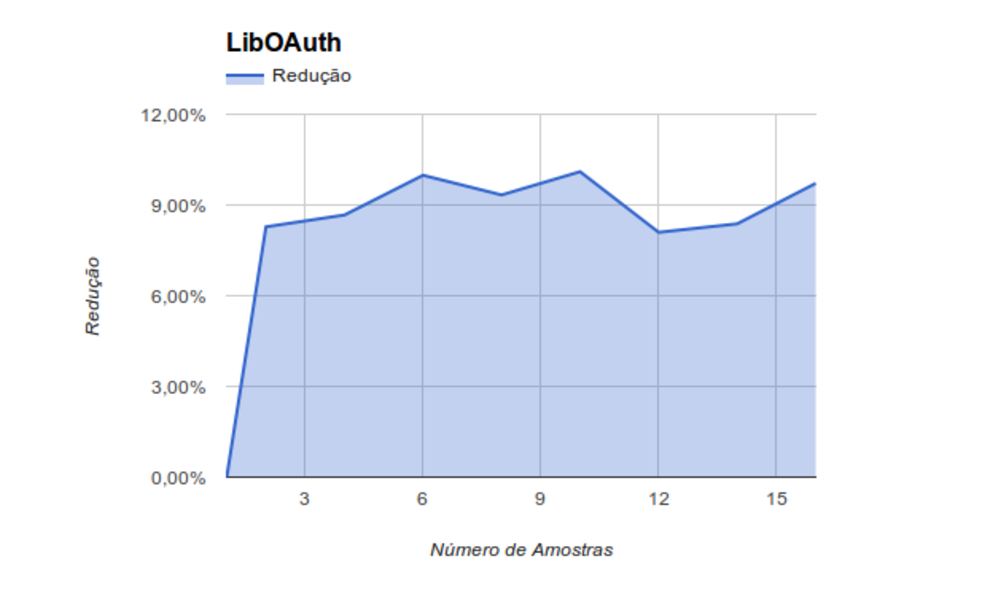
\includegraphics[keepaspectratio=true,scale=1]{figuras/liboauth.eps}
    \caption{gráfico de redução do tempo de compilação para projeto LibOAuth}
    \label{liboauth}
\end{figure}

Analisando a coleta de dados do projeto LibSass, é evidenciado que ele possui
 redução do tempo de compilação , no entanto este projeto não teve ganhos
 acima de 10\%. Este valores são totalmente diferentes dos outros projetos,
 então a estrutura do projeto pode ter influenciado na redução do
 tempo de compilação. 

\textbf{Jack, the Janitor}

\begin{table}[h]
\centering
\begin{tabular}{|p{1cm}|p{1.4cm}|p{1.4cm}|p{1.4cm}|p{1.4cm}|p{1.4cm}|p{1.4cm}|p{1.4cm}|p{1.4cm}|p{1.4cm}|}
\hline
Projeto               & \multicolumn{9}{l|}{Jack, The Janitor} \\ \hline
Tempo                 & \multicolumn{9}{l|}{Em segundos}      \\ \hline
Quantidade de Threads & 1 & 2 & 4 & 6 & 8 & 10 & 12 & 14 & 16 \\ \hline
Repetições            & - & - & - & - & - & -  & -  & -  & -  \\ \hline
1 & 5,21    & 2,24  &  2,13   & 2,15   & 2,19   & 2,32   & 2,41  &  2,73  & 2,25 \\ \hline
2 & 3,92    & 2,44  &  2,73   & 2,21   & 2,24   & 2,23   & 2,38  &  2,33  & 2,29 \\ \hline
3 & 3,94    & 2,51  &  2,84   & 2,28   & 2,24   & 2,27   & 2,22  &  2,34  & 3,01 \\ \hline
4 & 4,02    & 2,64  &  2,46   & 2,22   & 2,22   & 2,19   & 2,28  &  2,23  & 2,26 \\ \hline
5 & 3,87    & 2,51  &  2,32   & 2,29   & 2,64   & 2,51   & 2,25  &  2,33  & 2,74 \\ \hline
6 & 3,81    & 2,91  &  2,30   & 2,27   & 2,63   & 2,30   & 2,26  &  2,23  & 3,14 \\ \hline
7 & 3,91    & 2,40  &  2,28   & 2,17   & 2,40   & 3,09   & 2,74  &  2,33  & 2,35 \\ \hline
8 & 3,88    & 2,39  &  2,52   & 2,34   & 2,34   & 2,31   & 2,27  &  2,31  & 3,00 \\ \hline
9 & 3,93    & 2,54  &  2,87   & 2,38   & 2,31   & 2,26   & 3,02  &  2,37  & 2,40 \\ \hline
10 & 3,84    & 3,10  &  2,85   & 2,23   & 2,22   & 2,18   & 2,75  &  2,35  & 3,04 \\ \hline
Média & 4,0308  & 2,5651&  2,5293 & 2,2547 & 2,3426 & 2,3657 & 2,4565&  2,3529 & 2,6473 \\ \hline
\end{tabular}
\caption{Jack, the Janitor utilizando jobs do makefile}
\label{tab:janitor}
\end{table}


\begin{figure}[h]
    \centering
        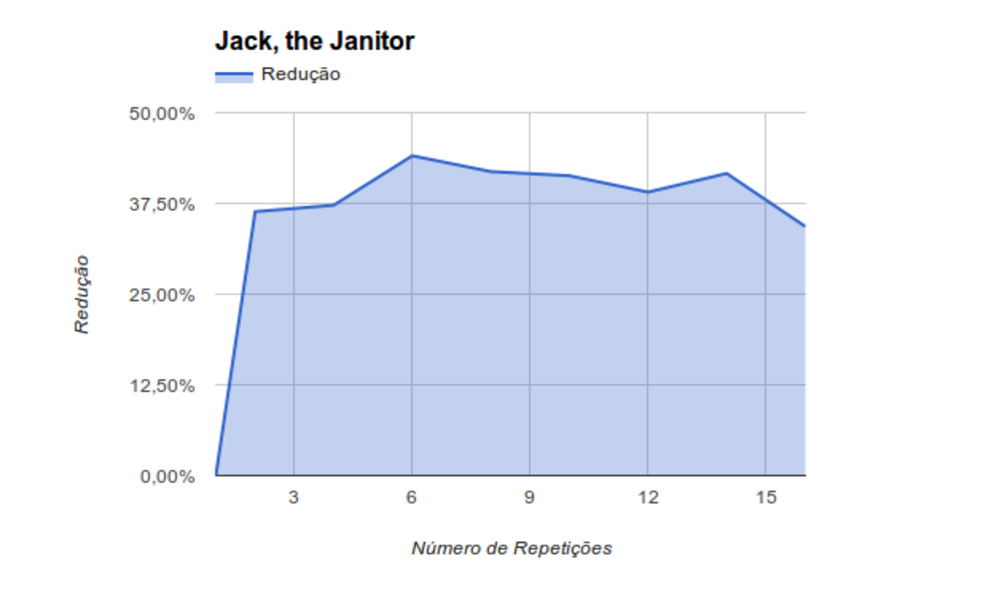
\includegraphics[keepaspectratio=true,scale=1]{figuras/jack.eps}
    \caption{gráfico de redução do tempo de compilação para projeto Jack, the Janitor}
    \label{jack}
\end{figure}

Analisando os dados coletados do projeto Jack,the Janitor,
 percebemos as mesmas reduções entre os projetos anteriores
 e ainda mais neste projeto as os ganhos da redução do
 tempo de compilação foram maiores.

Após a coleta dos dados dos 6 projetos distintos podemos
 perceber que não há uma relação direta entre as diferentes
 quantidades de threads. Isto é observado nos gráficos,
 com o aumento das threads não necessariamente implicando
 em um aumento proporcional. Os dados encontrados
 sugerem que este método pode reduzir o tempo de
 compilação em aproximadamente 20\%.

\part{Conclusão}

\chapter[Considerações Finais]{Considerações Finais}

\section{Conclusões}

\section{Trabalhos Futuros}



\bookmarksetup{startatroot} 

\postextual

\bibliography{bibliografia} 
\begin{apendicesenv}

\partapendices

\chapter{Script Aplicado ao Ambiente}

\section{Gerador de Codigo para Benchmark}

\subsection{Guardas de Inclusão Externa mais Pragma Once}
\begin{lstlisting}[language=Python, caption={
     Script Guardas de Inclusão Externa mais pragma once},
                  label=script_external_pragma_include]

# external_pragma.py
from os import mkdir
from os import path
from os import system

number_of_files = 10**4
number_of_includes = 3

folder =  "./external_pragma/"

include_directory = folder+"include"
include_path = folder+"include/{0}.hpp"
path_main_file = folder+"main.cpp"

content_of_include = """#pragma once\nconst int int{0} = {0};"""
end_of_main_file = "int main() {\n}\n"
header = """#ifndef H{0}_HPP
#define H{0}_HPP
#include "{0}.hpp"
#endif
"""

def verify_directory(path_name):
    if not path.exists(path_name):
        mkdir(path_name)

def create_include_file(path,content):
    f =  open(path,"w+")
    f.write (content)
    f.close()

def create_includes():
    #create directory
    # create all files
    for number in range(0,number_of_files):
        path = include_path.format(str(number))
        content = content_of_include.format(str(number))
        create_include_file(path,content)
    
def create_main_file():
    #open main.cpp
    main = open(path_main_file,"w+")

    #write includes 3 times
    for number in range(0,number_of_files):
        for x in range(0,number_of_includes):
            content = header.format(str(number))
            main.write(content)
        main.write("\n")

    #write end of file
    main.write(end_of_main_file)

    #close main.cpp
    main.close()
                                                                                  
def copy_util_files():                                                           
    command = "cp util/* "                                                       
    command += folder                                                            
    system(command)      

def main():
    verify_directory(folder)
    verify_directory(include_directory)
    create_includes()
    create_main_file()
    copy_util_files()

if __name__ == "__main__":
    main()
\end{lstlisting}

\subsection{Guardas de Inclusão Externa}
\begin{lstlisting}[language=Python,caption={
            Script Guardas de Inclusão Externa },
                   label=script_external_include]
                   
                   
# external.py
from os import mkdir
from os import path
from os import system

number_of_files = 10**4
number_of_includes = 3

folder =  "./external/"

include_directory = folder+"include"
include_path = folder+"include/{0}.hpp"
path_main_file = folder+"main.cpp"

content_of_include = """const int int{0} = {0};"""
end_of_main_file = "int main() {\n}\n"
header = """#ifndef H{0}_HPP
#define H{0}_HPP
#include "{0}.hpp"
#endif
"""

def verify_directory(path_name):
    if not path.exists(path_name):
        mkdir(path_name)

def create_include_file(path,content):
    f =  open(path,"w+")
    f.write (content)
    f.close()

def create_includes():
    #create directory
    # create all files
    for number in range(0,number_of_files):
        path = include_path.format(str(number))
        content = content_of_include.format(str(number))
        create_include_file(path,content)
    
def create_main_file():
    #open main.cpp
    main = open(path_main_file,"w+")

    #write includes 3 times
    for number in range(0,number_of_files):
        for x in range(0,number_of_includes):
            content = header.format(str(number))
            main.write(content)
        main.write("\n")

    #write end of file
    main.write(end_of_main_file)

    #close main.cpp
    main.close()

def copy_util_files():
    command = "cp util/* "
    command += folder
    system(command)
    

def main():
    verify_directory(folder)
    verify_directory(include_directory)
    create_includes()
    create_main_file()
    copy_util_files()

if __name__ == "__main__":
    main()
\end{lstlisting}

\subsection{Guardas de Inclusão Interna}
\begin{lstlisting}[language=Python,caption={
              Script Guardas de Inclusão Interna},
                     label=script_intenal_include]
                     
# guard_only.py
from os import mkdir
from os import path
from os import system

number_of_files = 10**4
number_of_includes = 3

folder =  "./guard-only/"

include_directory = folder+"include"
include_path = folder+"include/{0}.hpp"
path_main_file = folder+"main.cpp"

content_of_include = """#ifndef H{0}_HPP
#define H{0}_HPP
const int int{0} = {0};
#endif
"""

end_of_main_file = "int main() {\n}\n"
header = "#include \"{0}.h\"\n"

def verify_directory(path_name):
    if not path.exists(path_name):
        mkdir(path_name)

def create_include_file(path,content):
    f =  open(path,"w+")
    f.write (content)
    f.close()

def create_includes():
    #create directory
    # create all files
    for number in range(0,number_of_files):
        path = include_path.format(str(number))
        content = content_of_include.format(str(number))
        create_include_file(path,content)
    
def create_main_file():
    #open main.cpp
    main = open(path_main_file,"w+")

    #write includes 3 times
    for number in range(0,number_of_files):
        for x in range(0,number_of_includes):
            content = header.format(str(number))
            main.write(content)
        main.write("\n")

    #write end of file
    main.write(end_of_main_file)

    #close main.cpp
    main.close()
                                                                                  
def copy_util_files():                                                           
    command = "cp util/* "                                                       
    command += folder                                                            
    system(command)      

def main():
    verify_directory(folder)
    verify_directory(include_directory)
    create_includes()
    create_main_file()
    copy_util_files()

if __name__ == "__main__":
    main()
\end{lstlisting}

\subsection{Guardas de Inclusão Interna primeiro que o Pragma Once}
\begin{lstlisting}[language=Python, caption={
Script Guardas de Inclusão Interna primeiro que \textit{Pragma Once}},
                   label=script_guards_pragma_include]
                   
# guards_pragma.py
from os import mkdir
from os import path
from os import system

number_of_files = 10**4
number_of_includes = 3

folder =  "./guards-pragma/"

include_directory = folder+"include"
include_path = folder+"include/{0}.hpp"
path_main_file = folder+"main.cpp"

content_of_include = """#ifndef H{0}_HPP
#define H{0}_HPP
#pragma once
const int int{0} = {0};
#endif
"""

end_of_main_file = "int main() {\n}"
header = """#include "{0}.hpp"\n"""

def verify_directory(path_name):
    if not path.exists(path_name):
        mkdir(path_name)

def create_include_file(path,content):
    f =  open(path,"w+")
    f.write (content)
    f.close()

def create_includes():
    #create directory
    # create all files
    for number in range(0,number_of_files):
        path = include_path.format(str(number))
        content = content_of_include.format(str(number))
        create_include_file(path,content)
    
def create_main_file():
    #open main.cpp
    main = open(path_main_file,"w+")

    #write includes 3 times
    for number in range(0,number_of_files):
        for x in range(0,number_of_includes):
            content = header.format(str(number))
            main.write(content)

    #write end of file
    main.write(end_of_main_file)

    #close main.cpp
    main.close()
def copy_util_files():                                                           
    command = "cp util/* "                                                       
    command += folder                                                            
    system(command)                                                              
                    

def main():
    verify_directory(folder)
    verify_directory(include_directory)
    create_includes()
    create_main_file()
    copy_util_files()

if __name__ == "__main__":
    main()
\end{lstlisting}

\subsection{Guardas de Inclusão com Pragma Once primeiro que Inclusão Interna}
\begin{lstlisting}[language=Python, caption={
    Script \textit{Pragma Once} primeiro que Guardas de Inclusão Interna},label=script_pragma_guards_include]
    
# pragma_guards.py
from os import mkdir
from os import path
from os import system

number_of_files = 10**4
number_of_includes = 3

folder =  "./pragma-guards/"

include_directory = folder+"include"
include_path = folder+"include/{0}.hpp"
path_main_file = folder+"main.cpp"

content_of_include = """#pragma once
#ifndef H{0}_HPP
#define H{0}_HPP
const int int{0} = {0};
#endif
"""

end_of_main_file = "int main() {\n}"
header = """#include "{0}.h"\n"""

def verify_directory(path_name):
    if not path.exists(path_name):
        mkdir(path_name)

def create_include_file(path,content):
    f =  open(path,"w+")
    f.write (content)
    f.close()

def create_includes():
    #create directory
    # create all files
    for number in range(0,number_of_files):
        path = include_path.format(str(number))
        content = content_of_include.format(str(number))
        create_include_file(path,content)
    
def create_main_file():
    #open main.cpp
    main = open(path_main_file,"w+")

    #write includes 3 times
    for number in range(0,number_of_files):
        for x in range(0,number_of_includes):
            content = header.format(str(number))
            main.write(content)

    #write end of file
    main.write(end_of_main_file)

    #close main.cpp
    main.close()
def copy_util_files():                                                           
    command = "cp util/* "                                                       
    command += folder                                                            
    system(command)                                                              

def main():
    verify_directory(folder)
    verify_directory(include_directory)
    create_includes()
    create_main_file()
    copy_util_files()

if __name__ == "__main__":
    main()
\end{lstlisting}

\subsection{Guardas Inclusão com Pragma Once}
\begin{lstlisting}[language=Python, caption={
                     Script Pragma Once},
             label=script_pragma_once_include]
             
# pragma_only.py
from os import mkdir
from os import path
from os import system

number_of_files = 10**4
number_of_includes = 3

folder =  "./pragma-only/"

include_directory = folder+"include"
include_path = folder+"include/{0}.hpp"
path_main_file = folder+"main.cpp"

content_of_include = """#pragma once
const int int{0} = {0};
"""

end_of_main_file = "int main() {\n}"
header = """#include "{0}.h"\n"""

def verify_directory(path_name):
    if not path.exists(path_name):
        mkdir(path_name)

def create_include_file(path,content):
    f =  open(path,"w+")
    f.write (content)
    f.close()

def create_includes():
    #create directory
    # create all files
    for number in range(0,number_of_files):
        path = include_path.format(str(number))
        content = content_of_include.format(str(number))
        create_include_file(path,content)
    
def create_main_file():
    #open main.cpp
    main = open(path_main_file,"w+")

    #write includes 3 times
    for number in range(0,number_of_files):
        for x in range(0,number_of_includes):
            content = header.format(str(number))
            main.write(content)

    #write end of file
    main.write(end_of_main_file)

    #close main.cpp
    main.close()
def copy_util_files():                                                           
    command = "cp util/* "                                                       
    command += folder                                                            
    system(command)                                                              
                      

def main():
    verify_directory(folder)
    verify_directory(include_directory)
    create_includes()
    create_main_file()
    copy_util_files()

if __name__ == "__main__":
    main()
\end{lstlisting}

\subsection{Guardas de Inclusão com Redundância}
\begin{lstlisting}[language=Python,caption={
     Script Redundância de Guardas de Inclusão},
                 label=script_redundante_include]
                 
# redundante.py
from os import mkdir
from os import path
from os import system

number_of_files = 10**4
number_of_includes = 3

folder =  "./redundant/"

include_directory = folder+"include"
include_path = folder+"include/{0}.hpp"
path_main_file = folder+"main.cpp"

content_of_include = """#ifndef H{0}_HPP
#define H{0}_HPP
const int int{0} = {0};
#endif"""
end_of_main_file = "int main() {\n}\n"
header = """#ifndef H{0}_HPP
#define H{0}_HPP
#include "{0}.hpp"
#endif
"""

def verify_directory(path_name):
    if not path.exists(path_name):
        mkdir(path_name)

def create_include_file(path,content):
    f =  open(path,"w+")
    f.write (content)
    f.close()

def create_includes():
    #create directory
    # create all files
    for number in range(0,number_of_files):
        path = include_path.format(str(number))
        content = content_of_include.format(str(number))
        create_include_file(path,content)
    
def create_main_file():
    #open main.cpp
    main = open(path_main_file,"w+")

    #write includes 3 times
    for number in range(0,number_of_files):
        for x in range(0,number_of_includes):
            content = header.format(str(number))
            main.write(content)
        main.write("\n")

    #write end of file
    main.write(end_of_main_file)

    #close main.cpp
    main.close()
def copy_util_files():                                                           
    command = "cp util/* "                                                       
    command += folder                                                            
    system(command)                                                              
                    

def main():
    verify_directory(folder)
    verify_directory(include_directory)
    create_includes()
    create_main_file()
    copy_util_files()

if __name__ == "__main__":
    main()

\end{lstlisting}


\chapter{Script Aplicado a Projeto}
\section{Recompilação de Projetos}
\begin{lstlisting}[language=Python, caption={Script de Recompilações},
                  label=script_recompilacoes]

        # *-* encoding: utf8 *-*
        from datetime import datetime
        from os import getcwd, chdir, makedirs, system
        from os.path import exists
        from yaml import load

        # common variables
        MAX_TIMES = 10
        current_dir = getcwd()
        output = current_dir+"/output/"
        config_file = current_dir+"/projects.yaml"

        def make_directories():
            if(not exists(output)):
                makedirs(output)

        def write_result(message, file_name):
            message += "\n"
            make_directories()
            _file = open(output+file_name, "a+")
            _file.write(message)
            _file.close()


        def change_to(directory):
            path = current_dir+"/"+directory
            chdir(path)
            print("Changed to {}".format(directory))


        def compile_project(command, project_debug):
            if not project_debug:
                command += " > /dev/null 2> /dev/null"

            system(command)


        def clean_projects(command, project_debug):
            if not project_debug:
                command += " > /dev/null 2> /dev/null"

            system(command)


        def wait_time():
            command = "sleep 1"
            system(command)


        def all_project(file_name):
            with open(file_name, 'r') as stream:
                content = load(stream)
            return content


        def set_branch(branch_name):
            command = "git checkout {}".format(branch_name)
            system(command)

        def exec_command(command):
            print "Using command %s"%(command)
            system(command)


        projects = all_project(config_file)

        if not projects:
            print("Need create a projects.yaml with projects attributes")

        else:
            for project_name, project in projects.items():
                print("Compiling [ {} ]".format(project_name))

                change_to(project['directory']+"/"+project['makefile'])

                for branch in project['branchs'] :
                    set_branch(branch['name'])

                    if branch['pre-command']:
                        for command in branch['pre-command']:
                            exec_command(command['command'])

                    message = "Branch [{}][{}]:".format(branch['name'],branch['description'])

                    write_result(message,project_name)

                    for times in range(0, MAX_TIMES):

                        clean_projects(branch['clean'], project['debug'])
                        wait_time()

                        start_time = datetime.now()
                        compile_project(branch['compile'], project['debug'])
                        end_time = datetime.now()

                        elapsed = end_time - start_time

                        text = "[{}/{}] : {:>4} ms".format(times+1, MAX_TIMES,
                                                              elapsed.total_seconds())

                        if not project['debug']:
                            print(text)

                        write_result(text, project_name)

                    write_result("*"*40+"", project_name)

                    if branch['pos-command']:
                        for command in branch['pos-command']:
                            exec_command(command['command'])

            print("Finished the result was saved in output folder")
\end{lstlisting}

\subsection{Template yaml para compilação de projetos}
\begin{lstlisting}[language=ruby, caption={Template para execução do Script de Recompilações},
                  label=template_para_script_recompilacoes]
    <project name>:
    directory:          <directory to project>
    makefile:           <path to make file into directory>
    debug:              <flag to see the project compilling>
    branchs:
       - name:          <branch to compile>
         description:   <little description>
         compile:        <line to compile the project>
         clean:            <line to clean the object compiled>
         pre-command:
              - command: <command executed before compile>
              - command: <command executed before compile>
              - command: <command executed before compile>
         pos-command:
              - command: <command executed after compile>
              - command: <command executed after compile>
              - command: <command executed after compile>
\end{lstlisting}

\end{apendicesenv}

\printindex

\end{document}

